\documentclass{report}
\RequirePackage[UTF8,scheme=plain]{ctex}
%\usepackage{xeCJK}
\usepackage{inputenc}

\usepackage[T1]{fontenc}
\usepackage{ccfonts, eulervm}

\usepackage{amsmath}
%\usepackage{amsthm}
\usepackage{ntheorem}
\usepackage{amssymb}
%\usepackage{amsfonts}
\usepackage{mathtools}
\usepackage{bm}
\usepackage{graphicx}
\usepackage[version=4]{mhchem}
\usepackage{multirow}
\usepackage{geometry}
\usepackage{caption,subcaption}
\usepackage{tikz}
\usepackage{enumerate}
\usepackage{indentfirst}
\usepackage{float}
\usepackage{amsfonts}
\usepackage{titlesec}
\usepackage{mathrsfs}
\usepackage{pifont}

\usepackage{graphbox}
\usepackage{caption}
%\usepackage{theorem}

\usepackage{hyperref}
\definecolor{winered}{rgb}{0.5,0,0}
\hypersetup{
  breaklinks,
  unicode,
  linktoc=all,
  bookmarksnumbered=true,
  bookmarksopen=true,
  colorlinks,
  linkcolor=winered,
  citecolor=winered,
  urlcolor=winered,
  plainpages=false,
  pdfstartview=FitH,
  pdfborder={0 0 0},
  linktocpage
}


\definecolor{structurecolor}{RGB}{0,120,2}

\newCJKfontfamily\mincho{IPAexMincho}
\newCJKfontfamily\FandolSong{FandolSong-Regular}

\newcommand{\D}{\displaystyle}

%\renewcommand\figureautorefname{图}
%\renewcommand\equationautorefname{式}

\setlength{\parindent}{2em}

\newcommand\thmref[1]{定理~\ref{#1}}
\newcommand\defref[1]{定义~\ref{#1}}

\theorembodyfont{\upshape}
\newtheorem{definition}{定义}[chapter]
\newtheorem{thm}{定理}[chapter]
\renewcommand\parallel{\mathrel{/\mskip-2.5mu/}}

\numberwithin{equation}{section}
\renewcommand\theequation{\thesection.\arabic{equation}}


%\geometry{a4paper, left = 3 cm, right = 3 cm, top = 2 cm, bottom = 1.75 cm}
%\pagestyle{plain}
\title{\Huge\textbf{半导体物理笔记}\\ \vspace{1ex}\LARGE Notes for Semiconductor Physics}
\author{\Large RURIKO\vspace{2ex} \\ \vspace{2ex}东华大学 \& ITP \\ \href{mailto:mygo@soyor.in}{mygo@soyor.in}}
\date{二〇二三·霜月廿八}
%\CTEXoptions[today = old]
%\CTEXsetup[number={\chinese{section}}]{section}


\begin{document}

\begin{titlepage}
\vspace*{\stretch{1}}
\begin{center}
  {\Huge\mincho \bfseries 半導体のまほう}\\[2ex]
  \textsc{\LARGE Semiconductors no Mahou}\\[6.5ex]
  {\large\bfseries riku\ding{73}0w0}           \\
  \vspace{4ex}
  \href{mailto:mygo@soyor.in}{mygo@soyor.in}                    \\[5pt]
  \textit{ITP} (\mincho インタネットやめた$\cdot$トラックで死ぬ$\cdot$ピーマン嫌い)                \\[0.8cm]
  \begin{figure}[H]
      \centering
\iffalse
\tikzset{every picture/.style={line width=0.75pt}} %set default line width to 0.75pt        

\begin{tikzpicture}[x=0.75pt,y=0.75pt,yscale=-1,xscale=1]
%uncomment if require: \path (0,333); %set diagram left start at 0, and has height of 333

%Flowchart: Extract [id:dp2941884800038894] 
\draw   (269.95,159.63) -- (236.47,303.77) -- (181.89,251.99) -- cycle ;
%Straight Lines [id:da11678715957846952] 
\draw    (269.96,159.64) -- (360.54,266.3) ;
%Straight Lines [id:da6291753538375728] 
\draw    (236.47,303.77) -- (360.54,266.3) ;
%Straight Lines [id:da792032373772936] 
\draw  [dash pattern={on 4.5pt off 4.5pt}]  (181.87,251.97) -- (360.54,266.3) ;
%Straight Lines [id:da16681599054483343] 
\draw [color={rgb, 255:red, 0; green, 0; blue, 0 }  ,draw opacity=1 ][fill={rgb, 255:red, 0; green, 0; blue, 0 }  ,fill opacity=1 ]   (271.46,159.71) -- (267.74,238.02)(268.46,159.57) -- (264.74,237.87) ;
%Straight Lines [id:da8617596562201413] 
\draw    (266.48,239.43) -- (182.12,253.45)(265.99,236.47) -- (181.63,250.49) ;
%Straight Lines [id:da5282358800451186] 
\draw    (266.67,236.51) -- (360.97,264.86)(265.81,239.38) -- (360.1,267.74) ;
%Straight Lines [id:da21390436106539057] 
\draw    (267.6,238.56) -- (237.84,304.39)(264.87,237.33) -- (235.1,303.15) ;
%Shape: Ellipse [id:dp8215196387479993] 
\draw  [fill={rgb, 255:red, 255; green, 255; blue, 255 }  ,fill opacity=1 ] (177.75,251.98) .. controls (177.75,250.1) and (179.59,248.58) .. (181.88,248.58) .. controls (184.16,248.58) and (186.01,250.1) .. (186.01,251.98) .. controls (186.01,253.85) and (184.16,255.37) .. (181.88,255.37) .. controls (179.59,255.37) and (177.75,253.85) .. (177.75,251.98) -- cycle ;
%Shape: Ellipse [id:dp4448830323802311] 
\draw  [fill={rgb, 255:red, 255; green, 255; blue, 255 }  ,fill opacity=1 ] (356.41,266.3) .. controls (356.41,264.43) and (358.26,262.91) .. (360.54,262.91) .. controls (362.82,262.91) and (364.67,264.43) .. (364.67,266.3) .. controls (364.67,268.18) and (362.82,269.7) .. (360.54,269.7) .. controls (358.26,269.7) and (356.41,268.18) .. (356.41,266.3) -- cycle ;
%Shape: Ellipse [id:dp8703628065470996] 
\draw  [fill={rgb, 255:red, 255; green, 255; blue, 255 }  ,fill opacity=1 ] (262.11,237.95) .. controls (262.11,236.07) and (263.96,234.55) .. (266.24,234.55) .. controls (268.52,234.55) and (270.37,236.07) .. (270.37,237.95) .. controls (270.37,239.82) and (268.52,241.34) .. (266.24,241.34) .. controls (263.96,241.34) and (262.11,239.82) .. (262.11,237.95) -- cycle ;
%Shape: Ellipse [id:dp849985969268054] 
\draw  [fill={rgb, 255:red, 255; green, 255; blue, 255 }  ,fill opacity=1 ] (232.34,303.77) .. controls (232.34,301.9) and (234.19,300.38) .. (236.47,300.38) .. controls (238.75,300.38) and (240.6,301.9) .. (240.6,303.77) .. controls (240.6,305.65) and (238.75,307.17) .. (236.47,307.17) .. controls (234.19,307.17) and (232.34,305.65) .. (232.34,303.77) -- cycle ;
%Flowchart: Extract [id:dp6785400638013208] 
\draw   (269.74,160.71) -- (303.22,16.56) -- (357.8,68.34) -- cycle ;
%Straight Lines [id:da20209656477864724] 
\draw    (269.73,160.69) -- (179.16,54.03) ;
%Straight Lines [id:da5647777387009512] 
\draw    (303.22,16.56) -- (179.16,54.03) ;
%Straight Lines [id:da8822272135588105] 
\draw  [dash pattern={on 4.5pt off 4.5pt}]  (357.82,68.36) -- (179.16,54.03) ;
%Straight Lines [id:da4031424627037421] 
\draw [color={rgb, 255:red, 0; green, 0; blue, 0 }  ,draw opacity=1 ][fill={rgb, 255:red, 0; green, 0; blue, 0 }  ,fill opacity=1 ]   (268.23,160.62) -- (271.96,82.32)(271.23,160.76) -- (274.95,82.46) ;
%Straight Lines [id:da821119657264433] 
\draw    (273.21,80.91) -- (357.57,66.88)(273.7,83.87) -- (358.06,69.84) ;
%Straight Lines [id:da2646636534679556] 
\draw    (273.02,83.82) -- (178.72,55.47)(273.89,80.95) -- (179.59,52.6) ;
%Straight Lines [id:da21584435119758316] 
\draw    (272.09,81.77) -- (301.86,15.94)(274.82,83.01) -- (304.59,17.18) ;
%Shape: Ellipse [id:dp5083951906553468] 
\draw  [fill={rgb, 255:red, 255; green, 255; blue, 255 }  ,fill opacity=1 ] (361.95,68.35) .. controls (361.95,70.23) and (360.1,71.75) .. (357.82,71.75) .. controls (355.54,71.75) and (353.69,70.23) .. (353.69,68.35) .. controls (353.69,66.48) and (355.54,64.96) .. (357.82,64.96) .. controls (360.1,64.96) and (361.95,66.48) .. (361.95,68.35) -- cycle ;
%Shape: Ellipse [id:dp16258452560829584] 
\draw  [fill={rgb, 255:red, 255; green, 255; blue, 255 }  ,fill opacity=1 ] (183.29,54.03) .. controls (183.29,55.91) and (181.44,57.43) .. (179.16,57.43) .. controls (176.88,57.43) and (175.03,55.91) .. (175.03,54.03) .. controls (175.03,52.16) and (176.88,50.64) .. (179.16,50.64) .. controls (181.44,50.64) and (183.29,52.16) .. (183.29,54.03) -- cycle ;
%Shape: Ellipse [id:dp6532614227384939] 
\draw  [fill={rgb, 255:red, 255; green, 255; blue, 255 }  ,fill opacity=1 ] (277.59,82.39) .. controls (277.59,84.26) and (275.74,85.78) .. (273.46,85.78) .. controls (271.17,85.78) and (269.33,84.26) .. (269.33,82.39) .. controls (269.33,80.51) and (271.17,78.99) .. (273.46,78.99) .. controls (275.74,78.99) and (277.59,80.51) .. (277.59,82.39) -- cycle ;
%Shape: Ellipse [id:dp5612577204843858] 
\draw  [fill={rgb, 255:red, 255; green, 255; blue, 255 }  ,fill opacity=1 ] (307.35,16.56) .. controls (307.35,18.44) and (305.5,19.96) .. (303.22,19.96) .. controls (300.94,19.96) and (299.09,18.44) .. (299.09,16.56) .. controls (299.09,14.69) and (300.94,13.17) .. (303.22,13.17) .. controls (305.5,13.17) and (307.35,14.69) .. (307.35,16.56) -- cycle ;
%Shape: Ellipse [id:dp656158588884858] 
\draw  [fill={rgb, 255:red, 255; green, 255; blue, 255 }  ,fill opacity=1 ] (265.83,159.64) .. controls (265.83,157.76) and (267.68,156.24) .. (269.96,156.24) .. controls (272.24,156.24) and (274.09,157.76) .. (274.09,159.64) .. controls (274.09,161.51) and (272.24,163.03) .. (269.96,163.03) .. controls (267.68,163.03) and (265.83,161.51) .. (265.83,159.64) -- cycle ;
\end{tikzpicture}
\fi
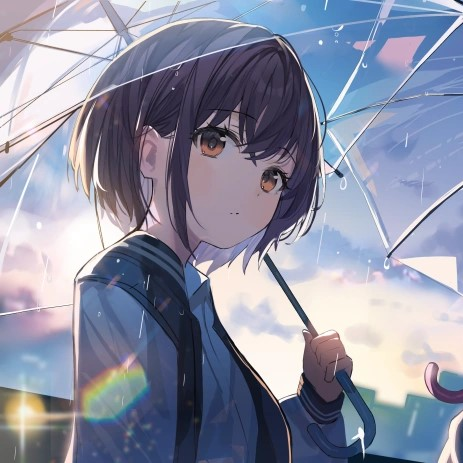
\includegraphics[width=0.67\linewidth]{cover.jpg}\label{fig:coverfigure}
  \end{figure} 
  \vfill
  \large 迷子でもいい、迷子でも進め。                                \\
  \vfill \FandolSong
  二〇二三$\cdot$霜月〇三
\end{center}
\vspace{\stretch{2}}
\end{titlepage}

\tableofcontents

\chapter*{PREFACE}
\iffalse
\begin{figure}[ht]
    \centering
    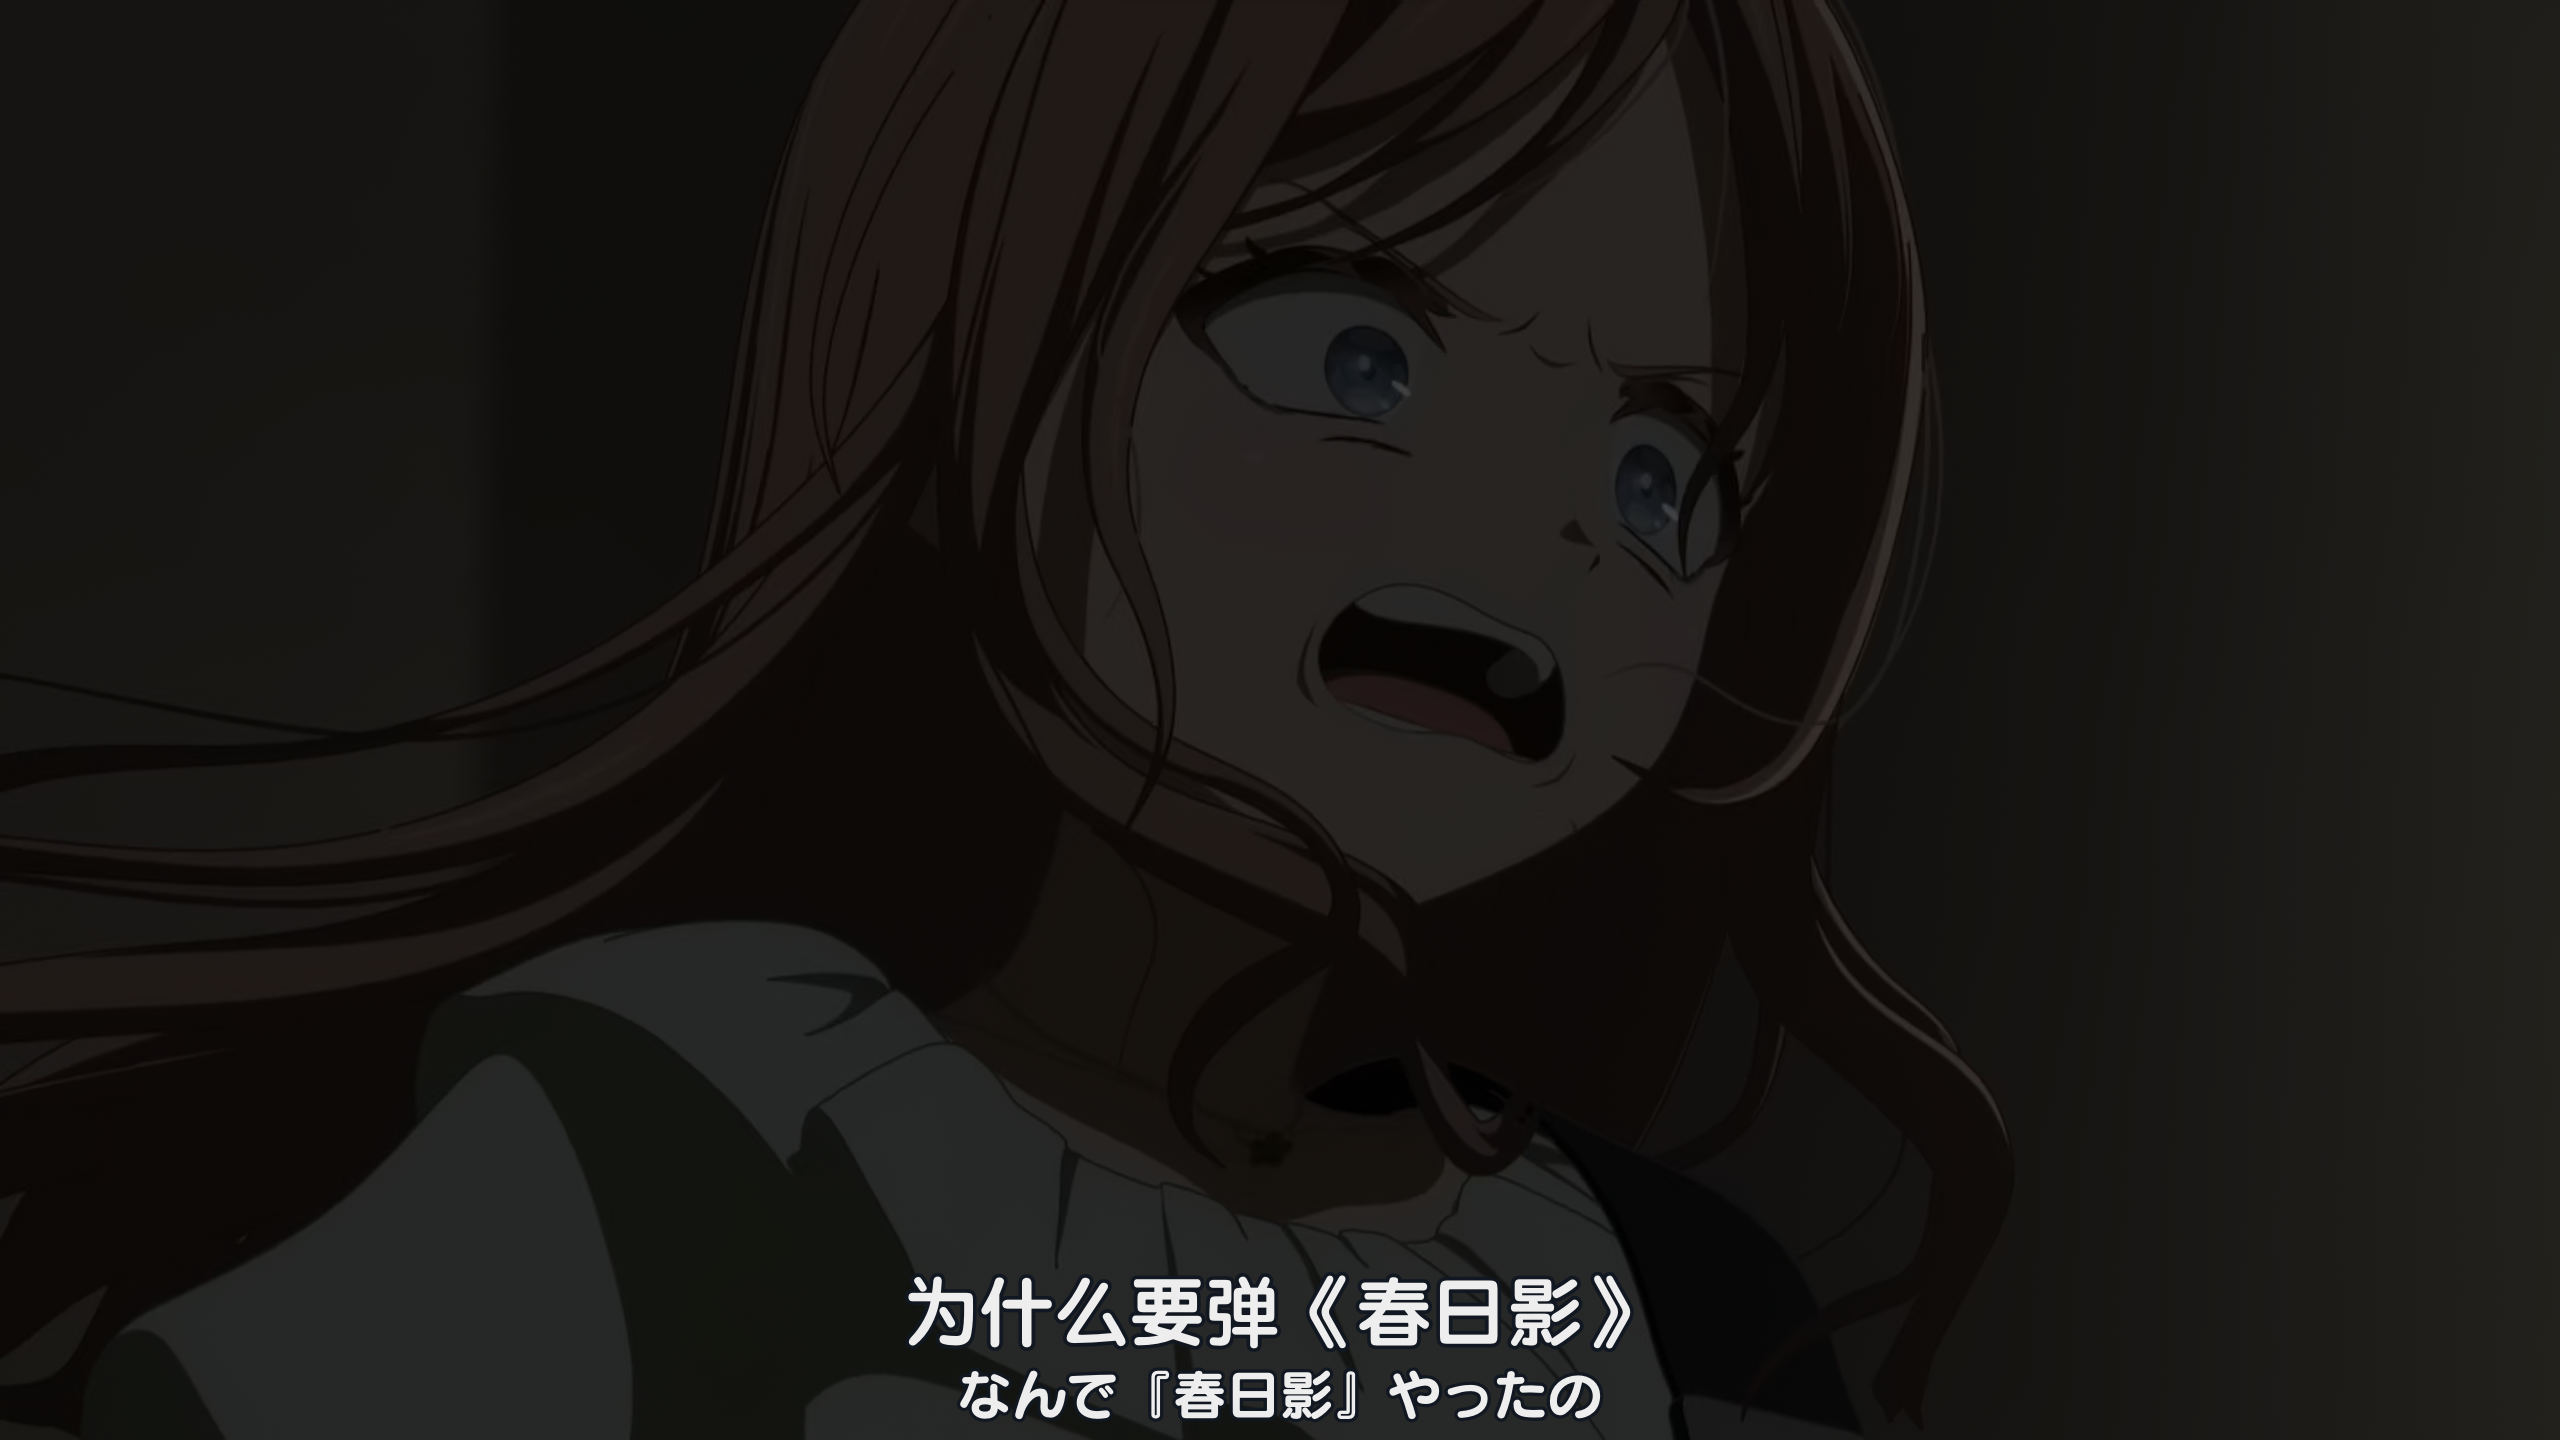
\includegraphics[width=\linewidth]{haruhikage.png}
    %\caption{Caption}
    \label{fig:preface_haruhikage}
\end{figure}
\fi

本note纯属作者自娱自乐(期末复习),仅适用于学过熱力学、統計物理学、量子力学、固体物理学的读者(オタク),\vspace{1ex}
没学完的便乘猫娘
\includegraphics[width=4em,align=c]{idiot.jpg}。
\begin{figure}[ht]
    \centering
    
\includegraphics[width=\linewidth]{teru.png}
    \caption*{teru\ding{73}}
    \label{fig:teru-star}
\end{figure}

\begin{flushright}
	riku\ding{73} \\
	二〇二三$\cdot$師走廿一\\
\end{flushright}



\chapter{半导体中的电子}

\section{半导体的晶格结构与结合性质}

\subsection{金刚石型结构和共价键}

\ce{Si},\ce{Ge}等元素属于IV族元素,外层具有四个价电子。这些元素通过\textbf{共价键}结合形成晶体,晶格结构与\ce{C}元素的金刚石晶体的晶格相同,属于\textbf{金刚石型结构}。这种结构中,每个原子周围有四个近邻原子,组成正四面体结构。这四个原子处于正四面体的顶角上,它们与中心原子各自贡献一个价电子为两个原子共有,并形成共价键。金刚石结构的配位数是$4$。

\begin{figure}[H]
    \centering
\tikzset{every picture/.style={line width=0.75pt}} %set default line width to 0.75pt        

\begin{tikzpicture}[x=0.75pt,y=0.75pt,yscale=-1,xscale=1]
%uncomment if require: \path (0,333); %set diagram left start at 0, and has height of 333

%Flowchart: Extract [id:dp2941884800038894] 
\draw   (279.75,67.58) -- (242.81,261) -- (182.58,191.5) -- cycle ;
%Straight Lines [id:da11678715957846952] 
\draw    (279.75,67.59) -- (379.67,210.72) ;
%Straight Lines [id:da6291753538375728] 
\draw    (242.81,261) -- (379.67,210.72) ;
%Straight Lines [id:da792032373772936] 
\draw  [dash pattern={on 4.5pt off 4.5pt}]  (182.58,191.49) -- (379.67,210.72) ;
%Straight Lines [id:da16681599054483343] 
\draw [color={rgb, 255:red, 0; green, 0; blue, 0 }  ,draw opacity=1 ][fill={rgb, 255:red, 0; green, 0; blue, 0 }  ,fill opacity=1 ]   (281.25,67.64) -- (277.14,172.73)(278.25,67.53) -- (274.14,172.61) ;
%Straight Lines [id:da8617596562201413] 
\draw    (275.94,174.14) -- (182.88,192.96)(275.35,171.2) -- (182.28,190.02) ;
%Straight Lines [id:da5282358800451186] 
\draw    (276.16,171.26) -- (380.18,209.31)(275.13,174.08) -- (379.15,212.13) ;
%Straight Lines [id:da21390436106539057] 
\draw    (277.05,173.19) -- (244.21,261.52)(274.24,172.14) -- (241.4,260.48) ;
%Shape: Circle [id:dp8215196387479993] 
\draw  [fill={rgb, 255:red, 255; green, 255; blue, 255 }  ,fill opacity=1 ] (178.03,191.5) .. controls (178.03,188.98) and (180.07,186.94) .. (182.58,186.94) .. controls (185.1,186.94) and (187.14,188.98) .. (187.14,191.5) .. controls (187.14,194.01) and (185.1,196.05) .. (182.58,196.05) .. controls (180.07,196.05) and (178.03,194.01) .. (178.03,191.5) -- cycle ;
%Shape: Circle [id:dp656158588884858] 
\draw  [fill={rgb, 255:red, 255; green, 255; blue, 255 }  ,fill opacity=1 ] (275.2,67.59) .. controls (275.2,65.07) and (277.24,63.03) .. (279.75,63.03) .. controls (282.27,63.03) and (284.31,65.07) .. (284.31,67.59) .. controls (284.31,70.1) and (282.27,72.14) .. (279.75,72.14) .. controls (277.24,72.14) and (275.2,70.1) .. (275.2,67.59) -- cycle ;
%Shape: Circle [id:dp4448830323802311] 
\draw  [fill={rgb, 255:red, 255; green, 255; blue, 255 }  ,fill opacity=1 ] (375.11,210.72) .. controls (375.11,208.2) and (377.15,206.16) .. (379.67,206.16) .. controls (382.18,206.16) and (384.22,208.2) .. (384.22,210.72) .. controls (384.22,213.23) and (382.18,215.27) .. (379.67,215.27) .. controls (377.15,215.27) and (375.11,213.23) .. (375.11,210.72) -- cycle ;
%Shape: Circle [id:dp8703628065470996] 
\draw  [fill={rgb, 255:red, 255; green, 255; blue, 255 }  ,fill opacity=1 ] (271.09,172.67) .. controls (271.09,170.15) and (273.13,168.11) .. (275.64,168.11) .. controls (278.16,168.11) and (280.2,170.15) .. (280.2,172.67) .. controls (280.2,175.18) and (278.16,177.22) .. (275.64,177.22) .. controls (273.13,177.22) and (271.09,175.18) .. (271.09,172.67) -- cycle ;
%Shape: Circle [id:dp849985969268054] 
\draw  [fill={rgb, 255:red, 255; green, 255; blue, 255 }  ,fill opacity=1 ] (238.25,261) .. controls (238.25,258.48) and (240.29,256.44) .. (242.81,256.44) .. controls (245.32,256.44) and (247.36,258.48) .. (247.36,261) .. controls (247.36,263.52) and (245.32,265.56) .. (242.81,265.56) .. controls (240.29,265.56) and (238.25,263.52) .. (238.25,261) -- cycle ;
\end{tikzpicture}
    \caption{正四面体结构}
    \label{fig:tetrahedron}
\end{figure}

实验测得 \ce{Si}和 \ce{Ge}的晶格常数$a$分别为$0.543102\ \mathrm{nm}$和$0.565791\ \mathrm{nm}$。

\begin{figure}[H]
    \centering
    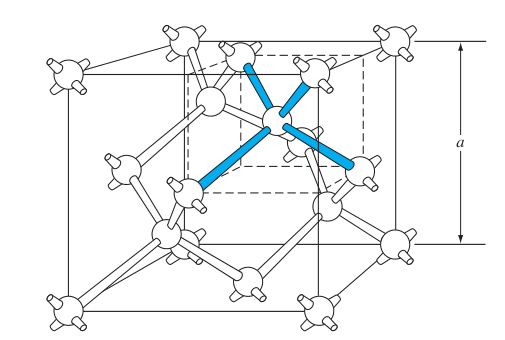
\includegraphics{diamond.png}
    \caption{金刚石晶胞}
    \label{fig:diamond}
\end{figure}

\subsection{闪锌矿型结构和混合键}

III族元素 \ce{Al}, \ce{Ga}, \ce{In}和V族元素 \ce{P}, \ce{As}, \ce{Sb}形成的III-V族化合物是半导体材料,它们具有闪锌矿型结构,这种结构和金刚石结构相似,但它由两种不同的原子组成。这种结构依靠共价键结合,但有一定的离子键成分。

\subsection{纤锌矿型结构}

纤锌矿型结构与闪锌矿型结构类似,以正四面体结构为基础构成,但它具有六方对称性。其结合性质也具有一定的离子性。

\section{半导体中的电子状态和能带}

\subsection{半导体中的电子状态和能带}

晶体中的电子介于孤立原子中的电子和自由电子之间。孤立原子中的电子在原子核和其他电子的势场中运动;自由电子在零势场中运动。

首先介绍自由电子的运动。

微观粒子具有波粒二象性。一个质量$m_0$的自由电子以速度$\bm v$运动,其动量与能量为:
\begin{align}
    &\bm p=m_0 \bm v\label{eq:free_momentum}\\
    &E=\frac{1}{2}\frac{\left|\bm p\right|^2}{m_0}\label{eq:free_energy}
\end{align}

根据波粒二象性,此自由粒子可用频率为$\nu$,角频率$\omega=2\pi\nu$,波长为$\lambda$的自由波函数表示:
\begin{equation}
    \Psi\left(\bm r,\ t\right)=A\mathrm{e}^{\mathrm{i}\left(\bm k\cdot\bm r-\omega t\right)}
\end{equation}
其中,$A$为常数,$\bm k$为波数,规定其为矢量,称为\textbf{波数矢量}或\textbf{波矢},其大小:
\begin{equation}
    k=\left|\bm k\right|=\frac{2\pi}{\lambda}
\end{equation}
方向平行于波面法线,为波的传播方向。

自由电子能量与动量和波的角频率和波矢的关系为:
\begin{align}
    E&=h\nu=\hslash\omega\label{eq:free_energy_wave}\\
    \bm p&=\hslash\bm k\label{eq:free_momentum_wave}
\end{align}
式中,$\hslash=\D\frac{h}{2\pi}$,$h$为普朗克(Planck)常数。

\vspace{1ex}考虑一维情况,选择$Ox$轴方向与波传播方向一致,此时波函数为:
\begin{equation}
    \Psi(x,\ t)=A\mathrm{e}^{\mathrm{i}kx}\mathrm{e}^{-\mathrm{i}\omega t}=\psi(x)\mathrm{e}^{-\mathrm{i}\omega t}
\end{equation}
其中
\begin{equation}
    \psi(x)=A\mathrm{e}^{\mathrm{i}kx}
\end{equation}
称为\textbf{自由电子波函数},它是沿$x$方向传播的平面波,遵循定态薛定谔(Schr\"odinger)方程
\begin{equation}
    -\frac{\hslash^2}{2m_0}\frac{\mathrm{d}^2\psi(x)}
    {\mathrm{d}x^2}=E\psi(x)
\end{equation}

将\autoref{eq:free_momentum_wave}代入\autoref{eq:free_momentum}和\autoref{eq:free_energy}中,得:
\begin{align}
    \bm v&=\frac{\hslash\bm k}{m_0}\label{eq:free_e_wave_velocity}\\
    E&=\frac{\hslash^2k^2}{2m_0}\label{eq:free_e_wave_energy}
\end{align}

对波矢为$\bm k$的运动状态,自由电子能量$E$,动量$\bm p$和速度$\bm v$均确定,故可以用波矢$\bm k$描述自由电子的运动状态。

\begin{figure}[H]
    \centering
\tikzset{every picture/.style={line width=0.75pt}} %set default line width to 0.75pt        

\begin{tikzpicture}[x=0.75pt,y=0.75pt,yscale=-1,xscale=1]
%uncomment if require: \path (0,300); %set diagram left start at 0, and has height of 300

%Shape: Parabola [id:dp9002057271429234] 
\draw   (234.67,67) .. controls (285,223) and (335.33,223) .. (385.67,67) ;
%Shape: Axis 2D [id:dp47011928159342387] 
\draw  (188.17,184) -- (433.17,184)(310.17,57.5) -- (310.17,207.5) (426.17,179) -- (433.17,184) -- (426.17,189) (305.17,64.5) -- (310.17,57.5) -- (315.17,64.5)  ;

% Text Node
\draw (320,53.4) node [anchor=north west][inner sep=0.75pt]    {$E$};
% Text Node
\draw (423,193.4) node [anchor=north west][inner sep=0.75pt]    {$k$};
\end{tikzpicture}
    \caption{自由电子$E-k$曲线}
    \label{fig:free_e_E-k}
\end{figure}

\subsubsection{1. 晶体中薛定谔方程及其解的形式}

单电子近似认为晶体中的电子在与晶格同周期的周期势场中运动。对于一维晶格,$x$处的电势为:
\begin{equation}
    V(x)=V(x+na)\label{eq:cristal_potential}
\end{equation}
其中$n$为整数,$a$为晶格常数。晶体中电子满足薛定谔方程:
\begin{equation}
    -\frac{\hslash^2}{2m_0}\frac{\mathrm{d}^2\psi(x)}{\mathrm{d}x^2}+V(x)\psi(x)=E\psi(x)\label{eq:cristal_schrodinger_eq}
\end{equation}
上式中$V(x)$满足\autoref{eq:cristal_potential}。\autoref{eq:cristal_schrodinger_eq}是晶体电子的基本方程。

可以证明,满足\autoref{eq:cristal_schrodinger_eq}的波函数一定具有如下形式:
\begin{equation}
    \psi_k(x)=u_k(x)\mathrm{e}^{\mathrm{i}kx}\label{eq:bloch_equation}
\end{equation}
式中$k$为波数,$u_k(x)$为与晶格同周期的周期函数:
\begin{equation}
    u_k(x)=u_k(x+na)\quad \text{$n$为整数}
\end{equation}
此结论称为\textbf{布洛赫定理}。具有\autoref{eq:bloch_equation}形式的波函数称为\textbf{布洛赫函数}。

\subsubsection{2. 布里渊区与能带}

晶体中电子处在不同$\bm k$状态,具有不同能量$E(\bm k)$。求解\autoref{eq:cristal_schrodinger_eq}可以得到$E(k)-k$关系曲线。当
\begin{equation}
    k=\frac{n\pi}{a}\quad (n=0,\ \pm 1,\ \pm 2,\cdots)
\end{equation}
时,能量不连续,形成一系列禁带和允带。
\begin{figure}[H]
    \centering
    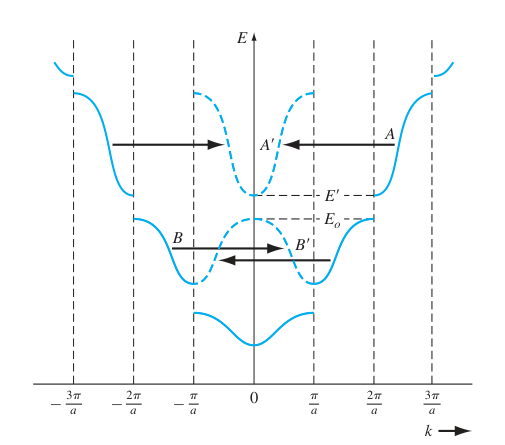
\includegraphics{energy_band.png}
    \caption{$E(k)-k$关系}
    \label{fig:energy_band}
\end{figure}

\vspace{1ex}可以看到,能量$E(k)$也为$k$的周期函数,周期为$\D\frac{2\pi}{a}$:
\begin{equation}
    E(k)=E\left(k+n\frac{2\pi}{a}\right)
\end{equation}
\vspace{1ex}故$k$和$k+\D n\frac{2\pi}{a}$表示相同的状态,可以只取第一布里渊区$\D -\frac{\pi}{a}<k<\frac{\pi}{a}$中的$k$值描述电子的能量状态,
\vspace{1ex}将其他区域移动$\D n\frac{2\pi}{a}$合并到第一区。这个区域内的$E$是$k$的多值函数,我们称此区域为\textbf{简约布里渊区},区域内波矢为\textbf{简约波矢}。

对于有限晶体需要考虑边界条件。根据周期性边界条件,得到波矢$k$只能取分立值。对边长$L$的立方晶体,波矢$\bm k$的各分量:
\begin{equation}
\begin{split}
    k_x=\frac{2\pi n_x}{L}\quad (n_x=0,\ \pm 1,\ \pm 2,\cdots)\\
    k_y=\frac{2\pi n_y}{L}\quad (n_x=0,\ \pm 1,\ \pm 2,\cdots)\\
    k_z=\frac{2\pi n_z}{L}\quad (n_x=0,\ \pm 1,\ \pm 2,\cdots)
\end{split}
\end{equation}

\subsection{导体,半导体,绝缘体}

固体按其导电性分为导体,半导体,绝缘体。

\section{半导体中电子的运动,有效质量}

\subsection{半导体中的\texorpdfstring{$E(k)$}{E(k)}与\texorpdfstring{$k$}{k}的关系}

半导体中起作用的一般是带底或者带顶的电子,因此只要研究带顶和带底附近的$E(k)-k$关系。

我们用泰勒展开近似地研究能带极值附近$E(k)$与$k$的关系。一维情况下,设能带底位于$k=0$处。

将$E(k)$在$k=0$附近泰勒展开,取到$k^2$项:
\begin{equation}
    E(k)=E(0)+\left(\frac{\mathrm{d}E}{\mathrm{d}k}\right)_{k=0}k+\frac{1}{2}\left(\frac{\mathrm{d^2}E}{\mathrm{d}k^2}\right)_{k=0}k^2+\mathcal{O}(k^3)
\end{equation}
\vspace{1ex}由于在$k=0$时,$\D\left(\frac{\mathrm{d}E}{\mathrm{d}k}\right)_{k=0}\propto (\hslash k)_{k=0}=0$,从而:
\begin{equation}
    E(k)-E(0)=\frac{1}{2}\left(\frac{\mathrm{d}^2E}{\mathrm{d}k^2}\right)_{k=0}k^2\label{eq:E(k)-E(0)}
\end{equation}
其中$E(0)$为带底能量。
令
\begin{equation}
    \frac{1}{m_n^*}=\frac{1}{\hslash^2}\left(\frac{\mathrm{d}^2E}{\mathrm{d}k^2}\right)_{k=0}\label{eq:effect_m}
\end{equation}
将\autoref{eq:effect_m}代入\autoref{eq:E(k)-E(0)},得到带底附近$E(k)$为
\begin{equation}
    E(k)-E(0)=\frac{\hslash^2k^2}{2m_n^*}\label{eq:electron_effect_mass_energy_bottom}
\end{equation}
区别于\autoref{eq:free_e_wave_energy}中的电子惯性质量$m_0$,$m_n^*$称为\textbf{带底电子}的\textbf{有效质量}。由于$E(k)>E(0)$,故$m_n^*$是\textbf{正值}。

同样的,设带顶位于$k=0$处,则在带顶附近得到:
\begin{equation}
    E(k)-E(0)=\frac{1}{2}\left(\frac{\mathrm{d^2}E}{\mathrm{d}k^2}\right)_{k=0}k^2
\end{equation}
令
\begin{equation*}
    \frac{1}{m_n^*}=\frac{1}{\hslash^2}\left(\frac{\mathrm{d}^2E}{\mathrm{d}k^2}\right)_{k=0}
\end{equation*}
则带顶附近$E(k)$为
\begin{equation}
    E(k)-E(0)=\frac{\hslash^2k^2}{2m_n^*}\label{eq:electron_effect_mass_energy_top}
\end{equation}
$m_n^*$称为\textbf{带顶电子}的\textbf{有效质量}。由于$E(k)<E(0)$,$m_n^*$为\textbf{负值}。

\autoref{eq:electron_effect_mass_energy_bottom}和\autoref{eq:electron_effect_mass_energy_top}可见,只要能够确定出有效质量$m_n^*$大小,就能得到能带极值附近的$E(k)-k$关系。

\subsection{半导体中电子的平均速度}

\vspace{1ex}自由电子速度由\autoref{eq:free_e_wave_velocity}确定。由\autoref{eq:free_e_wave_energy}可以求得 $\D\frac{\mathrm{d}E}{\mathrm{d}k}=\frac{\hslash^2k}{m_0}$,代入\autoref{eq:free_e_wave_velocity},
\vspace{1ex}得自由电子速度 $\D v=\frac{1}{\hslash}\frac{\mathrm{d}E}{\mathrm{d}k}$。

根据量子力学,电子的运动可以视为波包的运动,波包的群速度即电子的平均速度。设波包由若干角频率$\omega$的波组成,则波包的群速度:
\begin{equation}
    v=\frac{\mathrm{d}\omega}{\mathrm{d}k}\label{eq:wave_group_v}
\end{equation}
又由于角频率$\omega$的波,其粒子能量为$\hslash\omega$,代入\autoref{eq:wave_group_v}:
\begin{equation}
    v=\frac{\mathrm{d}\omega}{\mathrm{d}k}=\frac{1}{\hslash}\frac{\mathrm{d}\hslash\omega}{\mathrm{d}k}=\frac{1}{\hslash}\frac{\mathrm{d}E}{\mathrm{d}k}\label{eq:semi_velocity_energy_relation}
\end{equation}
再代入\autoref{eq:electron_effect_mass_energy_bottom}或\autoref{eq:electron_effect_mass_energy_top},得:
\begin{align}
    v&=\frac{1}{\hslash}\frac{\mathrm{d}}{\mathrm{d}k}\left(E(0)+\frac{\hslash^2k^2}{2m_n^*}\right)\notag\\
    &=\frac{1}{\hslash}\frac{\hslash^2k}{m_n^*}\notag\\
    &=\frac{\hslash k}{m_n^*}\label{eq:semi_velocity_k_m_eff_relation}
\end{align}
带底$m_n^*>0$,$k$为正值时,$v$为正值;带顶$m_n^*《0$,$k$为正值时,$v$为负值

\subsection{半导体中电子的加速度}

在强度$\mathscr{E}$的外电场下,电子受到$f=-q\mathscr{E}$的电场力,$\mathrm{d}t$时间内产生位移$\mathrm{d}s$。外力做功产生的能量变化:
\begin{equation}
    \mathrm{d}E=f\mathrm{d}s=fv\mathrm{d}t
\end{equation}
代入\autoref{eq:semi_velocity_energy_relation},得:
\begin{align}
    &\mathrm{d}E=\frac{f}{\hslash}\frac{\mathrm{d}E}{\mathrm{d}k}\mathrm{d}t\\
    \Longrightarrow&f=\hslash\frac{\mathrm{d}k}{\mathrm{d}t}\label{eq:force_k_t_relation}
\end{align}
上式说明了外力$f$作用下,波矢$k$会发生改变。

电子加速度:
\begin{equation}
    a=\frac{\mathrm{d}v}{\mathrm{d}t}=\frac{1}{\hslash}\frac{\mathrm{d}}{\mathrm{d}t}\frac{\mathrm{d}E}{\mathrm{d}k}=\frac{1}{\hslash}\frac{\mathrm{d}k}{\mathrm{d}t}\frac{\mathrm{d}^2E}{\mathrm{d}k^2}=\frac{f}{\hslash^2}\frac{\mathrm{d}^2E}{\mathrm{d}k^2}
\end{equation}
由
\begin{equation}
    \frac{1}{m_n^*}=\frac{1}{\hslash^2}\frac{\mathrm{d}^2E}{\mathrm{d}k^2}\quad \text{or}\quad m_n^*=\frac{\hslash^2}{\D\frac{\mathrm{d}^2E}{\mathrm{d}k^2}}
\end{equation}
\vspace{1ex}得:
\begin{equation}
    a=\frac{f}{m_n^*}=-\frac{q\mathscr{E}}{m_n^*}
    \label{eq:accel_force}
\end{equation}
可以看出,引入电子有效质量后,半导体电子的运动与牛顿第二定律类似。

\section{本征半导体中的空穴}

在$K=0$下,纯净半导体的价带被价电子填满,导带为空。一定温度下,价带顶部电子被激发到导带。被激发的电子参与导电。价带由于缺少电子,形成带正电的准粒子,即\textbf{空穴}。

空穴具有一个单位的正电荷$+q$,有效质量$m_p^*$有:
\begin{equation}
    m_p^*=-m_n^*
\end{equation}
在外电场$\mathscr{E}$下,空穴的加速度
\begin{equation}
    a=\frac{q\mathscr{E}}{m_p^*}=\frac{f}{m_p^*}
\end{equation}

\chapter{回旋共振与导带和价带结构}

\section{回旋共振}

\subsection{\texorpdfstring{$k$}{k}空间等能面}

根据1.3节,$k=0$在导带底电子,有:
\begin{equation}
    E(k)-E(0)=\frac{\hslash^2k^2}{2m_n^*}
\end{equation}
对于价带顶的空穴,同样有:
\begin{equation}
    E(k)-E(0)=-\frac{\hslash^2k^2}{2m_p^*}
\end{equation}

对于三维晶体,$\bm k$有$k_x,\ k_y,\ k_z$三个分量,满足:
\begin{equation}
    k^2=k_x^2+k_y^2+k_z^2
\end{equation}
代入导带底位于$\bm k=\bm 0$,能量为$E(0)$的情况,有:
\begin{equation}
    E(\bm k)-E(0)=\frac{\hslash^2}{2m_n^*}\left(k_x^2+k_y^2+k_z^2\right)
\end{equation}

对于各向异性的晶体,$E(\bm k)$和$\bm k$的关系在$\bm k$沿不同方向上并不完全一致。

根据
\begin{equation}
    \frac{1}{m_n^*}=\frac{1}{\hslash^2}\frac{\mathrm{d}^2E}{\mathrm{d}\bm k^2}
\end{equation}
\vspace{1ex}可知,$\D\frac{1}{m_n^*}$是一个二阶张量:
\begin{equation}
    \left(\frac{1}{m_n^*}\right)_{ij}=\frac{1}{\hslash^2}\frac{\partial^2E}{\partial k_i\partial k_j},\quad (i,\ j\ \text{取遍}\ 1,\ 2,\ 3)
\end{equation}
\vspace{1ex}我们对$\D\left(\frac{1}{m_n^*}\right)_{ij}$作正交变换,取$\D\left(\frac{1}{m_n^*}\right)_{ij}$仅有对角元素时的基矢为$\bm k_x,\ \bm k_y,\ \bm k_z$。此时记$m_x^*,\ m_y^*,\ m_z^*$分别为$\bm k_x,\ \bm k_y,\ \bm k_z$方向上的电子有效质量:
\begin{equation}
    \left\{
    \begin{aligned}
        \frac{1}{m_x^*}=\frac{1}{\hslash^2}\left(\frac{\partial^2E}{\partial k_x^2}\right)_{k_0}\\
        \frac{1}{m_y^*}=\frac{1}{\hslash^2}\left(\frac{\partial^2E}{\partial k_y^2}\right)_{k_0}\\
        \frac{1}{m_z^*}=\frac{1}{\hslash^2}\left(\frac{\partial^2E}{\partial k_z^2}\right)_{k_0}
        \end{aligned}
    \right.
\end{equation}

设导带底位于$\bm k_0$,能量为$E(k_0)$。在$k_0$附近将$E(k_0)$泰勒展开,取到二次项:
\begin{equation}
    E(k)=E(k_0)+\frac{\hslash^2}{2}\left(\frac{(k_x-k_{0x})^2}{m_x^*}+\frac{(k_y-k_{0y})^2}{m_y^*}+\frac{(k_z-k_{0z})^2}{m_z^*}\right)
    \label{eq:homo_energy_equation}
\end{equation}
即: 
\begin{equation}
    \frac{\quad(k_x-k_{0x})^2\quad}{\D \frac{2m_x^*\left(E-E_c\right)}{\hslash^2}}+
    \frac{\quad(k_y-k_{0y})^2\quad}{\D \frac{2m_y^*\left(E-E_c\right)}{\hslash^2}}+
    \frac{\quad(k_z-k_{0z})^2\quad}{\D \frac{2m_z^*\left(E-E_c\right)}{\hslash^2}}=1
    \label{eq:homo_energy_eclipse_equation}
\end{equation}
\autoref{eq:homo_energy_eclipse_equation}是个椭圆方程,即等能面是围绕$\bm k_0$的一系列椭球面。

\subsection{回旋共振}

半导体置于磁感应强度$\bm B$的磁场中,电子初速度为$\bm v$,磁场力$\bm f$:
\begin{equation}
    \bm f=-q\bm v\times\bm B
\end{equation}
$\bm v$和$\bm B$夹角为$\theta$:
\begin{equation}
    \theta=\arccos{\left(\frac{\bm v\cdot\bm B}{\left|v\right|\left|B\right|}\right)}
\end{equation}
则$f$的大小为:
\begin{equation}
    f=qvB\sin{\theta}=qv_{\perp}B,\quad v_{\perp}=v\sin{\theta}
\end{equation}
电子的轨迹在沿磁场方向为速度$v_{\parallel}=v\cos{\theta}$的匀速运动,在垂直于磁场的平面内作匀速圆周运动,总体的运动轨迹为以螺旋线进动。

设圆周半径$r$,回旋频率为$\omega_c$,则有
\begin{equation}
    v_{\perp}=r\omega_c
\end{equation}
向心加速度$a$:
\begin{equation}
    a=\frac{v_{\perp}^2}{r}
\end{equation}
代入\autoref{eq:accel_force},得
\begin{align}
    &\frac{v_{\perp}^2}{r}=\frac{f}{m_n^{*}}=\frac{qv_{\perp}B}{m_n^*}\notag\\
    \Longrightarrow&v_{\perp}=r\omega_c=\frac{qBr}{m_n^*}\notag\\
    \Longrightarrow&\omega_c=\frac{qB}{m_n^*}\label{eq:ball-cyclotron-resonance}
\end{align}
将电磁波通过半导体样品,当交变电磁场的角频率$\omega$等于回旋频率$\omega_c$时,就会发生共振吸收。测出共振吸收时的电磁波角频率$\omega$和磁感应强度$B$,便可以算出有效质量$m_n$。

若等能面是椭球面,则有效质量也是各向异性的。设沿$k_x,\ k_y,\ k_z$轴方向分别是$m_x^*,\ m_y^*,\ m_z^*$。设$\bm B$沿$k_x,\ k_y,\ k_z$轴的方向余弦为$\alpha,\ \beta,\ \gamma$,则电子受力:
\begin{equation}
\left\{
    \begin{aligned}
        f_x=-qB\left(v_y\gamma-v_z\beta\right)\\
        f_y=-qB\left(v_z\alpha-v_x\gamma\right)\\
        f_z=-qB\left(v_x\beta-v_y\alpha\right)
    \end{aligned}
\right.
\end{equation}
得到运动方程:
\begin{equation}
    \left\{
    \begin{aligned}
        m_x^*\frac{\mathrm{d}v_x}{\mathrm{d}t}+qB\left(v_y\gamma-v_z\beta\right)=0\\
        m_y^*\frac{\mathrm{d}v_y}{\mathrm{d}t}+qB\left(v_z\alpha-v_x\gamma\right)=0\\
        m_z^*\frac{\mathrm{d}v_z}{\mathrm{d}t}+qB\left(v_x\beta-v_y\alpha\right)=0
    \end{aligned}
    \right.
\end{equation}
电子作周期运动,取解:
\begin{equation}
    \left\{
    \begin{aligned}
        v_x=v_x'\mathrm{e}^{\mathrm{i}\omega_ct}\\
        v_y=v_y'\mathrm{e}^{\mathrm{i}\omega_ct}\\
        v_z=v_z'\mathrm{e}^{\mathrm{i}\omega_ct}
    \end{aligned}
    \right.
\end{equation}
代入,得:
\begin{equation}
    \left\{
    \begin{aligned}
        \mathrm{i}\omega_cv_x'+\frac{qB}{m_x^*}\gamma v_y'-\frac{qB}{m_x^*}\beta v_z'=0\\
        -\frac{qB}{m_y^*}\gamma v_x'+\mathrm{i}\omega_cv_y'+\frac{qB}{m_y^*}\alpha v_z'=0\\
        \frac{qB}{m_z^*}\beta v_x'-\frac{qB}{m_z^*}\alpha v_y'+\mathrm{i}\omega_cv_z'=0
    \end{aligned}
    \right.
\end{equation}
要使$v_x',\ v_y',\ v_z'$有不全为零的解,其系数行列式为零:
\begin{equation}
    \begin{vmatrix}
        \mathrm{i}\omega_c & \D\frac{qB}{m_x^*}\gamma & \D-\frac{qB}{m_x^*}\beta\vspace{1ex}\\
        \D-\frac{qB}{m_y^*}\gamma & \mathrm{i}\omega_c & \D\frac{qB}{m_y^*}\alpha\vspace{1ex}\\
        \D\frac{qB}{m_z^*}\beta & \D-\frac{qB}{m_z^*}\alpha & \mathrm{i}\omega_c
    \end{vmatrix}
    =0
\end{equation}
解得电子回旋频率$\omega_c$:
\begin{equation}
    \omega_c=\frac{qB}{m_n^*}
\end{equation}
其中
\begin{equation}
    \frac{1}{m_n^*}=\sqrt{\frac{m_x^*\alpha^2+m_y^*\beta^2+m_z^*\gamma^2}{m_x^*m_y^*m_z^*}}\label{eq:ecllipse-cyclotron-resonance-eff-mass}
\end{equation}
交变电磁场的角频率$\omega$等于$\omega_c$时,发生共振吸收。

\section{硅和锗的能带结构}

\subsection{硅和锗的导带结构}

对于等能面为球面的晶体,由\autoref{eq:ball-cyclotron-resonance},改变磁场方向仅有一个吸收峰。硅的回旋共振实验中:
\begin{enumerate}[(1)]
    \item $\bm B$沿$[1\ 1\ 1]$方向,有一个吸收峰;
    \item $\bm B$沿$[1\ 1\ 0]$方向,有两个吸收峰;
    \item $\bm B$沿$[1\ 0\ 0]$方向,有两个吸收峰;
    \item $\bm B$沿任意取向,有三个吸收峰。
\end{enumerate}
显然不是各向同性的。我们认为硅导带底附近等能面是沿$[1\ 0\ 0]$方向的旋转椭球面,且椭圆长轴沿此方向,则与实验事实吻合。此时的导带最小值不在$\bm k$空间原点,而在$[1\ 0\ 0]$方向上,根据对称性,也出现在$[\Bar{1}\ 0\ 0],\ [0\ 1\ 0],\ [0\ \Bar{1},\ 0],\ [0\ 0\ 1],\ [0\ 0\ \Bar{1}]$方向上,如\autoref{fig:homo-energy-phase}。
\begin{figure}[H]
    \centering
\tikzset{every picture/.style={line width=0.75pt}} %set default line width to 0.75pt        

\begin{tikzpicture}[x=0.75pt,y=0.75pt,yscale=-1,xscale=1]
%uncomment if require: \path (0,300); %set diagram left start at 0, and has height of 300

%Straight Lines [id:da22604722746412387] 
\draw    (264.67,259.75) -- (264.7,49.75) ;
\draw [shift={(264.7,49.75)}, rotate = 270.01] [color={rgb, 255:red, 0; green, 0; blue, 0 }  ][fill={rgb, 255:red, 0; green, 0; blue, 0 }  ][line width=0.75]      (0, 0) circle [x radius= 3.35, y radius= 3.35]   ;
\draw [shift={(264.67,259.75)}, rotate = 270.01] [color={rgb, 255:red, 0; green, 0; blue, 0 }  ][fill={rgb, 255:red, 0; green, 0; blue, 0 }  ][line width=0.75]      (0, 0) circle [x radius= 3.35, y radius= 3.35]   ;
%Straight Lines [id:da7464742627624705] 
\draw    (135.17,154.75) -- (392.17,154.75) ;
\draw [shift={(392.17,154.75)}, rotate = 0] [color={rgb, 255:red, 0; green, 0; blue, 0 }  ][fill={rgb, 255:red, 0; green, 0; blue, 0 }  ][line width=0.75]      (0, 0) circle [x radius= 3.35, y radius= 3.35]   ;
\draw [shift={(135.17,154.75)}, rotate = 0] [color={rgb, 255:red, 0; green, 0; blue, 0 }  ][fill={rgb, 255:red, 0; green, 0; blue, 0 }  ][line width=0.75]      (0, 0) circle [x radius= 3.35, y radius= 3.35]   ;
%Straight Lines [id:da8922617180358392] 
\draw    (174.67,235.75) -- (351.17,77.75) ;
\draw [shift={(351.17,77.75)}, rotate = 318.17] [color={rgb, 255:red, 0; green, 0; blue, 0 }  ][fill={rgb, 255:red, 0; green, 0; blue, 0 }  ][line width=0.75]      (0, 0) circle [x radius= 3.35, y radius= 3.35]   ;
\draw [shift={(174.67,235.75)}, rotate = 318.17] [color={rgb, 255:red, 0; green, 0; blue, 0 }  ][fill={rgb, 255:red, 0; green, 0; blue, 0 }  ][line width=0.75]      (0, 0) circle [x radius= 3.35, y radius= 3.35]   ;
%Shape: Ellipse [id:dp14232987209042292] 
\draw  [fill={rgb, 255:red, 80; green, 227; blue, 194 }  ,fill opacity=1 ] (187.9,224) .. controls (184.14,219.8) and (189.25,209.07) .. (199.32,200.04) .. controls (209.39,191) and (220.61,187.08) .. (224.37,191.27) .. controls (228.14,195.47) and (223.03,206.2) .. (212.95,215.23) .. controls (202.88,224.27) and (191.67,228.19) .. (187.9,224) -- cycle ;
%Shape: Ellipse [id:dp5560073327977961] 
\draw  [fill={rgb, 255:red, 80; green, 227; blue, 194 }  ,fill opacity=1 ] (302.9,120.5) .. controls (299.14,116.3) and (304.25,105.57) .. (314.32,96.54) .. controls (324.39,87.5) and (335.61,83.58) .. (339.37,87.77) .. controls (343.14,91.97) and (338.03,102.7) .. (327.95,111.73) .. controls (317.88,120.77) and (306.67,124.69) .. (302.9,120.5) -- cycle ;
%Shape: Ellipse [id:dp7111731340388567] 
\draw  [fill={rgb, 255:red, 80; green, 227; blue, 194 }  ,fill opacity=1 ] (335.14,155.27) .. controls (335.11,149.63) and (346.05,145) .. (359.58,144.93) .. controls (373.11,144.85) and (384.11,149.36) .. (384.14,155) .. controls (384.17,160.64) and (373.22,165.27) .. (359.69,165.34) .. controls (346.16,165.42) and (335.17,160.91) .. (335.14,155.27) -- cycle ;
%Shape: Ellipse [id:dp8131792583845494] 
\draw  [fill={rgb, 255:red, 80; green, 227; blue, 194 }  ,fill opacity=1 ] (146.14,154.77) .. controls (146.11,149.13) and (157.05,144.5) .. (170.58,144.43) .. controls (184.11,144.35) and (195.11,148.86) .. (195.14,154.5) .. controls (195.17,160.14) and (184.22,164.77) .. (170.69,164.84) .. controls (157.16,164.92) and (146.17,160.41) .. (146.14,154.77) -- cycle ;
%Shape: Ellipse [id:dp3883439769649071] 
\draw  [fill={rgb, 255:red, 80; green, 227; blue, 194 }  ,fill opacity=1 ] (264.45,59.64) .. controls (270.09,59.59) and (274.74,70.53) .. (274.85,84.06) .. controls (274.95,97.59) and (270.46,108.59) .. (264.82,108.63) .. controls (259.18,108.68) and (254.53,97.74) .. (254.43,84.21) .. controls (254.33,70.68) and (258.82,59.68) .. (264.45,59.64) -- cycle ;
%Shape: Ellipse [id:dp974977775233371] 
\draw  [fill={rgb, 255:red, 80; green, 227; blue, 194 }  ,fill opacity=1 ] (264.45,200.64) .. controls (270.09,200.59) and (274.74,211.53) .. (274.85,225.06) .. controls (274.95,238.59) and (270.46,249.59) .. (264.82,249.63) .. controls (259.18,249.68) and (254.53,238.74) .. (254.43,225.21) .. controls (254.33,211.68) and (258.82,200.68) .. (264.45,200.64) -- cycle ;

% Text Node
\draw (240.17,25.23) node [anchor=north west][inner sep=0.75pt]    {$[ 0\ 0\ 1]$};
% Text Node
\draw (241.67,265.73) node [anchor=north west][inner sep=0.75pt]    {$[ 0\ 0\ \overline{1}]$};
% Text Node
\draw (400.67,146.23) node [anchor=north west][inner sep=0.75pt]    {$[ 0\ 1\ 0]$};
% Text Node
\draw (78.67,141.73) node [anchor=north west][inner sep=0.75pt]    {$[ 0\ \overline{1} \ 0]$};
% Text Node
\draw (356.67,55.73) node [anchor=north west][inner sep=0.75pt]    {$[ \overline{1}\ 0\ 0]$};
% Text Node
\draw (124.17,237.23) node [anchor=north west][inner sep=0.75pt]    {$[1 \ 0\ 0]$};
\end{tikzpicture}
    \caption{硅导带等能面}
    \label{fig:homo-energy-phase}
\end{figure}

由\autoref{eq:homo_energy_equation},极值附近能量$E^s(\bm k)$为:
\begin{equation}
    E^s(\bm k)=E_c+\frac{\hslash^2}{2}\left(\frac{(k_x-k_{0x}^s)^2}{m_x^*}+\frac{(k_y-k_{0y}^s)^2}{m_y^*}+\frac{(k_z-k_{0z}^s)^2}{m_z^*}\right)
\end{equation}

取$E_c$为能量零点,$\bm k_0^s$为坐标原点,取$k_1,\ k_2,\ k_3$三个直角坐标轴分别沿椭球主轴方向,其中$k_3$沿长轴方向$(<100>)$,等能面为绕$k_3$的旋转椭球面。此时沿$k_1,\ k_2$轴的有效质量相同,如\autoref{fig:k-space-B}。

令$m_x^*=m_y^*=m_t$为\textbf{横向有效质量},$m_z^*=m_l$为\textbf{纵向有效质量}。等能面方程化为:
\begin{equation}
    E(\bm k)=\frac{\hslash^2}{2}\left[\frac{k_1^2+k_2^2}{m_t}+\frac{k_3^2}{m_l}\right]
\end{equation}
\begin{figure}[ht]
    \centering
\tikzset{every picture/.style={line width=0.75pt}} %set default line width to 0.75pt        

\begin{tikzpicture}[x=0.75pt,y=0.75pt,yscale=-1,xscale=1]
%uncomment if require: \path (0,300); %set diagram left start at 0, and has height of 300

%Shape: Axis 2D [id:dp8786621681916096] 
\draw  (260.67,136.08) -- (361.17,136.08)(260.67,43.08) -- (260.67,136.08) -- cycle (354.17,131.08) -- (361.17,136.08) -- (354.17,141.08) (255.67,50.08) -- (260.67,43.08) -- (265.67,50.08)  ;
%Straight Lines [id:da8481261784727727] 
\draw    (260.67,136.08) -- (207.09,188.68) ;
\draw [shift={(205.67,190.08)}, rotate = 315.53] [color={rgb, 255:red, 0; green, 0; blue, 0 }  ][line width=0.75]    (10.93,-4.9) .. controls (6.95,-2.3) and (3.31,-0.67) .. (0,0) .. controls (3.31,0.67) and (6.95,2.3) .. (10.93,4.9)   ;
\draw [shift={(260.67,136.08)}, rotate = 135.53] [color={rgb, 255:red, 0; green, 0; blue, 0 }  ][fill={rgb, 255:red, 0; green, 0; blue, 0 }  ][line width=0.75]      (0, 0) circle [x radius= 3.35, y radius= 3.35]   ;
%Shape: Ellipse [id:dp9193111334407007] 
\draw   (260.67,101.08) .. controls (271.71,101.08) and (280.67,116.75) .. (280.67,136.08) .. controls (280.67,155.41) and (271.71,171.08) .. (260.67,171.08) .. controls (249.62,171.08) and (240.67,155.41) .. (240.67,136.08) .. controls (240.67,116.75) and (249.62,101.08) .. (260.67,101.08) -- cycle ;
%Shape: Ellipse [id:dp9104121259221969] 
\draw   (240.67,136.08) .. controls (240.67,130.26) and (249.62,125.54) .. (260.67,125.54) .. controls (271.71,125.54) and (280.67,130.26) .. (280.67,136.08) .. controls (280.67,141.91) and (271.71,146.62) .. (260.67,146.62) .. controls (249.62,146.62) and (240.67,141.91) .. (240.67,136.08) -- cycle ;
%Straight Lines [id:da5005870637429592] 
\draw    (260.67,136.08) -- (182.76,77.29) ;
\draw [shift={(181.17,76.08)}, rotate = 37.04] [color={rgb, 255:red, 0; green, 0; blue, 0 }  ][line width=0.75]    (10.93,-3.29) .. controls (6.95,-1.4) and (3.31,-0.3) .. (0,0) .. controls (3.31,0.3) and (6.95,1.4) .. (10.93,3.29)   ;
%Curve Lines [id:da2319691018502339] 
\draw    (228.2,108.32) .. controls (233.34,100.54) and (245.58,92.11) .. (257.72,91.95) ;
\draw [shift={(260.67,92.08)}, rotate = 185.91] [fill={rgb, 255:red, 0; green, 0; blue, 0 }  ][line width=0.08]  [draw opacity=0] (10.72,-5.15) -- (0,0) -- (10.72,5.15) -- (7.12,0) -- cycle    ;
\draw [shift={(226.67,111.08)}, rotate = 293.96] [fill={rgb, 255:red, 0; green, 0; blue, 0 }  ][line width=0.08]  [draw opacity=0] (10.72,-5.15) -- (0,0) -- (10.72,5.15) -- (7.12,0) -- cycle    ;

% Text Node
\draw (212.17,192.4) node [anchor=north west][inner sep=0.75pt]    {$k_{1}$};
% Text Node
\draw (346.67,141.9) node [anchor=north west][inner sep=0.75pt]    {$k_{2}$};
% Text Node
\draw (266.67,37.4) node [anchor=north west][inner sep=0.75pt]    {$k_{3}$};
% Text Node
\draw (224.67,20.9) node [anchor=north west][inner sep=0.75pt]    {$< 100 >$};
% Text Node
\draw (175.17,56.4) node [anchor=north west][inner sep=0.75pt]    {$\bm B $};
% Text Node
\draw (230.17,79.4) node [anchor=north west][inner sep=0.75pt]    {$\theta $};
% Text Node
\draw (254.67,140.9) node [anchor=north west][inner sep=0.75pt]    {$O$};
\end{tikzpicture}
    \caption{$\bm k$空间取向}
    \label{fig:k-space-B}
\end{figure}

我们选取$k_1$使得$\bm B$位于$k_1$和$k_3$组成的平面内,并与$k_3$成$\theta$角。此时$\bm B$的方向余弦:
\begin{equation}
    \alpha=\sin\theta,\ \beta=0,\ \gamma=\cos\theta
\end{equation}
代入\autoref{eq:ecllipse-cyclotron-resonance-eff-mass},得:
\begin{equation}
    m_n^*=m_t\sqrt{\frac{m_l}{m_t\sin^2\theta+m_l\cos^2\theta}}\label{eq:silicon-cyclotron-resonance-eff-mass}
\end{equation}

\begin{enumerate}[(1)]
    \item \vspace{1ex}当$\bm B$沿$[1\ 1\ 1]$方向,则与$6$个$<100>$方向夹角均为$\cos^2\theta=\D\frac{1}{3}$,因此$\sin^2\theta=\D\frac{2}{3}$,代入\autoref{eq:silicon-cyclotron-resonance-eff-mass},得:
    \begin{equation}
        m_n^*=m_t\sqrt{\frac{3m_l}{2m_t+m_l}}
    \end{equation}
    \vspace{1ex}由$\omega=\omega_c=\D\frac{qB}{m_n^*}$可知,$m_n^*$只有一个值,只能观察到一个吸收峰。
    \item $\bm B$沿$[1\ 1\ 0]$方向,此时$\bm B$与$[1\ 0\ 0],\ [\overline{1}\ 0\ 0],\ [0\ 1\ 0],\ [0,\ \overline{1},\ 0]$夹角$\cos^2\theta_1=\D\frac{1}{2},\ \sin^2\theta_1=\D\frac{1}{2}$,与$[0\ 0\ 1],\ [0\ 0\ \overline{1}]$夹角有$\cos^2\theta_2=0,\ \sin^2\theta_2=1$,代入\autoref{eq:silicon-cyclotron-resonance-eff-mass},相应的有效质量分别为:
    \begin{align}
        m_{n1}^*&=m_t\sqrt{\frac{2m_l}{m_t+m_l}}\\
        m_{n2}^*&=\sqrt{m_lm_t}
    \end{align}
    存在$2$个不同的$m_n^*$值,故有两个吸收峰。
    \item $\bm B$沿$[1\ 0\ 0]$方向,此时$\bm B$与$[1\ 0\ 0],\ [\overline{1}\ 0\ 0]$夹角给出$\cos^2\theta_1=1,\ \sin^2\theta_=0$,
    与
    $[0\ 1\ 0]$
    ,\ $[0,\ \overline{1},\ 0]$
    ,\ $[0\ 0\ 1]$
    ,\ $[0\ 0\ \overline{1}]$
    夹角有$\cos^2\theta_2=0,\ \sin^2\theta_2=1$。代入\autoref{eq:silicon-cyclotron-resonance-eff-mass},相应的有效质量分别为:
    \begin{align}
        m_n^*&=m_t\\
        m_n^*&=\sqrt{m_lm_t}
    \end{align}
    存在$2$个不同的$m_n^*$值,故也有两个吸收峰。
    \item $\bm B$沿任意方向时,与$<100>$夹角给出三种$\cos^2\theta$值,因此有三种不同的$m_n^*$,可以观察到三个吸收峰。
\end{enumerate}
上述讨论与实验结果相符,因此硅导带底附近等能面是沿$[1\ 0\ 0]$方向的旋转椭球面。

对于n型锗的实验结果显示,锗的导带极值位于$<111>$方向。
























\chapter{半导体中的杂质和和缺陷能级}

\section{Si、Ge晶体中的杂质能级}

\subsection{替位式杂质和间隙式杂质}

杂质进入半导体后只能以两种方式存在,一种是杂质原子位于晶格原子间的间隙位置,称为\textbf{间隙式杂质},另一种是杂质原子取代晶格原子位于晶格点处,称为\textbf{替位式杂质}。

间隙式杂质原子一般比较小,如 $\ce{Li+}$半径很小($0.068\ \mathrm{nm}$),在$\ce{Si},\ \ce{Ge},\ \ce{AsGa}$中是间隙式杂质。

形成替位式杂质时,要求杂质原子的大小与被取代的晶格原子大小相近,价电子壳层结构相近。如III、V族元素在IV族半导体元素晶体(Si、Ge)中形成替位式杂质。

单位体积杂质原子数称为\textbf{杂质浓度},通常用于表示半导体晶体杂质含量。

\subsection{施主杂质、施主能级} 

III、V族元素在Si、Ge晶体中形成替位式杂质。

在如\autoref{fig:Ge-As}所示的替位杂质中:
\begin{figure}[ht]
    \centering
        
\tikzset{every picture/.style={line width=0.75pt}} %set default line width to 0.75pt        

\begin{tikzpicture}[x=0.75pt,y=0.75pt,yscale=-1,xscale=1]
%uncomment if require: \path (0,395); %set diagram left start at 0, and has height of 395

%Shape: Grid [id:dp6807270511623922] 
\draw  [draw opacity=0] (310.17,58.08) -- (453.42,208.89) -- (302.62,352.14) -- (159.36,201.34) -- cycle ; \draw   (345.98,95.78) -- (195.18,239.04)(381.8,133.48) -- (230.99,276.74)(417.61,171.19) -- (266.81,314.44) ; \draw   (272.47,93.9) -- (415.72,244.7)(234.77,129.71) -- (378.02,280.51)(197.06,165.53) -- (340.32,316.33) ; \draw   (310.17,58.08) -- (453.42,208.89) -- (302.62,352.14) -- (159.36,201.34) -- cycle ;
%Shape: Circle [id:dp046063409388742205] 
\draw  [fill={rgb, 255:red, 255; green, 255; blue, 255 }  ,fill opacity=1 ] (143.86,201.34) .. controls (143.86,192.78) and (150.8,185.84) .. (159.36,185.84) .. controls (167.92,185.84) and (174.86,192.78) .. (174.86,201.34) .. controls (174.86,209.9) and (167.92,216.84) .. (159.36,216.84) .. controls (150.8,216.84) and (143.86,209.9) .. (143.86,201.34) -- cycle ;
%Shape: Circle [id:dp5598570457933985] 
\draw  [fill={rgb, 255:red, 255; green, 255; blue, 255 }  ,fill opacity=1 ] (181.56,165.53) .. controls (181.56,156.97) and (188.5,150.03) .. (197.06,150.03) .. controls (205.62,150.03) and (212.56,156.97) .. (212.56,165.53) .. controls (212.56,174.09) and (205.62,181.03) .. (197.06,181.03) .. controls (188.5,181.03) and (181.56,174.09) .. (181.56,165.53) -- cycle ;
%Shape: Circle [id:dp029451512819909986] 
\draw  [fill={rgb, 255:red, 255; green, 255; blue, 255 }  ,fill opacity=1 ] (219.27,129.71) .. controls (219.27,121.15) and (226.2,114.21) .. (234.77,114.21) .. controls (243.33,114.21) and (250.27,121.15) .. (250.27,129.71) .. controls (250.27,138.27) and (243.33,145.21) .. (234.77,145.21) .. controls (226.2,145.21) and (219.27,138.27) .. (219.27,129.71) -- cycle ;
%Shape: Circle [id:dp5621215056634463] 
\draw  [fill={rgb, 255:red, 255; green, 255; blue, 255 }  ,fill opacity=1 ] (256.97,93.9) .. controls (256.97,85.34) and (263.91,78.4) .. (272.47,78.4) .. controls (281.03,78.4) and (287.97,85.34) .. (287.97,93.9) .. controls (287.97,102.46) and (281.03,109.4) .. (272.47,109.4) .. controls (263.91,109.4) and (256.97,102.46) .. (256.97,93.9) -- cycle ;
%Shape: Circle [id:dp6150691897565472] 
\draw  [fill={rgb, 255:red, 255; green, 255; blue, 255 }  ,fill opacity=1 ] (294.67,58.08) .. controls (294.67,49.52) and (301.61,42.58) .. (310.17,42.58) .. controls (318.73,42.58) and (325.67,49.52) .. (325.67,58.08) .. controls (325.67,66.64) and (318.73,73.58) .. (310.17,73.58) .. controls (301.61,73.58) and (294.67,66.64) .. (294.67,58.08) -- cycle ;
%Shape: Circle [id:dp9834237495398297] 
\draw  [fill={rgb, 255:red, 255; green, 255; blue, 255 }  ,fill opacity=1 ] (330.48,95.78) .. controls (330.48,87.22) and (337.42,80.28) .. (345.98,80.28) .. controls (354.54,80.28) and (361.48,87.22) .. (361.48,95.78) .. controls (361.48,104.34) and (354.54,111.28) .. (345.98,111.28) .. controls (337.42,111.28) and (330.48,104.34) .. (330.48,95.78) -- cycle ;
%Shape: Circle [id:dp4811696109046164] 
\draw  [fill={rgb, 255:red, 255; green, 255; blue, 255 }  ,fill opacity=1 ] (366.3,133.48) .. controls (366.3,124.92) and (373.23,117.98) .. (381.8,117.98) .. controls (390.36,117.98) and (397.3,124.92) .. (397.3,133.48) .. controls (397.3,142.05) and (390.36,148.98) .. (381.8,148.98) .. controls (373.23,148.98) and (366.3,142.05) .. (366.3,133.48) -- cycle ;
%Shape: Circle [id:dp31716452119112226] 
\draw  [fill={rgb, 255:red, 255; green, 255; blue, 255 }  ,fill opacity=1 ] (402.11,171.19) .. controls (402.11,162.63) and (409.05,155.69) .. (417.61,155.69) .. controls (426.17,155.69) and (433.11,162.63) .. (433.11,171.19) .. controls (433.11,179.75) and (426.17,186.69) .. (417.61,186.69) .. controls (409.05,186.69) and (402.11,179.75) .. (402.11,171.19) -- cycle ;
%Shape: Circle [id:dp9746450120900616] 
\draw  [fill={rgb, 255:red, 255; green, 255; blue, 255 }  ,fill opacity=1 ] (437.92,208.89) .. controls (437.92,200.33) and (444.86,193.39) .. (453.42,193.39) .. controls (461.98,193.39) and (468.92,200.33) .. (468.92,208.89) .. controls (468.92,217.45) and (461.98,224.39) .. (453.42,224.39) .. controls (444.86,224.39) and (437.92,217.45) .. (437.92,208.89) -- cycle ;
%Shape: Circle [id:dp6515111127767084] 
\draw  [fill={rgb, 255:red, 255; green, 255; blue, 255 }  ,fill opacity=1 ] (292.78,131.6) .. controls (292.78,123.04) and (299.72,116.1) .. (308.28,116.1) .. controls (316.84,116.1) and (323.78,123.04) .. (323.78,131.6) .. controls (323.78,140.16) and (316.84,147.1) .. (308.28,147.1) .. controls (299.72,147.1) and (292.78,140.16) .. (292.78,131.6) -- cycle ;
%Shape: Circle [id:dp4071487594121945] 
\draw  [fill={rgb, 255:red, 255; green, 255; blue, 255 }  ,fill opacity=1 ] (255.08,167.41) .. controls (255.08,158.85) and (262.02,151.91) .. (270.58,151.91) .. controls (279.14,151.91) and (286.08,158.85) .. (286.08,167.41) .. controls (286.08,175.97) and (279.14,182.91) .. (270.58,182.91) .. controls (262.02,182.91) and (255.08,175.97) .. (255.08,167.41) -- cycle ;
%Shape: Circle [id:dp45799565687287735] 
\draw  [fill={rgb, 255:red, 255; green, 255; blue, 255 }  ,fill opacity=1 ] (217.38,203.23) .. controls (217.38,194.67) and (224.32,187.73) .. (232.88,187.73) .. controls (241.44,187.73) and (248.38,194.67) .. (248.38,203.23) .. controls (248.38,211.79) and (241.44,218.73) .. (232.88,218.73) .. controls (224.32,218.73) and (217.38,211.79) .. (217.38,203.23) -- cycle ;
%Shape: Circle [id:dp44147154664981914] 
\draw  [fill={rgb, 255:red, 255; green, 255; blue, 255 }  ,fill opacity=1 ] (179.68,239.04) .. controls (179.68,230.48) and (186.62,223.54) .. (195.18,223.54) .. controls (203.74,223.54) and (210.68,230.48) .. (210.68,239.04) .. controls (210.68,247.6) and (203.74,254.54) .. (195.18,254.54) .. controls (186.62,254.54) and (179.68,247.6) .. (179.68,239.04) -- cycle ;
%Shape: Circle [id:dp9717781572552524] 
\draw  [fill={rgb, 255:red, 255; green, 255; blue, 255 }  ,fill opacity=1 ] (328.59,169.3) .. controls (328.59,160.74) and (335.53,153.8) .. (344.09,153.8) .. controls (352.65,153.8) and (359.59,160.74) .. (359.59,169.3) .. controls (359.59,177.86) and (352.65,184.8) .. (344.09,184.8) .. controls (335.53,184.8) and (328.59,177.86) .. (328.59,169.3) -- cycle ;
%Shape: Circle [id:dp6132423641852609] 
\draw  [fill={rgb, 255:red, 255; green, 255; blue, 255 }  ,fill opacity=1 ] (290.89,205.11) .. controls (290.89,196.55) and (297.83,189.61) .. (306.39,189.61) .. controls (314.95,189.61) and (321.89,196.55) .. (321.89,205.11) .. controls (321.89,213.67) and (314.95,220.61) .. (306.39,220.61) .. controls (297.83,220.61) and (290.89,213.67) .. (290.89,205.11) -- cycle ;
%Shape: Circle [id:dp4060994688976116] 
\draw  [fill={rgb, 255:red, 255; green, 255; blue, 255 }  ,fill opacity=1 ] (253.19,240.93) .. controls (253.19,232.37) and (260.13,225.43) .. (268.69,225.43) .. controls (277.25,225.43) and (284.19,232.37) .. (284.19,240.93) .. controls (284.19,249.49) and (277.25,256.43) .. (268.69,256.43) .. controls (260.13,256.43) and (253.19,249.49) .. (253.19,240.93) -- cycle ;
%Shape: Circle [id:dp11978777626960158] 
\draw  [fill={rgb, 255:red, 255; green, 255; blue, 255 }  ,fill opacity=1 ] (215.49,276.74) .. controls (215.49,268.18) and (222.43,261.24) .. (230.99,261.24) .. controls (239.55,261.24) and (246.49,268.18) .. (246.49,276.74) .. controls (246.49,285.3) and (239.55,292.24) .. (230.99,292.24) .. controls (222.43,292.24) and (215.49,285.3) .. (215.49,276.74) -- cycle ;
%Shape: Circle [id:dp5173906070930463] 
\draw  [fill={rgb, 255:red, 255; green, 255; blue, 255 }  ,fill opacity=1 ] (364.41,207) .. controls (364.41,198.44) and (371.35,191.5) .. (379.91,191.5) .. controls (388.47,191.5) and (395.41,198.44) .. (395.41,207) .. controls (395.41,215.56) and (388.47,222.5) .. (379.91,222.5) .. controls (371.35,222.5) and (364.41,215.56) .. (364.41,207) -- cycle ;
%Shape: Circle [id:dp7739940881746801] 
\draw  [fill={rgb, 255:red, 255; green, 255; blue, 255 }  ,fill opacity=1 ] (326.71,242.81) .. controls (326.71,234.25) and (333.65,227.31) .. (342.21,227.31) .. controls (350.77,227.31) and (357.71,234.25) .. (357.71,242.81) .. controls (357.71,251.37) and (350.77,258.31) .. (342.21,258.31) .. controls (333.65,258.31) and (326.71,251.37) .. (326.71,242.81) -- cycle ;
%Shape: Circle [id:dp9485458234171835] 
\draw  [fill={rgb, 255:red, 255; green, 255; blue, 255 }  ,fill opacity=1 ] (289.01,278.63) .. controls (289.01,270.07) and (295.95,263.13) .. (304.51,263.13) .. controls (313.07,263.13) and (320.01,270.07) .. (320.01,278.63) .. controls (320.01,287.19) and (313.07,294.13) .. (304.51,294.13) .. controls (295.95,294.13) and (289.01,287.19) .. (289.01,278.63) -- cycle ;
%Shape: Circle [id:dp44553437052240064] 
\draw  [fill={rgb, 255:red, 255; green, 255; blue, 255 }  ,fill opacity=1 ] (251.31,314.44) .. controls (251.31,305.88) and (258.25,298.94) .. (266.81,298.94) .. controls (275.37,298.94) and (282.31,305.88) .. (282.31,314.44) .. controls (282.31,323) and (275.37,329.94) .. (266.81,329.94) .. controls (258.25,329.94) and (251.31,323) .. (251.31,314.44) -- cycle ;
%Shape: Circle [id:dp351516880413127] 
\draw  [fill={rgb, 255:red, 255; green, 255; blue, 255 }  ,fill opacity=1 ] (400.22,244.7) .. controls (400.22,236.14) and (407.16,229.2) .. (415.72,229.2) .. controls (424.28,229.2) and (431.22,236.14) .. (431.22,244.7) .. controls (431.22,253.26) and (424.28,260.2) .. (415.72,260.2) .. controls (407.16,260.2) and (400.22,253.26) .. (400.22,244.7) -- cycle ;
%Shape: Circle [id:dp31150061186898537] 
\draw  [fill={rgb, 255:red, 255; green, 255; blue, 255 }  ,fill opacity=1 ] (362.52,280.51) .. controls (362.52,271.95) and (369.46,265.01) .. (378.02,265.01) .. controls (386.58,265.01) and (393.52,271.95) .. (393.52,280.51) .. controls (393.52,289.07) and (386.58,296.01) .. (378.02,296.01) .. controls (369.46,296.01) and (362.52,289.07) .. (362.52,280.51) -- cycle ;
%Shape: Circle [id:dp5931924044042036] 
\draw  [fill={rgb, 255:red, 255; green, 255; blue, 255 }  ,fill opacity=1 ] (324.82,316.33) .. controls (324.82,307.77) and (331.76,300.83) .. (340.32,300.83) .. controls (348.88,300.83) and (355.82,307.77) .. (355.82,316.33) .. controls (355.82,324.89) and (348.88,331.83) .. (340.32,331.83) .. controls (331.76,331.83) and (324.82,324.89) .. (324.82,316.33) -- cycle ;
%Shape: Circle [id:dp8946179633861842] 
\draw  [fill={rgb, 255:red, 255; green, 255; blue, 255 }  ,fill opacity=1 ] (287.12,352.14) .. controls (287.12,343.58) and (294.06,336.64) .. (302.62,336.64) .. controls (311.18,336.64) and (318.12,343.58) .. (318.12,352.14) .. controls (318.12,360.7) and (311.18,367.64) .. (302.62,367.64) .. controls (294.06,367.64) and (287.12,360.7) .. (287.12,352.14) -- cycle ;
%Shape: Circle [id:dp8029888098318514] 
\draw   (304.89,172.22) .. controls (304.89,170.63) and (306.18,169.33) .. (307.78,169.33) .. controls (309.37,169.33) and (310.67,170.63) .. (310.67,172.22) .. controls (310.67,173.82) and (309.37,175.11) .. (307.78,175.11) .. controls (306.18,175.11) and (304.89,173.82) .. (304.89,172.22) -- cycle ;
%Straight Lines [id:da2417466809475508] 
\draw    (304.89,172.22) -- (310.67,172.22) ;

% Text Node
\draw (299.33,49.67) node [anchor=north west][inner sep=0.75pt]   [align=left] {Ge};
% Text Node
\draw (262,85.67) node [anchor=north west][inner sep=0.75pt]   [align=left] {Ge};
% Text Node
\draw (336,88.33) node [anchor=north west][inner sep=0.75pt]   [align=left] {Ge};
% Text Node
\draw (372,125.67) node [anchor=north west][inner sep=0.75pt]   [align=left] {Ge};
% Text Node
\draw (297.33,123.67) node [anchor=north west][inner sep=0.75pt]   [align=left] {Ge};
% Text Node
\draw (407.33,163) node [anchor=north west][inner sep=0.75pt]   [align=left] {Ge};
% Text Node
\draw (443.33,201) node [anchor=north west][inner sep=0.75pt]   [align=left] {Ge};
% Text Node
\draw (224,122.33) node [anchor=north west][inner sep=0.75pt]   [align=left] {Ge};
% Text Node
\draw (186,156.33) node [anchor=north west][inner sep=0.75pt]   [align=left] {Ge};
% Text Node
\draw (148.67,193.67) node [anchor=north west][inner sep=0.75pt]   [align=left] {Ge};
% Text Node
\draw (260,159) node [anchor=north west][inner sep=0.75pt]   [align=left] {Ge};
% Text Node
\draw (333.33,161) node [anchor=north west][inner sep=0.75pt]   [align=left] {Ge};
% Text Node
\draw (222,195) node [anchor=north west][inner sep=0.75pt]   [align=left] {Ge};
% Text Node
\draw (370,199) node [anchor=north west][inner sep=0.75pt]   [align=left] {Ge};
% Text Node
\draw (184,232.33) node [anchor=north west][inner sep=0.75pt]   [align=left] {Ge};
% Text Node
\draw (258,233) node [anchor=north west][inner sep=0.75pt]   [align=left] {Ge};
% Text Node
\draw (331.33,234.33) node [anchor=north west][inner sep=0.75pt]   [align=left] {Ge};
% Text Node
\draw (407.33,236.33) node [anchor=north west][inner sep=0.75pt]   [align=left] {Ge};
% Text Node
\draw (220,268.33) node [anchor=north west][inner sep=0.75pt]   [align=left] {Ge};
% Text Node
\draw (292.67,271) node [anchor=north west][inner sep=0.75pt]   [align=left] {Ge};
% Text Node
\draw (368,272.33) node [anchor=north west][inner sep=0.75pt]   [align=left] {Ge};
% Text Node
\draw (256,305.67) node [anchor=north west][inner sep=0.75pt]   [align=left] {Ge};
% Text Node
\draw (328.67,308.33) node [anchor=north west][inner sep=0.75pt]   [align=left] {Ge};
% Text Node
\draw (292.67,343.67) node [anchor=north west][inner sep=0.75pt]   [align=left] {Ge};
% Text Node
\draw (292,195.67) node [anchor=north west][inner sep=0.75pt]   [align=left] {As$\displaystyle ^{+}$};
\end{tikzpicture}
    \caption{Ge中的施主杂质As}
    \label{fig:Ge-As}
\end{figure}

一个 \ce{As}原子占据了原本 \ce{Ge}原子的位置,此原子用去4个外层电子与周围的四个 \ce{Ge}原子形成4个共价键;但由于 \ce{As}外层有5个电子,在形成完4个共价键后余下一个电子。多余的电子与 \ce{As}的束缚较弱,需要较少的能量即可电离,成为自由电子,从而使\ce{As}得到一个正电荷,形成\textbf{正电中心}。这种给半导体贡献自由电子,并形成正电中心的杂质即称为\textbf{施主杂质}或\textbf{n型杂质}。正电中心释放电子的过程叫作\textbf{施主电离}。施主杂质在未电离时是中性的,称为\textbf{束缚态}或\textbf{中性态},电离后成为正电中心,称为\textbf{离化态}。

施主杂质中不成键的束缚电子得到一定的能量$\Delta E_D$时,从束缚态跃迁到导带成为导电电子,故电子被正电中心束缚时的能量比导带底$E_c$低$\Delta E_D$。我们将电子被施主杂质束缚的状态称为\textbf{施主能级},记为$E_D$。$\Delta E_D$为\textbf{杂质电离能}。这样主要依靠导带中电离产生的导带电子导电的半导体称为\textbf{n型半导体}。

\textbf{V族元素}在Si、Ge晶体中是\textbf{受主杂质}。

\subsection{受主杂质、受主能级}

在如\autoref{fig:Ge-Ga}所示的替位杂质中:
\begin{figure}[ht]
    \centering
\tikzset{every picture/.style={line width=0.75pt}} %set default line width to 0.75pt        

\begin{tikzpicture}[x=0.75pt,y=0.75pt,yscale=-1,xscale=1]
%uncomment if require: \path (0,395); %set diagram left start at 0, and has height of 395

%Shape: Grid [id:dp6807270511623922] 
\draw  [draw opacity=0] (310.17,58.08) -- (453.42,208.89) -- (302.62,352.14) -- (159.36,201.34) -- cycle ; \draw   (345.98,95.78) -- (195.18,239.04)(381.8,133.48) -- (230.99,276.74)(417.61,171.19) -- (266.81,314.44) ; \draw   (272.47,93.9) -- (415.72,244.7)(234.77,129.71) -- (378.02,280.51)(197.06,165.53) -- (340.32,316.33) ; \draw   (310.17,58.08) -- (453.42,208.89) -- (302.62,352.14) -- (159.36,201.34) -- cycle ;
%Shape: Circle [id:dp046063409388742205] 
\draw  [fill={rgb, 255:red, 255; green, 255; blue, 255 }  ,fill opacity=1 ] (143.86,201.34) .. controls (143.86,192.78) and (150.8,185.84) .. (159.36,185.84) .. controls (167.92,185.84) and (174.86,192.78) .. (174.86,201.34) .. controls (174.86,209.9) and (167.92,216.84) .. (159.36,216.84) .. controls (150.8,216.84) and (143.86,209.9) .. (143.86,201.34) -- cycle ;
%Shape: Circle [id:dp5598570457933985] 
\draw  [fill={rgb, 255:red, 255; green, 255; blue, 255 }  ,fill opacity=1 ] (181.56,165.53) .. controls (181.56,156.97) and (188.5,150.03) .. (197.06,150.03) .. controls (205.62,150.03) and (212.56,156.97) .. (212.56,165.53) .. controls (212.56,174.09) and (205.62,181.03) .. (197.06,181.03) .. controls (188.5,181.03) and (181.56,174.09) .. (181.56,165.53) -- cycle ;
%Shape: Circle [id:dp029451512819909986] 
\draw  [fill={rgb, 255:red, 255; green, 255; blue, 255 }  ,fill opacity=1 ] (219.27,129.71) .. controls (219.27,121.15) and (226.2,114.21) .. (234.77,114.21) .. controls (243.33,114.21) and (250.27,121.15) .. (250.27,129.71) .. controls (250.27,138.27) and (243.33,145.21) .. (234.77,145.21) .. controls (226.2,145.21) and (219.27,138.27) .. (219.27,129.71) -- cycle ;
%Shape: Circle [id:dp5621215056634463] 
\draw  [fill={rgb, 255:red, 255; green, 255; blue, 255 }  ,fill opacity=1 ] (256.97,93.9) .. controls (256.97,85.34) and (263.91,78.4) .. (272.47,78.4) .. controls (281.03,78.4) and (287.97,85.34) .. (287.97,93.9) .. controls (287.97,102.46) and (281.03,109.4) .. (272.47,109.4) .. controls (263.91,109.4) and (256.97,102.46) .. (256.97,93.9) -- cycle ;
%Shape: Circle [id:dp6150691897565472] 
\draw  [fill={rgb, 255:red, 255; green, 255; blue, 255 }  ,fill opacity=1 ] (294.67,58.08) .. controls (294.67,49.52) and (301.61,42.58) .. (310.17,42.58) .. controls (318.73,42.58) and (325.67,49.52) .. (325.67,58.08) .. controls (325.67,66.64) and (318.73,73.58) .. (310.17,73.58) .. controls (301.61,73.58) and (294.67,66.64) .. (294.67,58.08) -- cycle ;
%Shape: Circle [id:dp9834237495398297] 
\draw  [fill={rgb, 255:red, 255; green, 255; blue, 255 }  ,fill opacity=1 ] (330.48,95.78) .. controls (330.48,87.22) and (337.42,80.28) .. (345.98,80.28) .. controls (354.54,80.28) and (361.48,87.22) .. (361.48,95.78) .. controls (361.48,104.34) and (354.54,111.28) .. (345.98,111.28) .. controls (337.42,111.28) and (330.48,104.34) .. (330.48,95.78) -- cycle ;
%Shape: Circle [id:dp4811696109046164] 
\draw  [fill={rgb, 255:red, 255; green, 255; blue, 255 }  ,fill opacity=1 ] (366.3,133.48) .. controls (366.3,124.92) and (373.23,117.98) .. (381.8,117.98) .. controls (390.36,117.98) and (397.3,124.92) .. (397.3,133.48) .. controls (397.3,142.05) and (390.36,148.98) .. (381.8,148.98) .. controls (373.23,148.98) and (366.3,142.05) .. (366.3,133.48) -- cycle ;
%Shape: Circle [id:dp31716452119112226] 
\draw  [fill={rgb, 255:red, 255; green, 255; blue, 255 }  ,fill opacity=1 ] (402.11,171.19) .. controls (402.11,162.63) and (409.05,155.69) .. (417.61,155.69) .. controls (426.17,155.69) and (433.11,162.63) .. (433.11,171.19) .. controls (433.11,179.75) and (426.17,186.69) .. (417.61,186.69) .. controls (409.05,186.69) and (402.11,179.75) .. (402.11,171.19) -- cycle ;
%Shape: Circle [id:dp9746450120900616] 
\draw  [fill={rgb, 255:red, 255; green, 255; blue, 255 }  ,fill opacity=1 ] (437.92,208.89) .. controls (437.92,200.33) and (444.86,193.39) .. (453.42,193.39) .. controls (461.98,193.39) and (468.92,200.33) .. (468.92,208.89) .. controls (468.92,217.45) and (461.98,224.39) .. (453.42,224.39) .. controls (444.86,224.39) and (437.92,217.45) .. (437.92,208.89) -- cycle ;
%Shape: Circle [id:dp6515111127767084] 
\draw  [fill={rgb, 255:red, 255; green, 255; blue, 255 }  ,fill opacity=1 ] (292.78,131.6) .. controls (292.78,123.04) and (299.72,116.1) .. (308.28,116.1) .. controls (316.84,116.1) and (323.78,123.04) .. (323.78,131.6) .. controls (323.78,140.16) and (316.84,147.1) .. (308.28,147.1) .. controls (299.72,147.1) and (292.78,140.16) .. (292.78,131.6) -- cycle ;
%Shape: Circle [id:dp4071487594121945] 
\draw  [fill={rgb, 255:red, 255; green, 255; blue, 255 }  ,fill opacity=1 ] (255.08,167.41) .. controls (255.08,158.85) and (262.02,151.91) .. (270.58,151.91) .. controls (279.14,151.91) and (286.08,158.85) .. (286.08,167.41) .. controls (286.08,175.97) and (279.14,182.91) .. (270.58,182.91) .. controls (262.02,182.91) and (255.08,175.97) .. (255.08,167.41) -- cycle ;
%Shape: Circle [id:dp45799565687287735] 
\draw  [fill={rgb, 255:red, 255; green, 255; blue, 255 }  ,fill opacity=1 ] (217.38,203.23) .. controls (217.38,194.67) and (224.32,187.73) .. (232.88,187.73) .. controls (241.44,187.73) and (248.38,194.67) .. (248.38,203.23) .. controls (248.38,211.79) and (241.44,218.73) .. (232.88,218.73) .. controls (224.32,218.73) and (217.38,211.79) .. (217.38,203.23) -- cycle ;
%Shape: Circle [id:dp44147154664981914] 
\draw  [fill={rgb, 255:red, 255; green, 255; blue, 255 }  ,fill opacity=1 ] (179.68,239.04) .. controls (179.68,230.48) and (186.62,223.54) .. (195.18,223.54) .. controls (203.74,223.54) and (210.68,230.48) .. (210.68,239.04) .. controls (210.68,247.6) and (203.74,254.54) .. (195.18,254.54) .. controls (186.62,254.54) and (179.68,247.6) .. (179.68,239.04) -- cycle ;
%Shape: Circle [id:dp9717781572552524] 
\draw  [fill={rgb, 255:red, 255; green, 255; blue, 255 }  ,fill opacity=1 ] (328.59,169.3) .. controls (328.59,160.74) and (335.53,153.8) .. (344.09,153.8) .. controls (352.65,153.8) and (359.59,160.74) .. (359.59,169.3) .. controls (359.59,177.86) and (352.65,184.8) .. (344.09,184.8) .. controls (335.53,184.8) and (328.59,177.86) .. (328.59,169.3) -- cycle ;
%Shape: Circle [id:dp6132423641852609] 
\draw  [fill={rgb, 255:red, 255; green, 255; blue, 255 }  ,fill opacity=1 ] (290.89,205.11) .. controls (290.89,196.55) and (297.83,189.61) .. (306.39,189.61) .. controls (314.95,189.61) and (321.89,196.55) .. (321.89,205.11) .. controls (321.89,213.67) and (314.95,220.61) .. (306.39,220.61) .. controls (297.83,220.61) and (290.89,213.67) .. (290.89,205.11) -- cycle ;
%Shape: Circle [id:dp4060994688976116] 
\draw  [fill={rgb, 255:red, 255; green, 255; blue, 255 }  ,fill opacity=1 ] (253.19,240.93) .. controls (253.19,232.37) and (260.13,225.43) .. (268.69,225.43) .. controls (277.25,225.43) and (284.19,232.37) .. (284.19,240.93) .. controls (284.19,249.49) and (277.25,256.43) .. (268.69,256.43) .. controls (260.13,256.43) and (253.19,249.49) .. (253.19,240.93) -- cycle ;
%Shape: Circle [id:dp11978777626960158] 
\draw  [fill={rgb, 255:red, 255; green, 255; blue, 255 }  ,fill opacity=1 ] (215.49,276.74) .. controls (215.49,268.18) and (222.43,261.24) .. (230.99,261.24) .. controls (239.55,261.24) and (246.49,268.18) .. (246.49,276.74) .. controls (246.49,285.3) and (239.55,292.24) .. (230.99,292.24) .. controls (222.43,292.24) and (215.49,285.3) .. (215.49,276.74) -- cycle ;
%Shape: Circle [id:dp5173906070930463] 
\draw  [fill={rgb, 255:red, 255; green, 255; blue, 255 }  ,fill opacity=1 ] (364.41,207) .. controls (364.41,198.44) and (371.35,191.5) .. (379.91,191.5) .. controls (388.47,191.5) and (395.41,198.44) .. (395.41,207) .. controls (395.41,215.56) and (388.47,222.5) .. (379.91,222.5) .. controls (371.35,222.5) and (364.41,215.56) .. (364.41,207) -- cycle ;
%Shape: Circle [id:dp7739940881746801] 
\draw  [fill={rgb, 255:red, 255; green, 255; blue, 255 }  ,fill opacity=1 ] (326.71,242.81) .. controls (326.71,234.25) and (333.65,227.31) .. (342.21,227.31) .. controls (350.77,227.31) and (357.71,234.25) .. (357.71,242.81) .. controls (357.71,251.37) and (350.77,258.31) .. (342.21,258.31) .. controls (333.65,258.31) and (326.71,251.37) .. (326.71,242.81) -- cycle ;
%Shape: Circle [id:dp9485458234171835] 
\draw  [fill={rgb, 255:red, 255; green, 255; blue, 255 }  ,fill opacity=1 ] (289.01,278.63) .. controls (289.01,270.07) and (295.95,263.13) .. (304.51,263.13) .. controls (313.07,263.13) and (320.01,270.07) .. (320.01,278.63) .. controls (320.01,287.19) and (313.07,294.13) .. (304.51,294.13) .. controls (295.95,294.13) and (289.01,287.19) .. (289.01,278.63) -- cycle ;
%Shape: Circle [id:dp44553437052240064] 
\draw  [fill={rgb, 255:red, 255; green, 255; blue, 255 }  ,fill opacity=1 ] (251.31,314.44) .. controls (251.31,305.88) and (258.25,298.94) .. (266.81,298.94) .. controls (275.37,298.94) and (282.31,305.88) .. (282.31,314.44) .. controls (282.31,323) and (275.37,329.94) .. (266.81,329.94) .. controls (258.25,329.94) and (251.31,323) .. (251.31,314.44) -- cycle ;
%Shape: Circle [id:dp351516880413127] 
\draw  [fill={rgb, 255:red, 255; green, 255; blue, 255 }  ,fill opacity=1 ] (400.22,244.7) .. controls (400.22,236.14) and (407.16,229.2) .. (415.72,229.2) .. controls (424.28,229.2) and (431.22,236.14) .. (431.22,244.7) .. controls (431.22,253.26) and (424.28,260.2) .. (415.72,260.2) .. controls (407.16,260.2) and (400.22,253.26) .. (400.22,244.7) -- cycle ;
%Shape: Circle [id:dp31150061186898537] 
\draw  [fill={rgb, 255:red, 255; green, 255; blue, 255 }  ,fill opacity=1 ] (362.52,280.51) .. controls (362.52,271.95) and (369.46,265.01) .. (378.02,265.01) .. controls (386.58,265.01) and (393.52,271.95) .. (393.52,280.51) .. controls (393.52,289.07) and (386.58,296.01) .. (378.02,296.01) .. controls (369.46,296.01) and (362.52,289.07) .. (362.52,280.51) -- cycle ;
%Shape: Circle [id:dp5931924044042036] 
\draw  [fill={rgb, 255:red, 255; green, 255; blue, 255 }  ,fill opacity=1 ] (324.82,316.33) .. controls (324.82,307.77) and (331.76,300.83) .. (340.32,300.83) .. controls (348.88,300.83) and (355.82,307.77) .. (355.82,316.33) .. controls (355.82,324.89) and (348.88,331.83) .. (340.32,331.83) .. controls (331.76,331.83) and (324.82,324.89) .. (324.82,316.33) -- cycle ;
%Shape: Circle [id:dp8946179633861842] 
\draw  [fill={rgb, 255:red, 255; green, 255; blue, 255 }  ,fill opacity=1 ] (287.12,352.14) .. controls (287.12,343.58) and (294.06,336.64) .. (302.62,336.64) .. controls (311.18,336.64) and (318.12,343.58) .. (318.12,352.14) .. controls (318.12,360.7) and (311.18,367.64) .. (302.62,367.64) .. controls (294.06,367.64) and (287.12,360.7) .. (287.12,352.14) -- cycle ;
%Shape: Circle [id:dp8029888098318514] 
\draw   (305.56,171.89) .. controls (305.56,170.29) and (306.85,169) .. (308.44,169) .. controls (310.04,169) and (311.33,170.29) .. (311.33,171.89) .. controls (311.33,173.48) and (310.04,174.78) .. (308.44,174.78) .. controls (306.85,174.78) and (305.56,173.48) .. (305.56,171.89) -- cycle ;
%Straight Lines [id:da6082337887680658] 
\draw    (305.56,171.89) -- (311.33,171.89) ;
%Straight Lines [id:da29694898334178643] 
\draw    (308.44,169) -- (308.44,174.78) ;

% Text Node
\draw (299.33,49.67) node [anchor=north west][inner sep=0.75pt]   [align=left] {Ge};
% Text Node
\draw (262,85.67) node [anchor=north west][inner sep=0.75pt]   [align=left] {Ge};
% Text Node
\draw (336,88.33) node [anchor=north west][inner sep=0.75pt]   [align=left] {Ge};
% Text Node
\draw (372,125.67) node [anchor=north west][inner sep=0.75pt]   [align=left] {Ge};
% Text Node
\draw (297.33,123.67) node [anchor=north west][inner sep=0.75pt]   [align=left] {Ge};
% Text Node
\draw (407.33,163) node [anchor=north west][inner sep=0.75pt]   [align=left] {Ge};
% Text Node
\draw (443.33,201) node [anchor=north west][inner sep=0.75pt]   [align=left] {Ge};
% Text Node
\draw (224,122.33) node [anchor=north west][inner sep=0.75pt]   [align=left] {Ge};
% Text Node
\draw (186,156.33) node [anchor=north west][inner sep=0.75pt]   [align=left] {Ge};
% Text Node
\draw (148.67,193.67) node [anchor=north west][inner sep=0.75pt]   [align=left] {Ge};
% Text Node
\draw (260,159) node [anchor=north west][inner sep=0.75pt]   [align=left] {Ge};
% Text Node
\draw (333.33,161) node [anchor=north west][inner sep=0.75pt]   [align=left] {Ge};
% Text Node
\draw (222,195) node [anchor=north west][inner sep=0.75pt]   [align=left] {Ge};
% Text Node
\draw (370,199) node [anchor=north west][inner sep=0.75pt]   [align=left] {Ge};
% Text Node
\draw (184,232.33) node [anchor=north west][inner sep=0.75pt]   [align=left] {Ge};
% Text Node
\draw (258,233) node [anchor=north west][inner sep=0.75pt]   [align=left] {Ge};
% Text Node
\draw (331.33,234.33) node [anchor=north west][inner sep=0.75pt]   [align=left] {Ge};
% Text Node
\draw (407.33,236.33) node [anchor=north west][inner sep=0.75pt]   [align=left] {Ge};
% Text Node
\draw (220,268.33) node [anchor=north west][inner sep=0.75pt]   [align=left] {Ge};
% Text Node
\draw (292.67,271) node [anchor=north west][inner sep=0.75pt]   [align=left] {Ge};
% Text Node
\draw (368,272.33) node [anchor=north west][inner sep=0.75pt]   [align=left] {Ge};
% Text Node
\draw (256,305.67) node [anchor=north west][inner sep=0.75pt]   [align=left] {Ge};
% Text Node
\draw (328.67,308.33) node [anchor=north west][inner sep=0.75pt]   [align=left] {Ge};
% Text Node
\draw (292.67,343.67) node [anchor=north west][inner sep=0.75pt]   [align=left] {Ge};
% Text Node
\draw (292,195.67) node [anchor=north west][inner sep=0.75pt]   [align=left] {Ga$\displaystyle ^{-}$};
\end{tikzpicture}
    \caption{Ge中的受主杂质Ga}
    \label{fig:Ge-Ga}
\end{figure}

一个 \ce{Ga}原子占据了原本 \ce{Ge}原子的位置,此原子需要用去4个外层电子与周围的四个 \ce{Ge}原子形成4个共价键;但由于 \ce{Ga}外层仅有3个电子,为了形成4个共价键需要向周围的原子取走一个电子。于是在晶体中形成一个带正电的空穴,而\ce{As}得到一个负电荷,形成\textbf{负电中心}。这种给半导体贡献空穴,并形成负电中心的杂质即称为\textbf{受主杂质}或\textbf{p型杂质}。受主杂质中的空穴得到一定的能量$\Delta E_A$后,价带中的电子进入空穴,事实上形成了脱离束缚的导电空穴,$\Delta E_A$为\textbf{受主杂质电离能},这个电离过程就是\textbf{受主电离}。受主杂质未电离时是中性的,称为\textbf{束缚态}或\textbf{中性态},电离后成为负电中心,称为\textbf{受主离化态}。

空穴被受主杂质束缚时的能量比价带顶$E_v$低$\Delta E_A$。空穴被受主杂质束缚的能量状态称为\textbf{受主能级},记为$E_A$。这样主要依靠空穴导电的半导体称为\textbf{p型半导体}。

\textbf{III族元素}在Ge、Si晶体中是\textbf{受主杂质}。

Si、Ge中的III、V族杂质电离能较小,其受主能级接近价带顶,施主能级接近导带底。通常将这些杂质能级称为\textbf{浅能级},产生浅能级的杂质称为\textbf{浅能级杂质}。

\subsection{浅能级杂质电离能的简单计算}

浅能级杂质电离能较小,电子或空穴受到的束缚很微弱,可以用\textbf{类氢模型}估算杂质电离能。氢原子中电子能量$E_n$为:
\begin{equation}
    E_n=-\frac{m_0q^4}{2(4\pi\varepsilon_0)^2\hslash^2n^2},\quad \text{主量子数}\ n=1,\ 2,\ 3,\cdots
\end{equation}
其中,基态能量$E_1$为:
\begin{equation}
    E_1=-\frac{m_0q^4}{2(4\pi\varepsilon_0)^2\hslash^2}
\end{equation}
氢原子电离态$E_\infty=0$。故氢原子基态电子电离能
\begin{equation}
    E_0=E_\infty-E_1=\frac{m_0q^4}{2(4\pi\varepsilon_0)^2\hslash^2}=13.6\ \mathrm{eV}
\end{equation}

考虑晶体中存在杂质原子,正负电荷处在介电常数\vspace{1ex}$\varepsilon=\varepsilon_0\varepsilon_r$的介质中,则束缚能量将减弱为原来的$\D\frac{1}{\varepsilon_r^2}$。此外电子在晶格周期势场中运动,电子惯性质量$m_0$用有效质量$m_n^*$代替。

修正后的施主杂质电离能表示为:
\begin{equation}
    \Delta E_D=\frac{m_n^*q^4}{2(4\pi\varepsilon_0\varepsilon_r)^2\hslash^2}=\frac{m_n^*}{m_0}\frac{E_0}{\varepsilon_r^2}
\end{equation}

受主杂质电离能为:
\begin{equation}
    \Delta E_A=\frac{m_p^*q^4}{2(4\pi\varepsilon_0\varepsilon_r)^2\hslash^2}=\frac{m_p^*}{m_0}\frac{E_0}{\varepsilon_r^2}
\end{equation}

\subsection{杂质的补偿作用}

半导体中同时存在施主杂质和受主杂质。此时施主杂质和受主杂质有互相抵消的作用,称为杂质的\textbf{补偿作用}。我们用$N_D$表示\textbf{施主杂质浓度},$N_A$表示\textbf{受主杂质浓度},$n$表示导带\textbf{电子浓度},$p$表示价带\textbf{空穴浓度}。

\begin{enumerate}
    \item $N_D\gg N_A$时:

    由于受主能级低于施主能级,施主杂质电子首先跃迁到$N_A$个受主能级上,剩下$N_D-N_A$个电子在施主能级上,杂质电离时跃迁到导带成为导电电子。此时电子浓度$n=N_D-N_A\approx N_D$,半导体为\textbf{n型}。
    \item $N_A\gg N_D$时:

    施主能级上的电子全部跃迁到受主能级后,受主能级还剩$N_A-N_D$个空能级。价带电子跃迁到空能级上,在价带形成导电空穴,空穴浓度为$p=N_A-N_D\approx N_A$,半导体为\textbf{p型}。
\end{enumerate}

利用杂质补偿作用,可以根据需要用\textbf{扩散}或\textbf{离子注入}方法改变半导体的导电类型。若出现$N_D\approx N_A$,此时施主电子刚好填充受主能级,虽然杂质很多,却无法向导带和价带提供电子和空穴,这种现象称为\textbf{杂质高度补偿}。

\section{缺陷、位错能级}

\subsection{点缺陷}

一定温度下,晶格原子会在平衡位置附近作振动运动,此时一部分原子获得足够的能量,克服周围原子对其束缚,挤入其他原子间隙,形成\textbf{间隙原子},原来的位置便会成为\textbf{空位}。此时间隙原子与空位成对出现,成为\textbf{弗伦克尔缺陷}。而只在晶体内形成空位而无间隙原子,则称为\textbf{肖特基缺陷}。间隙原子与空位不断产生和复合,形成平衡浓度。上述两种由温度决定的点缺陷称为\textbf{热缺陷}。原子需较大的能量才能挤入间隙位置,然而其迁移的激活能很小,因此晶体中空位比间隙原子多得多。空位是常见的点缺陷。

\subsection{位错}

\textbf{位错}是半导体的一种缺陷。在晶体的棱位错周围,晶格会发生畸变。








\chapter{半导体中载流子的统计分布}

\section{状态密度}

\subsection{状态密度}

半导体的\textbf{状态密度}$g(E)$定义为:
\begin{equation}
    g(E)=\frac{\mathrm{d}Z}{\mathrm{d}E}\label{eq:chap-3-state-density}
\end{equation}
其中$\mathrm{d}Z$为$\mathrm{d}E$能量区间下的量子态数。

通过1.2节的讨论,半导体中波矢$\bm k$的取值受到一定条件的限制。在线度$L$的半导体晶体中,$\bm k$的取值只能是
\begin{equation}
\left\{
\begin{aligned}
    k_x&=\frac{2\pi n_x}{L}\quad (n_x=0,\ \pm 1,\ \pm 2,\cdots)\\
    k_y&=\frac{2\pi n_y}{L}\quad (n_x=0,\ \pm 1,\ \pm 2,\cdots)\\
    k_z&=\frac{2\pi n_z}{L}\quad (n_x=0,\ \pm 1,\ \pm 2,\cdots)
\end{aligned}
\right.
\end{equation}
故$\bm k$空间的量子态密度为:
\begin{equation}
    2\times\left(\frac{2\pi}{L}\right)^3=\frac{2V}{8\pi^3}
\end{equation}
其中$V=L^3$为晶体体积。半导体的能带(导带)极值附近有:
\begin{equation}
    E(k)=E_c+\frac{\hslash^2k^2}{2m_n^*}
\end{equation}
故有:
\begin{align}
    &k=\frac{\left(2m_n^*\right)^\frac{1}{2}\left(E-E_c\right)^\frac{1}{2}}{\hslash}\label{eq:chap-3-energy-band-k(E)}\\
    &k\mathrm{d}k=\frac{m_n^*\mathrm{d}E}{\hslash^2}\label{eq:chap-3-energy-band-kdk(E)}
\end{align}

在$\bm k$空间中,以$|\bm k|$为半径作球面,即$E(k)$的等能面;再以$|\bm k+\mathrm{d}\bm k|$为半径作球面,即$E(k)+\mathrm{d}E$的等能面。$\mathrm{d}E$球壳体积$4\pi k^2\mathrm{d}k$,计算$\mathrm{d}E$球壳的量子态数$\mathrm{d}Z$:
\begin{equation}
    \mathrm{d}Z=\frac{2V}{8\pi^3}\times4\pi k^2\mathrm{d}k\label{eq:chap-3-fun-dZ(dk)}
\end{equation}
代入\autoref{eq:chap-3-energy-band-k(E)}和\autoref{eq:chap-3-energy-band-kdk(E)},得:
\begin{equation}
    \mathrm{d}Z=\frac{V}{2\pi^2}\frac{\left(2m_n^*\right)^\frac{3}{2}}{\hslash^3}\left(E-E_c\right)^\frac{1}{2}\mathrm{d}E
\end{equation}
由\autoref{eq:chap-3-state-density}得到导带底部附近状态密度:
\begin{equation}
    g_c(E)=\frac{\mathrm{d}Z}{\mathrm{d}E}=\frac{V}{2\pi^2}\frac{\left(2m_n^*\right)^\frac{3}{2}}{\hslash^3}\left(E-E_c\right)^\frac{1}{2}\label{eq:chap-3-cond-state-density-fun}
\end{equation}

\subsection{状态密度有效质量}

对于实际半导体(如Si、Ge),它在导带附近的等能面是旋转椭球面。取极值能量$E_c$,有:
\begin{equation}
    E(k)=E_c+\frac{\hslash^2}{2}\left[\frac{k_1^2+k_2^2}{m_t}+\frac{k_3^2}{m_l}\right]
\end{equation}
此时的状态密度
\begin{equation}
    g_c(E)=\frac{V}{2\pi^2}\frac{\left(2m_n^*\right)^\frac{3}{2}}{\hslash^3}(E-E_c)^\frac{1}{2}
\end{equation}
其中$m_n^*$为
\begin{equation}
    m_n^*=m_{dn}=s^\frac{2}{3}\left(m_lm_t^2\right)^\frac{1}{3}
\end{equation}
$m_{dn}$为\textbf{导带底状态密度有效质量}。对Si,$s=6$;对Ge,$s=4$。

\section{费米能级和载流子统计分布}

\subsection{费米分布函数}

对于能量为$E$的量子态,它被一个电子占据的概率$f(E)$为:
\begin{equation}
    f(E)=\frac{1}{1+\exp{\left(\frac{E-E_F}{k_0T}\right)}}
\end{equation}
$f(E)$称为\textbf{费米分布函数}。它描述\textbf{热平衡}下,电子在允许量子态上的分布情况。$k_0$是玻尔兹曼常数,$T$是热力学温度。$E_F$是\textbf{费米能级},统计物理证明,费米能级是系统的化学势:
\begin{equation}
    E_F=\mu=\left(\frac{\partial F}{\partial N}\right)_T
\end{equation}

\subsection{玻尔兹曼分布函数}

\vspace{1ex}$E-E_F\gg k_0T$时,由于$\D\exp{\frac{E-E_F}{k_0 T}}\gg 1$,有:
\begin{equation}
    1+\exp{\left(\frac{E-E_F}{k_0T}\right)}\approx\exp{\left(\frac{E-E_F}{k_0T}\right)}
\end{equation}
此时费米分布转化为玻尔兹曼分布:
\begin{equation}
    f_B(E)=\exp{\left(-\frac{E-E_F}{k_0T}\right)}=\exp{\left(\frac{E_F}{k_0T}\right)}\exp{\left(-\frac{E}{k_0T}\right)}
\end{equation}
\vspace{1ex}令$A=\D\exp{\left(\frac{E_F}{k_0T}\right)}$,则
\begin{equation}
    f_B(E)=A\exp{\left(-\frac{E}{k_0T}\right)}
    \label{eq:chap-3-electron-distribute-fun}
\end{equation}

$f(E)$是能量$E$的电子态被电子占据的概率,则$1-f(E)$是能量$E$的量子态不被电子占据的概率,即\textbf{空穴}占据的概率:
\begin{equation}
    1-f(E)=\frac{1}{1+\exp{\left(\frac{E_F-E}{k_0T}\right)}}
\end{equation}
\vspace{1ex}$E_F-E\gg k_0T$时,设$B=\exp{\left(-\frac{E_F}{k_0T}\right)}$,则:
\begin{equation}
    1-f(E)=B\exp{\left(\frac{E}{k_0T}\right)}
\end{equation}
上式即空穴的玻尔兹曼分布函数。

\subsection{导带中电子浓度和价带中空穴浓度}

非简并条件下,能量在$E\sim E+\mathrm{d}E$间的电子数$\mathrm{d}N$为:
\begin{equation}
    \mathrm{d}N=f_B(E)g_c(E)\mathrm{d}E
\end{equation}
代入\autoref{eq:chap-3-cond-state-density-fun}的$g_c(E)$和\autoref{eq:chap-3-electron-distribute-fun}的$f_B(E)$,得:
\begin{equation}
    \mathrm{d}N=\frac{V}{2\pi^2}\frac{\left(2m_n^*\right)^{\frac{3}{2}}}{\hslash^3}\exp{\left(-\frac{E-E_F}{k_0T}\right)}\left(E-E_c\right)^{\frac{1}{2}}\mathrm{d}E
\end{equation}
$E\sim E+\mathrm{d}E$间单位体积的电子数为:
\begin{equation}
    \mathrm{d}n=\frac{\mathrm{d}N}{V}=\frac{1}{2\pi^2}\frac{\left(2m_n^*\right)^{\frac{3}{2}}}{\hslash^3}\exp{\left(-\frac{E-E_F}{k_0T}\right)}\left(E-E_c\right)^{\frac{1}{2}}\mathrm{d}E\label{eq:chap-3-electron-number-in-dE-unit-volume}
\end{equation}
积分计算热平衡下非简并半导体的\textbf{导带电子浓度}$n_0$:
\begin{equation}
    n_0=\int_{E_c}^{E_c'}\frac{1}{2\pi^2}\frac{\left(2m_n^*\right)^{\frac{3}{2}}}{\hslash^3}\exp{\left(-\frac{E-E_F}{k_0T}\right)}\left(E-E_c\right)^{\frac{1}{2}}\mathrm{d}E
\end{equation}
\vspace{1ex}$E_c'$为导带顶能量,$E_c'\rightarrow +\infty$。取$\D x=\frac{E-E_c}{k_0T}$,利用积分公式
\begin{equation}
    \int_0^\infty x^\frac{1}{2}\mathrm{e}^{-x}\mathrm{d}x=\frac{\sqrt{\pi}}{2}
\end{equation}
求得导带电子浓度
\begin{equation}
    n_0=2\left(\frac{m_n^*k_0T}{2\pi\hslash^2}\right)^\frac{3}{2}\exp{\left(-\frac{E_c-E_F}{k_0T}\right)}
\end{equation}
令
\begin{equation}
    N_c=2\left(\frac{m_n^*k_0T}{2\pi\hslash^2}\right)^\frac{3}{2}=2\frac{\left(2\pi m_n^*k_0T\right)^\frac{3}{2}}{h^{3}}
\end{equation}
得
\begin{equation}
    n_0=N_c\exp{\left(-\frac{E_c-E_F}{k_0T}\right)}\label{eq:chap-3-cond-electron-concentration}
\end{equation}
\vspace{1ex}$N_c$为\textbf{导带有效状态密度}。显然有$N_c\propto\D T^\frac{3}{2}$。$\D \exp{\left(-\frac{E_c-E_F}{k_0T}\right)}$是电子占据导带底$E_c$的概率。

同理,\textbf{价带空穴浓度}$p_0$为:
\begin{align}
    p_0&=\int_{E_v'}^{E_v}\left[1-f(E)\right]\frac{g_v(E)}{V}\mathrm{d}E\\
    &=\frac{1}{2\pi^2}\frac{(2m_p^*)^\frac{3}{2}}{\hslash^3}\int_{E_v'}^{E_v}\exp{\left(\frac{E-E_F}{k_0T}\right)}\left(E-E_F\right)^\frac{1}{2}\mathrm{d}E
\end{align}
$E_v'\rightarrow -\infty$,利用积分公式,得:
\begin{equation}
    p_0=2\left(\frac{m_p^* k_0T}{2\pi\hslash^2}\right)^\frac{3}{2}\exp{\left(\frac{E_v-E_F}{k_0T}\right)}
\end{equation}
令\begin{equation}
    N_v=2\left(\frac{m_p^* k_0T}{2\pi\hslash^2}\right)^\frac{3}{2}=2\frac{\left(2\pi m_p^*k_0T\right)^\frac{3}{2}}{h^3}
\end{equation}
得
\begin{equation}
    p_0=N_v\exp{\left(\frac{E_v-E_F}{k_0T}\right)}\label{eq:chap-3-val-hole-concentration}
\end{equation}
$N_v$为\textbf{价带有效状态密度}。显然$\D N_v\propto T^\frac{3}{2}$,$\D \exp{\left(\frac{E_v-E_F}{k_0T}\right)}$是空穴占据价带顶$E_v$的概率。

\subsection{载流子浓度乘积\texorpdfstring{$n_0p_0$}{n₀p₀}}

将\autoref{eq:chap-3-cond-electron-concentration}和\autoref{eq:chap-3-val-hole-concentration}相乘,得到\textbf{载流子浓度乘积}:
\begin{equation}
    n_0p_0=N_cN_v\exp{\left(-\frac{E_c-E_v}{k_0T}\right)}=N_cN_v\exp{\left(-\frac{E_g}{k_0T}\right)}\label{eq:chap-3-charge-carrier-concentration-production}
\end{equation}
$E_g$为禁带宽度。代入$N_c$和$N_v$表达式,得:
\begin{align}
    n_0p_0&=4\left(\frac{k_0}{2\pi\hslash^2}\right)^3\left(m_n^*m_p^*\right)^\frac{3}{2}T^3\exp{\left(-\frac{E_g}{k_0T}\right)}\\
    &=2.33\times 10^{31}\left(\frac{m_n^*m_p^*}{m_0^2}\right)^\frac{3}{2}T^3\exp{\left(-\frac{E_g}{k_0T}\right)}
\end{align}

\section{本征半导体的载流子浓度}

\textbf{本征载流子}即没有杂质和缺陷的半导体。$T=0\ \mathrm{K}$时价带中全部量子态被电子占据,导带量子态全空。$T>0\ \mathrm{K}$时,电子从价带激发到导带,同时在价带中产生空穴,即\textbf{本征激发}。

本征半导体中,电子和空穴成对出现,电子浓度等于空穴浓度:
\begin{equation}
    n_0=p_0\label{eq:chap-3-intrinsic-excitation}
\end{equation}
即本征激发的\textbf{电中性条件}。

将\autoref{eq:chap-3-cond-electron-concentration}和\autoref{eq:chap-3-val-hole-concentration}代入上式,求得本征半导体的费米能级$E_F$,用$E_i$表示:
\begin{equation}
    N_c\exp{\left(-\frac{E_c-E_F}{k_0T}\right)}=N_v\exp{\left(-\frac{E_F-E_v}{k_0T}\right)}
\end{equation}
取对数:
\begin{equation}
    E_i=E_F=\frac{E_c+E_v}{2}+\frac{k_0T}{2}\ln{\frac{N_v}{N_c}}
\end{equation}
代入$N_c$和$N_v$表达式:
\begin{equation}
    E_i=E_F=\frac{E_c+E_v}{2}+\frac{3k_0T}{4}\ln{\frac{m_p^*}{m_n^*}}\label{eq:chap-3-intrinsic-fermi-energy}
\end{equation}
将\autoref{eq:chap-3-intrinsic-fermi-energy}反代入\autoref{eq:chap-3-cond-electron-concentration}和\autoref{eq:chap-3-val-hole-concentration},得到本征载流子浓度$n_i$:
\begin{equation}
    n_i=n_0=p_0=\left(N_cN_v\right)^\frac{1}{2}\exp{\left(-\frac{E_g}{2k_0T}\right)}\label{eq:chap-3-intrinsic-charge-carrier-concentration}
\end{equation}
比较\autoref{eq:chap-3-charge-carrier-concentration-production}和\autoref{eq:chap-3-intrinsic-charge-carrier-concentration}得:
\begin{equation}
    n_0p_0=n_i^2\label{eq:chap-3-intinsic-charge-carrier-concentration-equation}
\end{equation}
上式表明:一定温度下,任何非简并半导体热平衡载流子浓度乘积$n_0p_0$等于该温度下本征载流子浓度$n_i$的平方。

代入$N_c$和$N_v$表达式:
\begin{align}
    n_i&=\left[\frac{2\left(2\pi k_0T\right)^\frac{3}{2}\left(m_p^*m_n^*\right)^\frac{3}{4}}{h^3}\right]\exp{\left(-\frac{E_g}{2k_0T}\right)}\\
    &=4.82\times 10^{15}\times\left(\frac{m_p^*m_n^*}{m_0^*}\right)^\frac{3}{4}T^\frac{3}{2}\exp{\left(-\frac{E_g}{2k_0T}\right)}
\end{align}

\section{杂质半导体的载流子浓度}

\subsection{杂质能级上的电子和空穴}

含有杂质的半导体中,杂质部分电离。电子占据杂质能级的概率不能用费米分布函数决定,因为能带中的能级能容纳两个自旋相反的电子,而杂质能级要么只能被一个具有任一自旋方向的电子占据,要么完全不接受电子。记$E_D$为施主能级,电子占据施主能级的概率表达式
\begin{equation}
    f_D(E)=\frac{1}{\D 1+\frac{1}{g_D}\exp{\left(\frac{E_D-E_F}{k_0T}\right)}}
\end{equation}
记$E_A$为受主能级,空穴占据受主能级概率
\begin{equation}
    f_A(E)=\frac{1}{\D 1+\frac{1}{g_A}\exp{\left(\frac{E_F-E_A}{k_0T}\right)}}
\end{equation}
$g_D$为\textbf{施主能级基态简并度},$g_A$为\textbf{受主能级基态简并度},通常称为\textbf{简并因子}。对于Ge、Si、GaAs等材料,$g_D=2,\ g_A=4$。

记$N_D$为施主浓度,$N_A$为受主浓度。则$N_D$和$N_A$记为杂质的量子态密度。电子和空穴占据杂质能级的概率分别为$f_D(E)$和$f_A(E)$,因此:\vspace{1ex} \\
(1) 施主能级上的电子浓度$n_D$为:
\begin{equation}
    n_D=N_Df_D(E)=\frac{N_D}{\D 1+\frac{1}{g_D}\exp{\left(\frac{E_D-E_F}{k_0T}\right)}}\label{eq:chap-3-donor-electron-concentration}
\end{equation}
这也是没有电离的施主浓度。\vspace{1ex} \\
(2) 受主能级上的空穴浓度$p_A$为:
\begin{equation}
    p_A=N_Af_A(E)=\frac{N_A}{\D 1+\frac{1}{g_A}\exp{\left(\frac{E_F-E_A}{k_0T}\right)}}\label{eq:chap-3-acceptor-hole-concentration}
\end{equation}
这也是没有电离的受主浓度。\vspace{1ex} \\
(3) 电离施主浓度$n_D^+$为:
\begin{equation}
    n_D^+=N_D-n_D=N_D\left[1-f_D(E)\right]=\frac{N_D}{\D 1+g_D\exp{\left(-\frac{E_D-E_F}{k_0T}\right)}}\label{eq:chap-3-ionized-donor-concentration}
\end{equation}
(4) 电离受主杂质浓度$p_A^+$为:
\begin{equation}
    p_A^-=N_A-p_A=N_A\left[1-f_A(E)\right]=\frac{N_A}{\D 1+g_A\exp{\left(-\frac{E_F-E_A}{k_0T}\right)}}\label{eq:chap-3-ionized-acceptor-concentration}
\end{equation}

\subsection{n型半导体的载流子浓度}

n型半导体单位体积的负电荷数,即导带中电子浓度$n_0$,等于单位体积的正电荷数,即价带中空穴浓度$p_0$与电离施主浓度$n_D^+$之和。即电中性条件:
\begin{equation}
    n_0=n_D^++p_0\label{eq:chap-3-n-type-semi-neutrality}
\end{equation}

取$g_D=2$,将\autoref{eq:chap-3-cond-electron-concentration}、\autoref{eq:chap-3-val-hole-concentration}和\autoref{eq:chap-3-ionized-donor-concentration}代入上式:
\begin{equation}
    N_c\exp{\left(-\frac{E_c-E_F}{k_0T}\right)}=N_v\exp{\left(-\frac{E_F-E_v}{k_0T}\right)}+\frac{N_D}{\D 1+2\exp{\left(-\frac{E_D-E_F}{k_0T}\right)}}\label{eq:chap-3-n-type-neutral-equation}
\end{equation}
上式直接求取$E_F$是困难的。我们分析在不同温度情况下的情况。\vspace{1ex} \\
\textbf{1. 低温弱电离区}\vspace{1ex}

温度很低时,大部分施主杂质不发生电离,少部分施主杂质发生电离,少量电子进入导带,称为\textbf{弱电离}。从价带跃迁到导带的电子则更少,可以忽略不计。故$p_0=0,\ n_0=n_D^+$,即:
\begin{equation}
    N_c\exp{\left(-\frac{E_c-E_F}{k_0T}\right)}=\frac{N_D}{\D 1+2\exp{\left(-\frac{E_D-E_F}{k_0T}\right)}}
\end{equation}
\vspace{1ex}由于$n_D^+\ll N_D$,所以$\D \exp{\left(-\frac{E_D-E_F}{k_0T}\right)}\gg 1$,上式继续简化为:
\begin{equation}
    N_c\exp{\left(-\frac{E_c-E_F}{k_0T}\right)}=\frac{1}{2}N_D\exp{\left(\frac{E_D-E_F}{k_0T}\right)}
\end{equation}
取对数化简:
\begin{equation}
    E_F=\frac{E_c+E_D}{2}+\left(\frac{k_0T}{2}\right)\ln{\left(\frac{N_D}{2N_c}\right)}\label{eq:chap-3-low-T-weak-ionize-fermi-energy}
\end{equation}
上式即低温弱电离区费米能级表达式。

\vspace{1ex}由于$N_c\propto T^\frac{3}{2}$,低温极限$T\rightarrow 0\ \mathrm{K}$时,$\D \lim_{T\rightarrow 0 \mathrm{K}}\left(T\ln{T}\right)=0$,故
\begin{equation}
    \lim_{T\rightarrow 0\mathrm{K}}E_F=\frac{E_c+E_D}{2}
\end{equation}
即低温极限下,费米能级在导带底和施主能级中线处。\vspace{1ex} \\
\textbf{2. 中间电离区}\vspace{1ex}

\vspace{1ex}温度升高,在$2N_c>N_D$后,\autoref{eq:chap-3-low-T-weak-ionize-fermi-energy}第二项变为负值,$E_F$降至$\D \frac{E_c+E_D}{2}$以下。温度继续升高,$\D \exp{\left(\frac{E_F-E_D}{k_0T}\right)}=1$时,$E_F=E_D$,施主杂质$\D \frac{1}{3}$电离。\vspace{1ex} \\
\textbf{3. 强电离区}\vspace{1ex}

\vspace{1ex}温度升高到大部分杂质均电离,称为\textbf{强电离区}。此时$n_D^+\approx N_D$,有$\D \exp{\left(\frac{E_F-E_D}{k_0T}\right)}\ll 1$或$E_D-E_F\gg k_0T$。费米能级$E_F$在施主能级$E_D$之下。\autoref{eq:chap-3-n-type-neutral-equation}简化为:
\begin{equation}
    N_c\exp{\left(-\frac{E_c-E_F}{k_0T}\right)}=N_D\label{eq:chap-3-n-type-stronge-ionize-equation}
\end{equation}
解得费米能级$E_F$为:
\begin{equation}
    E_F=E_c+k_0T\ln{\left(\frac{N_D}{N_c}\right)}\label{eq:chap-3-n-type-stronge-ionize-fermi-energy}
\end{equation}

施主杂质全部电离时,电子浓度$n_0$为:
\begin{equation}
    n_0=N_D
\end{equation}
载流子浓度与温度无关。载流子浓度等于杂质浓度的温度范围称为\textbf{饱和区}。

当$(E_D-E_F)\gg k_0T$时,施主能级上的电子浓度$n_D$表达式\autoref{eq:chap-3-donor-electron-concentration}简化为:
\begin{equation}
    n_D\approx 2N_D\exp{\left(-\frac{E_D-E_F}{k_0T}\right)}
\end{equation}
代入\autoref{eq:chap-3-n-type-stronge-ionize-equation},得:
\begin{equation}
    n_D\approx 2N_D\left(\frac{N_D}{N_c}\right)\exp{\left(\frac{E_c-E_D}{k_0T}\right)}=2N_D\left(\frac{N_D}{N_c}\right)\exp{\left(\frac{\Delta E_D}{k_0T}\right)}
\end{equation}
令
\begin{equation}
    D_-=\left(\frac{2N_D}{N_c}\right)\exp{\left(\frac{\Delta E_D}{k_0T}\right)}
\end{equation}
得到:
\begin{equation}
    n_D\approx D_-N_D
\end{equation}
由于$N_D$是施主杂质浓度,$n_D$是未电离施主浓度,因此$D_-$的物理意义是\textbf{未电离施主占施主杂质的百分比}。\vspace{1ex}\\
\textbf{4. 过渡区}\vspace{1ex}

升高温度,使半导体处于饱和区和本征激发区(本征激发产生的本征载流子远多于杂质产生的载流子)之间,称为\textbf{过渡区}。此时导带中的电子一部分来源于全部电离的杂质,另一部分由本征激发提供。电中性条件为:
\begin{equation}
    n_0=N_D+p_0\label{eq:chap-3-transition-neutral-condition}
\end{equation}
其中$n_0$为导带电子浓度,$p_0$为价带中的空穴浓度,$N_D$为全部电离的施主杂质浓度。

本征激发时,有:
\begin{align}
    n_0=p_0=n_i \\
    E_F=E_i
\end{align}
得到
\begin{align}
    &n_i=N_c\exp{\left(-\frac{E_c-E_i}{k_0T}\right)}\\
    \Longrightarrow&N_c=n_i\exp{\left(\frac{E_c-E_i}{k_0T}\right)}
\end{align}
代入\autoref{eq:chap-3-cond-electron-concentration},得:
\begin{equation}
    n_0=n_i\exp{\left(-\frac{E_i-E_F}{k_0T}\right)}
\end{equation}
同理有:
\begin{equation}
    p_0=n_i\exp{\left(\frac{E_i-E_F}{k_0T}\right)}
\end{equation}
代入\autoref{eq:chap-3-transition-neutral-condition},得:
\begin{equation}
    N_D=n_0-p_0=n_i\left[\exp{\left(\frac{E_F-E_i}{k_0T}\right)}-\exp{\left(-\frac{E_F-E_i}{k_0 T}\right)}\right]=2n_i\sinh{\left(\frac{E_F-E_i}{k_0T}\right)}
\end{equation}
解得
\begin{equation}
    E_F=E_i+k_0T\mathop{\mathrm{asinh}{\left(\frac{N_D}{2n_i}\right)}}
\end{equation}

计算过渡区载流子浓度$n_0$和$p_0$,可以联立方程\autoref{eq:chap-3-intinsic-charge-carrier-concentration-equation}和\autoref{eq:chap-3-transition-neutral-condition}:
\begin{equation}
    \left\{
    \begin{aligned}
        &p_0=n_0-N_D\\
        &n_0p_0=n_i^2
    \end{aligned}
    \right.
\end{equation}
消去$p_0$:
\begin{equation}
    n_0^2-N_Dn_0-n_i^2=0
\end{equation}
取方程正根,解得:
\begin{equation}
    n_0=\frac{N_D+\sqrt{N_D^2+4n_i^2}}{2}=\frac{N_D}{2}\left[1+\sqrt{1+\frac{4n_i^2}{N_D^2}}\right]
\end{equation}
于是
\begin{equation}
    p_0=\frac{n_i^2}{n_0}=\left(\frac{2n_i^2}{N_D}\right)\left[1+\sqrt{1+\frac{4n_i^2}{N_D^2}}\right]^{-1}
\end{equation}
\vspace{1ex}当$N_D\gg n_i$时,$\D \frac{4n_i^2}{N_D^2}\ll 1$,将因子$\D \sqrt{1+\frac{4n_i^2}{N_D^2}}$级数展开到一次项:
\begin{equation}
    \left(1+\frac{4n_i^2}{N_D^2}\right)^\frac{1}{2}=1+\frac{1}{2}\frac{4n_i^2}{N_D^2}+\mathcal{O}\left[\left(\frac{4n_i^2}{N_D^2}\right)^2\right]
\end{equation}
代入,得:
\begin{align}
    &n_0=N_D+\frac{n_i^2}{N_D}\\
    &p_0=n_0-N_D\frac{n_i^2}{N_D}
\end{align}
当$N_D\ll n_i$时
\begin{align}
    n_0&=\frac{N_D}{2}\left[1+\sqrt{1+\frac{4n_i^2}{N_D^2}}\right]\\
    &=\frac{N_D}{2}+\left(\frac{N_D^2}{4}+n_i^2\right)^\frac{1}{2}\\
    &=\frac{N_D}{2}+n_i\left(1+\frac{N_D^2}{4n_i^2}\right)^\frac{1}{2}
\end{align}
\vspace{1ex}此时由于$N_D\ll n_i$,有$\D \frac{N_D^2}{4n_i^2}\ll 1$,所以:
\begin{align}
    &n_0=\frac{N_D}{2}+n_i\\
    &p_0=-\frac{N_D}{2}+n_i
\end{align}
$n_0$和$p_0$数量相近,均趋近于$n_i$。\vspace{1ex}\\
\textbf{5. 高温本征激发区}\vspace{1ex}

此时本征激发产生的本征载流子远多于杂质产生的载流子,即$n_0\gg N_D,\ p_0\gg N_D$。此时的电中性条件是:
\begin{equation}
    n_0=p_0
\end{equation}
与未掺杂的本征载流子情况一致。\vspace{1ex}\\
\textbf{6. p型半导体的载流子浓度}\vspace{1ex}

受主浓度$N_A$的p型半导体,取$g_A=4$,与上面n型半导体的讨论相似,可以得到以下结论:
\begin{enumerate}
    \item 低温弱电离区:
    \begin{align}
        &E_F=\frac{E_v+E_A}{2}-\left(\frac{k_0T}{2}\right)\ln{\left(\frac{N_A}{4N_v}\right)}\\
        &p_0=\left(\frac{N_AN_v}{4}\right)^\frac{1}{2}\exp{\left(-\frac{\Delta E_A}{2k_0T}\right)}
    \end{align}
    \item 强电离区:
    \begin{align}
        &E_F=E_v-k_0T\ln{\left(\frac{N_A}{N_v}\right)}\\
        &p_0=N_A\\
        &p_A=D_+N_A\\
        &D_+=\left(\frac{4N_A}{N_v}\right)\exp{\left(\frac{\Delta E_A}{k_0T}\right)}
    \end{align}
    $D_+$是未电离受主杂质百分数。
    \item 过渡区:
    \begin{align}
        &E_F=E_i-k_0T\mathop{\mathrm{asinh}{\left(\frac{N_A}{2n_i}\right)}}\\
        &p_0=\left(\frac{N_A}{2}\right)\left[1+\sqrt{1+\frac{4n_i^2}{N_A^2}}\right]\\
        &n_0=\left(\frac{2n_i^2}{N_A}\right)\left[1+\sqrt{1+\frac{4n_i^2}{N_A^2}}\right]^{-1}
    \end{align}
\end{enumerate}
\textbf{7. 少数载流子浓度}\vspace{1ex}

n型半导体中的电子和p型半导体中的空穴称为\textbf{多数载流子}(\textbf{多子}),n型半导体中的空穴和p型半导体中的电子称为\textbf{少数载流子}(\textbf{少子})。
\begin{enumerate}[(1)]
    \item n型半导体:记$n_{n0}$为\textbf{热平衡下n型半导体电子(多子)浓度},$p_{n0}$为\textbf{热平衡下n型半导体空穴(少子)浓度}。多子浓度$n_{n0}=N_D$。由$n_{n0}p_{n0}=n_i^2$关系,得到少子浓度$p_{n0}$:
    \begin{equation}
        p_{n0}=\frac{n_i^2}{N_D}
    \end{equation}
    \item p型半导体:记$p_{p0}$为\textbf{热平衡下p型半导体空穴(多子)浓度},$n_{p0}$为\textbf{热平衡下p型半导体电子(少子)浓度}。多子浓度$p_{p0}=N_A$,由$n_{p0}p_{p0}=n_i^2$关系,得到少子浓度$n_{p0}$:
    \begin{equation}
        n_{p0}=\frac{n_i^2}{N_A}
    \end{equation}
\end{enumerate}

\section{一般情况下的载流子分布}

单位体积内有$n$个电子,$p$个空穴,电离施主浓度为$n_D^+$,电离受主浓度为$p_A^-$,带电均为$q$,净空间电荷密度$\rho$为:
\begin{equation}
    \rho=q\left(p+n_D^+-n-p_A^-\right)
\end{equation}
热平衡时:
\begin{equation}
    \rho_0=q\left(p_0+n_D^+-n_0-p_A^-\right)
\end{equation}
半导体电中性,热平衡下有条件$\rho_0=0$,得:
\begin{equation}
    p_0+n_D^+=n_0+p_A^-\label{eq:chap-3-1-donor-1-receiver-neutral-charge-condition}
\end{equation}
上式即含有一种受主杂质和一种受主杂质的半导体的电中性条件。半导体若存在若干受主杂质和施主杂质,电中性条件改为:
\begin{equation}
    p_0+\sum_{j}n_{Dj}^+=n_0+\sum_{i}p_{Ai}^-
\end{equation}
\vspace{1ex}$\D \sum_{j}n_{Dj}^+$和$\D \sum_{i}p_{Ai}^-$是对诸电离施主和受主杂质的求和。

由于$n_D^+=N_D-n_D,\ p_A^-=N_A-p_A$,代入电中性条件\autoref{eq:chap-3-1-donor-1-receiver-neutral-charge-condition},得:
\begin{equation}
    p_0+N_D+p_A=n_0+N_A+n_D\label{eq:chap-3-1-donor-1-receiver-neutral-charge-condition-expand}
\end{equation}
将导带电子浓度$n_0$表达式\autoref{eq:chap-3-cond-electron-concentration},价带空穴浓度$p_0$表达式\autoref{eq:chap-3-val-hole-concentration},施主能级上电子浓度(未电离施主杂质)\autoref{eq:chap-3-donor-electron-concentration},受主能级上空穴浓度(未电离受主浓度)\autoref{eq:chap-3-acceptor-hole-concentration}代入上式\autoref{eq:chap-3-1-donor-1-receiver-neutral-charge-condition-expand},并取$g_D=2,\ g_A=4$,得:
\begin{equation}
\begin{aligned}
    &N_D+N_v\exp{\left(\frac{E_v-E_F}{k_0T}\right)}+\frac{N_A}{\D 1+\frac{1}{4}\exp{\left(-\frac{E_A-E_F}{k_0T}\right)}}\\
    =&N_A+N_c\exp{\left(-\frac{E_c-E_F}{k_0T}\right)}+\frac{N_D}{\D 1+\frac{1}{2}\exp{\left(\frac{E_D-E_F}{k_0T}\right)}}
\end{aligned}
\end{equation}
对于确定的半导体,$N_A,\ N_D,\ E_c,\ E_v,\ E_A,\ E_D$已知,一定温度下$N_c,\ N_v$也可计算得到,即可通过这一关系确定$E_F$。

\section{简并半导体}

\subsection{简并半导体的载流子浓度}

对于前几节的讨论,我们认为费米能级$E_F$在禁带中,且$E_c-E_F\gg k_0T$或$E_F-E_v\gg k_0T$。此时导带电子和价带空穴服从玻尔兹曼分布,浓度表达式:
\begin{align}
    &n_0=N_c\exp{\left(-\frac{E_c-E_F}{k_0T}\right)}\\
    &p_0=N_v\exp{\left(-\frac{E_F-E_v}{k_0T}\right)}
\end{align}
但当$E_F$接近或进入导带时,$E_c-E_F\gg k_0T$的条件不满足,此时电子浓度需用费米分布函数计算。此时简并半导体电子浓度$n_0$为:
\begin{equation}
    n_0=\int_{E_c}^\infty\frac{g_c(E)f(E)}{V}=\frac{\left(2m_n^*\right)^\frac{3}{2}}{2\pi^2\hslash^3}\int_{E_c}^\infty\frac{\left(E-E_c\right)^\frac{1}{2}}{\D 1+\exp{\left(\frac{E-E_F}{k_0T}\right)}}\mathrm{d}E
\end{equation}
\vspace{1ex}我们仍设$\D N_c=2\left(\frac{m_n^*k_0T}{2\pi\hslash}\right)^\frac{3}{2}=2\frac{\left(2\pi m_n^*k_0T\right)^\frac{3}{2}}{h^3}$,并令
\begin{equation}
    x=\frac{E-E_c}{k_0T},\quad \xi=\frac{E_F-E_c}{k_0T}
\end{equation}
则有:
\begin{equation}
    n_0=N_c\frac{2}{\sqrt{\pi}}\int_0^\infty\frac{x^\frac{1}{2}}{1+\mathrm{e}^{x-\xi}}\mathrm{d}x
\end{equation}
其中积分
\begin{equation}
    \int_0^\infty\frac{x^\frac{1}{2}}{1+\mathrm{e}^{x-\xi}}\mathrm{d}x=F_\frac{1}{2}(\xi)=F_\frac{1}{2}\left(\frac{E_F-E_c}{k_0T}\right)
\end{equation}
称为\textbf{费米积分}。$n_0$可写为:
\begin{equation}
    n_0=N_c\frac{2}{\sqrt{\pi}}F_\frac{1}{2}(\xi)=N_c\frac{2}{\sqrt{\pi}}F_\frac{1}{2}\left(\frac{E_F-E_c}{k_0T}\right)
\end{equation}

当$E_F$接近或进入价带时,同理可得简并半导体价带空穴浓度为:
\begin{equation}
    p_0=N_v\frac{2}{\sqrt{\pi}}F_\frac{1}{2}\left(\frac{E_v-E_F}{k_0T}\right)
\end{equation}

\subsection{简并化条件}

经典统计中$\D \frac{n_0}{N_c}$与$\D \frac{E_F-E_c}{k_0}$关系:
\begin{equation}
    \frac{n_0}{N_c}=\exp{\left(\frac{E_F-E_c}{k_0T}\right)}
\end{equation}
在费米统计中,则是:
\begin{equation}
    \frac{n_0}{N_c}=\frac{2}{\sqrt{\pi}}F_\frac{1}{2}\left(\frac{E_F-E_c}{k_0T}\right)
\end{equation}
取对数坐标系,\autoref{fig:feimi-classical}可以看出费米统计与经典统计曲线的差别。
\begin{figure}
    \centering
    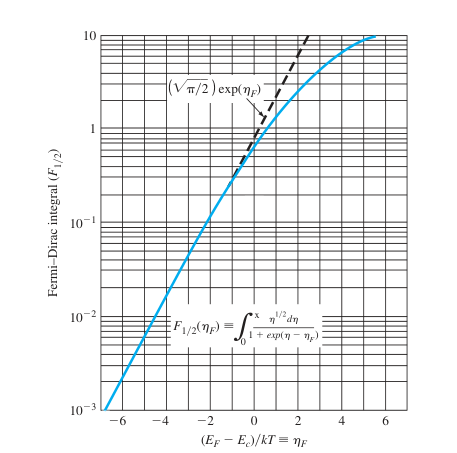
\includegraphics[width=0.8\linewidth]{feimi.png}
    \caption{费米统计与经典统计比较}
    \label{fig:feimi-classical}
\end{figure}
我们将$E_F$与$E_c$的相对位置作为区分简并与非简并的标准:
\begin{equation}
\left\{
\begin{aligned}
    &E_c-E_F>2k_0T \quad\text{非简并}\\
    &0<E_c-E_F\leq 2k_0T \quad\text{弱简并}\\
    &E_c-E_F\leq 0 \quad \text{简并}
\end{aligned}
\right.
\end{equation}





\chapter{半导体的导电性}

\section{载流子的漂移运动和迁移率}

\subsection{欧姆定律}

电阻为$R$的导体两端施加电压$V$,电流为
\begin{equation}
    I=\frac{V}{R}\label{eq:chap-4-ohms-law}
\end{equation}
电阻$R$与导体的长度$l$成正比,与截面积$s$成反比:
\begin{equation}
    R=\rho\frac{l}{s}\label{eq:chap-4-resistance-equation}
\end{equation}
$\rho$为导体的\textbf{电阻率},国际单位$[\rho]=\Omega\cdot\mathrm{m}$,常用单位为$\Omega\cdot\mathrm{cm}$。电阻率的倒数为电导率$\sigma$:
\begin{equation}
    \sigma=\frac{1}{\rho}\label{eq:chap-4-sigma-rho-relation}
\end{equation}
单位为$\mathrm{S}/\mathrm{m}$或$\mathrm{S}/\mathrm{cm}$。

\textbf{电流密度}$J$是通过垂直于电流方向的单位面积截面的电流:
\begin{equation}
    \bm J=\frac{\Delta \bm I}{\Delta s}
\end{equation}
$\bm J$是一个矢量,单位为$\mathrm{A/m^2}$或$\mathrm{A/cm^2}$

一段长$l$,截面$s$,电阻率$\rho$的均匀导体,两端加电压$V$,导体内部电场$\mathscr{E}$大小
\begin{equation}
    \mathscr{E}=\frac{V}{l}\label{eq:chap-4-electrical-field-strength}
\end{equation}
对均匀导体,电流密度
\begin{equation}
    \bm J=\frac{\bm I}{s}\label{eq:chap-4-uniform-conductor-I-density}
\end{equation}
将\autoref{eq:chap-4-electrical-field-strength},\autoref{eq:chap-4-uniform-conductor-I-density}和\autoref{eq:chap-4-resistance-equation}代入\autoref{eq:chap-4-ohms-law},得:
\begin{equation}
    sJ=\frac{\mathscr{E}l}{\D \rho\frac{l}{s}}
\end{equation}
化简得:
\begin{equation}
    J=\sigma\mathscr{E}\label{eq:chap-4-ohms-law-differential-form}
\end{equation}
上式即\textbf{欧姆定律微分形式}。

\subsection{漂移速度和迁移率}

外加电压下,导体电子受电场力作用,沿电场反方向作定向运动形成电流。这种定向运动称为\textbf{漂移运动},定向运动的速度称为\textbf{漂移速度}。用$\Bar{v}_d$表示漂移速度。

导体的任一截面A,设$n$为电子浓度,则单位时间通过的电子数
\begin{equation*}
    nq\Bar{v}_d\mathrm{d}ts
\end{equation*}
则电流为
\begin{equation}
    I=-\frac{nq\Bar{v}_d\mathrm{d}ts}{\mathrm{d}t}=-nq\Bar{v}_ds
\end{equation}
电流密度为
\begin{equation}
    J=\frac{I}{s}=-nq\Bar{v}_d
\end{equation}
恒定电场下,漂移速度与电场强度成正比:
\begin{equation}
    \Bar{v}_d=\mu\mathscr{E}
\end{equation}
$\mu$为电子的\textbf{迁移率},表示单位电场下电子平均漂移速度,单位$\mathrm{m^2/(V\cdot s)}$或$\mathrm{cm^2/(V\cdot s)}$。$\mu$习惯上只取正值:
\begin{equation}
    \mu=\left|\frac{\Bar{v}_d}{\mathscr{E}}\right|
\end{equation}
代入电流密度:
\begin{equation}
    J=nq\mu\mathscr{E}
\end{equation}
比较微分形式欧姆定律\autoref{eq:chap-4-ohms-law-differential-form},得到电导率:
\begin{equation}
    \sigma=nq\mu
\end{equation}
上式即电导率和迁移率的关系。

\subsection{半导体电导率和迁移率}

半导体中同时存在着电子和空穴,记$J_n$为电子电流密度,$J_p$为空穴电流密度,$n,\ p$分别为电子和空穴浓度,则总电流密度:
\begin{equation}
    J=J_n+J_p=\left(nq\mu_n+pq\mu_p\right)\mathscr{E}
\end{equation}
电导率为
\begin{equation}
    \sigma=nq\mu_n+pq\mu_p
\end{equation}
若两种载流子浓度悬殊,迁移率差别不大,则电导率主要取决于多数载流子:
\begin{enumerate}
    \item 对n型半导体,$n\gg p$,空穴对电流的贡献可以忽略,电导率为:
    \begin{equation}
        \sigma=nq\mu_n
    \end{equation}
    \item 对p型半导体,$p\gg n$,电导率为:
    \begin{equation}
        \sigma=pq\mu_p
    \end{equation}
\end{enumerate}
对于本征半导体,有$n=p=n_i$,电导率为
\begin{equation}
    \sigma_i=n_iq(\mu_n+\mu_p)
\end{equation}

\section{载流子的散射}

半导体内的载流子不断进行着\textbf{热运动}。热运动的载流子与晶格原子或电离杂质离子发生碰撞,其速度大小和方向会发生改变,即遭到\textbf{散射}。载流子在两次散射之间自由运动的平均路程称为\textbf{平均自由程},平均时间称为\textbf{平均自由时间}。

\section{迁移率与杂质浓度和温度的关系}

\subsection{平均自由时间与散射概率的关系}

记载流子的平均自由时间为$\tau$。设$0$时刻有$N_0$个电子以速度$v$沿某方向运动,$N(t)$为$t$时刻未散射的电子数。电子受到散射的概率为$P$,$\Delta t$时间内被散射电子数为:
\begin{equation*}
    N(t)P\Delta t
\end{equation*}
故$t$时刻未散射电子数$N(t)$比$t+\Delta t$时刻未散射电子数$N(t+\Delta t)$多$N(t)P\Delta t$:
\begin{equation}
    N(t)-N(t+\Delta t)=N(t)P\Delta t
\end{equation}
当$\Delta t\rightarrow \mathrm{d}t$时:
\begin{equation}
    \frac{\mathrm{d}N}{\mathrm{d}t}=\lim_{\Delta t\rightarrow 0}\frac{N(t)-N(t+\Delta t)}{\Delta t}=-PN(t)
\end{equation}
解这个微分方程,得:
\begin{equation}
    N(t)=N_0\mathrm{e}^{-Pt}
\end{equation}
故$t$到$t+\mathrm{d}t$时刻内被散射的电子数为:
\begin{equation*}
    N_0P\mathrm{e}^{-Pt}\mathrm{d}t
\end{equation*}
在$t$到$t+\mathrm{d}t$时刻内散射的电子的自由时间均为$t$,这些电子自由时间的总和为$N_0P\mathrm{e}^{-Pt}t\mathrm{d}t$。将它为全部时间积分再除以$N_0$即平均自由时间。故平均自由时间有:
\begin{equation}
    \tau=\frac{1}{N_0}\int_0^\infty N_0P\mathrm{e}^{-Pt}t\mathrm{d}t=\int_0^\infty P\mathrm{e}^{-Pt}t\mathrm{d}t=\frac{1}{P}
\end{equation}
即平均自由时间等于散射概率的倒数。

\subsection{电导率、迁移率和平均自由时间的关系}

电子在$0$时刻受到散射后沿$x$方向速度为$v_{x0}$,经$t$时刻再受到散射,此时速度为:
\begin{equation}
    v_x=v_{x0}+at=v_{x0}-\frac{q}{m_n^*}\mathscr{E}t
\end{equation}
故按上节的分析,$N_0$个电子的平均漂移速度$\Bar{v}_x$为:
\begin{align}
    \Bar{v}_x&=\Bar{v}_{x0}-\frac{1}{N_0}\int_0^\infty\frac{q}{m_n^*}\mathscr{E}tN_0P\mathrm{e}^{-Pt}\mathrm{d}t\\
    &=\Bar{v}_{x0}-\int_0^\infty\frac{q}{m_n^*}\mathscr{E}tP\mathrm{e}^{-Pt}\mathrm{d}t
\end{align}
由于$0$时刻速度$\bm v_0$方向随机,故$\bm v_0$在$x$方向上的平均值$\Bar{v}_{x0}=0$。所以:
\begin{equation}
    \Bar{v}_x=-\int_0^\infty\frac{q}{m_n^*}\mathscr{E}tP\mathrm{e}^{-Pt}\mathrm{d}t=-\frac{q\mathscr{E}}{m_n^*}\tau_n
\end{equation}
$\tau_n$为电子平均自由时间。

根据迁移率定义:
\begin{equation}
    \mu=\frac{\left|\Bar{v}_x\right|}{\mathscr{E}}
\end{equation}
得电子迁移率:
\begin{equation}
    \mu_n=\frac{q\tau_n}{m_n^*}
\end{equation}
同理,空穴迁移率:
\begin{equation}
    \mu_p=\frac{q\tau_p}{m_p^*}
\end{equation}
n型材料的电导率:
\begin{equation}
    \sigma_n=nq\mu_n=\frac{nq^2\tau_n}{m_n^*}
\end{equation}
p型材料电导率:
\begin{equation}
    \sigma_p=pq\mu_p=\frac{pq^2\tau_p}{m_p^*}
\end{equation}
混合型材料电导率:
\begin{equation}
    \sigma=nq\mu_n+pq\mu_p=\frac{nq^2\tau_n}{m_n^*}+\frac{pq^2\tau_p}{m_p^*}
\end{equation}

\subsection{电导有效质量}

对于等能面为旋转椭球面的多极值半导体,其晶体沿不同方向有效质量不同。

以Si为例,Si的导带等能面如\autoref{fig:homo-energy-phase}所示。椭圆长轴沿$<1\ 0\ 0>$方向。横向有效质量为$m_t$,纵向有效质量为$m_l$。取$x$轴,$y$轴,$z$轴分别沿$[1\ 0\ 0],\ [0\ 1\ 0],\ [0\ 0\ 1]$方向。设电场强度$\mathscr{E}$\vspace{1ex}
沿$x$轴方向,则电子沿$[1\ 0\ 0]$方向的迁移率$\mu_1=\D \frac{q\tau_n}{m_l}$,其他方向电子迁移率为$\mu_2=\mu_3=\D \frac{q\tau_n}{m_t}$。\vspace{1ex}
设电子浓度为$n$,平均每个能谷单位体积中有$\D \frac{n}{6}$个电子,则电流密度$J_x$为:
\begin{equation}
    J_x=\frac{1}{3}nq(\mu_1+\mu_2+\mu_3)\mathscr{E}
\end{equation}
令:
\begin{equation}
    J_x=nq\mu_c\mathscr{E}
\end{equation}
$\mu_c$为\textbf{电导迁移率}。比较上两式,得:
\begin{equation}
    \mu_c=\frac{1}{3}(\mu_1+\mu_2+\mu_3)
\end{equation}
$\mu_c$可以写成
\begin{equation}
    \mu_c=\frac{q\tau_n}{m_c}
\end{equation}
即:
\begin{align}
    \frac{q\tau_n}{m_c}&=\frac{1}{3}(\mu_1+\mu_2+\mu_3)\\
    &=\frac{1}{3}\left(\frac{q\tau_n}{m_l}+\frac{2q\tau_n}{m_t}\right)
\end{align}
故有:
\begin{equation}
    \frac{1}{m_c}=\frac{1}{3}\left(\frac{1}{m_l}+\frac{2}{m_t}\right)
\end{equation}
$m_c$即为\textbf{电导有效质量}。

\subsection{电阻率}

由\autoref{eq:chap-4-sigma-rho-relation}可知,电阻率是电导率的倒数:
\begin{equation}
    \rho=\frac{1}{\sigma}=\frac{1}{nq\mu_n+pq\mu_p}
\end{equation}
对于n型半导体:
\begin{equation}
    \rho_n=\frac{1}{nq\mu_n}
\end{equation}
p型半导体:
\begin{equation}
    \rho_p=\frac{1}{pq\mu_p}
\end{equation}
本征半导体:
\begin{equation}
    \rho_i=\frac{1}{n_iq(\mu_n+\mu_p)}
\end{equation}
















\chapter{非平衡载流子}

\section{非平衡载流子的注入和复合}

处于热平衡下的载流子浓度称为\textbf{平衡载流子浓度}。一般用$n_0$和$p_0$分别表示平衡电子浓度和空穴浓度。非简并条件下,其乘积满足关系:
\begin{equation}
    n_0p_0=N_vN_c\exp{\left(-\frac{E_g}{k_0T}\right)}=n_i^2
\end{equation}

对半导体施加外界作用,破坏热平衡条件,使半导体处于与热平衡偏离的状态,称为\textbf{非平衡状态}。处于非平衡状态的半导体,其载流子浓度浓度不再为$n_0$和$p_0$,而会多出一部分。比平衡状态多出的载流子称为\textbf{非平衡载流子}或\textbf{过剩载流子}。

一定温度下,n型半导体中,$n_0\gg p_0$,用适当波长的光照射半导体,且光子能量大于半导体的禁带宽度,则光子可以将价带电子激发到导带上,形成电子-空穴对,导带比平衡时多出$\Delta n$的电子,即\textbf{非平衡电子},称为\textbf{非平衡多数载流子(多子)};价带多出$\Delta p$的空穴,即\textbf{非平衡空穴},称为\textbf{非平衡少数载流子(少子)}。这种通过光照产生非平衡载流子的方法,称为非平衡载流子的\textbf{光注入}。光注入时有:
\begin{equation}
    \Delta n=\Delta p
\end{equation}

一般情况下,注入的非平衡载流子浓度比平衡时的多数载流子浓度小得多。对上述情况,有:
\begin{equation}
    \Delta n\ll n_0,\quad \Delta p\ll n_0
\end{equation}
满足此条件的注入称为\textbf{小注入}。在小注入条件下,非平衡少子的浓度也可以比平衡少子的浓度大得多,如上例中有$\Delta p\gg p_0$。非平衡少子常常会起决定性作用。通常所说的非平衡载流子都指非平衡少子。

光注入导致半导体的电导率增大。附加电导率为:
\begin{equation}
    \Delta \sigma=\Delta nq\mu_n+\Delta pq\mu_p=\Delta pq(\mu_n+\mu_p)
\end{equation}

设半导体平衡电导率为$\sigma_0$,光照引起附加电导率$\Delta \sigma$,小注入条件下$\sigma_0+\Delta \sigma\approx\sigma_0$,电阻率改变:
\begin{equation}
    \Delta\rho=\frac{1}{\sigma}-\frac{1}{\sigma_0}=\frac{1}{\sigma_0+\Delta\sigma}-\frac{1}{\sigma_0}=-\frac{\Delta\sigma}{(\sigma_0+\Delta\sigma)\sigma_0}\approx-\frac{\Delta\sigma}{\sigma_0^2}
\end{equation}
半导体电阻改变:
\begin{equation}
    \Delta r=\Delta\rho\frac{l}{s}\approx-\frac{l}{s\sigma_0^2}\Delta\sigma
\end{equation}
$l,\ s$为半导体的长度和截面积。因此$\Delta r\propto \Delta \sigma$。半导体通电时,由于电势差$\Delta V=I\Delta r$,故$\Delta V\propto\Delta\sigma$,因此$\Delta V\propto\Delta p$:
\begin{equation}
    \Delta V=-\frac{l}{s\sigma^2}Iq(\mu_n+\mu_p)\Delta p
\end{equation}

\section{非平衡载流子的寿命}

小注入时,$\Delta V$的变化反映了$\Delta p$的变化。光照停止后,$\Delta p$随时间按指数减小。非平衡载流子的平均生存时间称为载流子的\textbf{寿命},用$\tau$表示(上章有个叫平均自由时间的物理量也记成$\tau$ 
\includegraphics[width=4em, align=c]{idiot.jpg})。由于非平衡少子相比多子更占主导地位,因此非平衡载流子的寿命常称为\textbf{少子的寿命}。显然$\D \frac{1}{\tau}$是单位时间内非平衡载流子的复合概率。\vspace{1ex}
通常将单位时间单位体积内净复合消失的电子-空穴对数称为非平衡载流子的\textbf{复合率}。显然,$\D \frac{\Delta p}{\tau}$就是复合率。

一束光在一块n型半导体内均匀产生非平衡载流子$\Delta n$和$\Delta p$。$t=0$时光照停止,\vspace{1ex}
$\Delta p$会随时间变化,单位时间内浓度减小$\D -\frac{\mathrm{d}\Delta p(t)}{\mathrm{d}t}$,减小是由电子-空穴对的复合引起的,应当等于非平衡载流子的复合率:
\begin{equation}
    \frac{\mathrm{d}\Delta p(t)}{\mathrm{d}t}=-\frac{\Delta p}{\tau}
\end{equation}
寿命$\tau$在小注入条件下是个恒量,与$\Delta p(t)$无关。解这个微分方程:
\begin{equation}
    \Delta p(t)=C\mathrm{e}^{-\frac{t}{\tau}}
\end{equation}
设$t=0$时刻停止光照时少子浓度$\Delta p(0)=\Delta p_0$,作为边界条件代入微分方程,解得系数为$C=\Delta p_0$,故:
\begin{equation}
    \Delta p(t)=\Delta p_0\mathrm{e}^{-\frac{t}{\tau}}
\end{equation}
即非平衡载流子浓度随时间按指数衰减。

\section{准费米能级}

热平衡下的半导体中电子和空穴具有统一的费米能级。非简并条件下:
\begin{equation}
    n_0=N_c\exp{\left(-\frac{E_c-E_F}{k_0T}\right)},\quad p_0=N_v\exp{\left(-\frac{E_F-E_v}{k_0T}\right)}\label{eq:chap-5-equilibrium-distribute}
\end{equation}
外界影响下破坏了热平衡,非平衡态的半导体不再具有统一的费米能级。我们认为价带和导带中的电子与空穴各自处于平衡状态,但价带与导带之间不处于平衡态。因此可以分别引入\textbf{导带费米能级}和\textbf{价带费米能级},均为\textbf{局部费米能级},称为\textbf{准费米能级}。导带费米能级也称为\textbf{电子准费米能级},用$E_{Fn}$表示,价带准费米能级也称为\textbf{空穴准费米能级},用$E_{Fp}$表示。

非平衡下的载流子浓度可以用与平衡载流子浓度类似公式表达:
\begin{equation}
    n=N_c\exp{\left(-\frac{E_c-E_{Fn}}{k_0T}\right)},\quad p=N_v\exp{\left(-\frac{E_{Fp}-E_v}{k_0T}\right)}
\end{equation}
上式适用的条件与平衡态载流子相同,即$E_{Fn}$和$E_{Fp}$不能进入导带或价带。参考\autoref{eq:chap-5-equilibrium-distribute},可以推导出$n$与$n_0$,$p$与$p_0$的关系:
\begin{align}
&
\begin{aligned}
    n&=N_c\exp{\left(-\frac{E_c-E_{Fn}}{k_0T}\right)}\\
    &=N_c\exp{\left(-\frac{E_c-E_{F}}{k_0T}\right)}\exp{\left(\frac{E_{Fn}-E_F}{k_0T}\right)}\\
    &=n_0\exp{\left(\frac{E_{Fn}-E_F}{k_0T}\right)}
\end{aligned}
\\
&
\begin{aligned}
    p&=N_v\exp{\left(-\frac{E_{Fp}-E_v}{k_0T}\right)}\\
    &=N_v\exp{\left(-\frac{E_{F}-E_v}{k_0T}\right)}\exp{\left(\frac{E_F-E_{Fp}}{k_0T}\right)}\\
    &=p_0\exp{\left(\frac{E_F-E_{Fp}}{k_0T}\right)}
\end{aligned}
\end{align}
由
\begin{equation}
    n_0=n_i\exp{\left(-\frac{E_i-E_F}{k_0T}\right)},\quad p_0=n_i\exp{\left(\frac{E_i-E_F}{k_0T}\right)}
\end{equation}
进一步推导:
\begin{align}
&
    \begin{aligned}
        n&=n_0\exp{\left(\frac{E_{Fn}-E_F}{k_0T}\right)}\\
        &=n_i\exp{\left(-\frac{E_i-E_F}{k_0T}\right)}\exp{\left(\frac{E_{Fn}-E_F}{k_0T}\right)}\\
        &=n_i\exp{\left(\frac{E_{Fn}-E_i}{k_0T}\right)}
    \end{aligned}
    \\
&
    \begin{aligned}
        p&=p_0\exp{\left(\frac{E_F-E_{Fp}}{k_0T}\right)}\\
        &=n_i\exp{\left(\frac{E_i-E_F}{k_0T}\right)}\exp{\left(\frac{E_F-E_{Fp}}{k_0T}\right)}\\
        &=n_i\exp{\left(\frac{E_i-E_{Fp}}{k_0T}\right)}
    \end{aligned}
\end{align}
电子与空穴浓度的乘积:
\begin{equation}
    np=n_0p_0\exp{\left(\frac{E_{Fn}-E_{Fp}}{k_0T}\right)}
\end{equation}

\section{复合理论}

\subsection{载流子复合的分类}

半导体\textbf{复合}的过程即半导体\textbf{由非平衡态向平衡态过渡}的过程。半导体的复合过程大致可分为:
\begin{enumerate}
    \item 直接复合:电子在导带与价带间直接跃迁,实现电子与空穴的复合。
    \item 间接复合:电子与空穴通过禁带能级复合。简介复合按照发生位置可以分为\textbf{体内复合}和\textbf{表面复合}。
\end{enumerate}
载流子复合时会放出多余能量,放出能量的方法有:
\begin{enumerate}
    \item 发射光子:伴随复合,伴有发光现象,称为\textbf{发光复合}或\textbf{辐射复合}。
    \item 发射声子:载流子将多余能量传递给晶格,加强晶格振动。
    \item 能量给予其他载流子,增大动能,称为\textbf{俄歇(Auger)复合}。
\end{enumerate}

\subsection{直接复合}

半导体中同时存在着载流子的\textbf{产生}和和\textbf{复合}两个过程。单位时间内产生的电子-空穴对数称为\textbf{产生率},记为$G$,复合的电子-空穴对数称为\textbf{复合率},记为$R$。

$n,\ p$分别为电子和空穴浓度。单位体积,单位时间里,每个电子都有概率和空穴复合,复合概率与空穴浓度成正比,即每个电子复合的概率为$rp$,$r$是比例系数。每个电子复合概率再乘以电子浓度就是全部电子的复合率,即:
\begin{equation}
    R=rnp
\end{equation}
比例系数$r$称为\textbf{电子-空穴复合概率},它代表着所有电子和空穴复合概率的平均值。

载流子受激发的概率不受载流子浓度的影响,产生率在所有非简并情况下是相同的,即$G$仅与温度有关,和$n,\ p$无关。

热平衡时,产生率等于复合率:$P=G$,此时$n=n_0,\ p=p_0$,因此得到$G$与$r$的关系:
\begin{equation}
    G=P=rn_0p_0=rn_i^2
\end{equation}
复合率减产生率即非平衡载流子的净复合率,得到净复合率$U_d$为:
\begin{equation}
    U_d=R-G=rnp-rn_i^2=r(np-n_i^2)
\end{equation}
代入关系$n=n_0+\Delta n,\ p=p_0+\Delta p,\ \Delta n=\Delta p$,得:
\begin{align}
    U_d&=r[(n_0+\Delta n)(p_0+\Delta p)-n_0p_0]\notag\\
    &=r(n_0\Delta p+p_0\Delta p+\Delta p^2)\notag\\
    &=r(n_0+p_0)\Delta p+r\Delta p^2
\end{align}
由于净复合率和载流子寿命存在关系:
\begin{equation}
    U_d=\frac{\Delta p}{\tau}
\end{equation}
得载流子寿命:
\begin{equation}
    \tau=\frac{\Delta p}{U_d}=\frac{1}{r[(n_0+p_0)+\Delta p]}\label{eq:chap-5-direct-recombination-lifetime}
\end{equation}
可见寿命$\tau$不仅与平衡载流子浓度有关,也与非平衡载流子浓度有关。

在小注入条件下,$\Delta p\ll (n_0+p_0)$,\autoref{eq:chap-5-direct-recombination-lifetime}近似为:
\begin{equation}
    \tau\approx\frac{1}{r(n_0+p_0)}
\end{equation}
对n型材料,$n_0\gg p_0$,上式近似有
\begin{equation}
    \tau\approx\frac{1}{rn_0}
\end{equation}
寿命与非平衡载流子无关,与多数载流子成反比。

当$\Delta p\gg n_0+p_0$时,\autoref{eq:chap-5-direct-recombination-lifetime}近似有:
\begin{equation}
    \tau\approx\frac{1}{r\Delta p}
\end{equation}
此时寿命与非平衡载流子成反比。

\subsection{间接复合}

半导体中的杂质和缺陷会促进非平衡载流子的复合过程,这些促进复合的杂质和缺陷称为\textbf{复合中心}。间接复合即非平衡载流子通过复合中心的复合。

记复合中心能级$E_t$,如\autoref{fig:indirect-recombination-process},能级$E_t$上的间接复合具有四个过程:
\begin{enumerate}[(1)]
    \item 俘获电子:复合中心能级$E_t$从导带俘获电子。
    \item 发射电子:复合中心能级$E_t$上的电子被激发到导带。
    \item 俘获空穴:电子由复合中心能级$E_t$落入价带,与空穴复合,可以看成复合中心能级$E_t$从价带俘获一个电子。
    \item 发射空穴:价带电子激发到复合中心能级$E_t$,可以看出复合中心能级$E_t$向价带发射一个空穴。
\end{enumerate}

\begin{figure}[ht]
    \centering
\tikzset{every picture/.style={line width=0.75pt}} %set default line width to 0.75pt        

\begin{tikzpicture}[x=0.75pt,y=0.75pt,yscale=-1,xscale=1]
%uncomment if require: \path (0,300); %set diagram left start at 0, and has height of 300

%Straight Lines [id:da20064609469527683] 
\draw    (120.67,31.08) -- (137.17,31.09) -- (253.17,31.1) ;
%Straight Lines [id:da19330925404980026] 
\draw  [dash pattern={on 4.5pt off 4.5pt}]  (120.17,77.5) -- (252.67,77.5) ;
%Straight Lines [id:da5528060898844296] 
\draw    (120.17,125) -- (252.67,125) ;
%Shape: Circle [id:dp32843318610089023] 
\draw  [fill={rgb, 255:red, 0; green, 0; blue, 0 }  ,fill opacity=1 ] (134.63,31.09) .. controls (134.63,32.49) and (135.76,33.63) .. (137.17,33.63) .. controls (138.57,33.63) and (139.71,32.49) .. (139.71,31.09) .. controls (139.71,29.68) and (138.57,28.54) .. (137.17,28.54) .. controls (135.76,28.54) and (134.63,29.68) .. (134.63,31.09) -- cycle ;
%Straight Lines [id:da48904866335535435] 
\draw    (137.17,31.09) -- (137.17,74.58) ;
\draw [shift={(137.17,77.58)}, rotate = 270] [fill={rgb, 255:red, 0; green, 0; blue, 0 }  ][line width=0.08]  [draw opacity=0] (10.72,-5.15) -- (0,0) -- (10.72,5.15) -- (7.12,0) -- cycle    ;
%Straight Lines [id:da7345813081514647] 
\draw    (160.67,33.09) -- (160.67,76.58) ;
\draw [shift={(160.67,30.09)}, rotate = 90] [fill={rgb, 255:red, 0; green, 0; blue, 0 }  ][line width=0.08]  [draw opacity=0] (10.72,-5.15) -- (0,0) -- (10.72,5.15) -- (7.12,0) -- cycle    ;
%Shape: Circle [id:dp42146991706121617] 
\draw  [fill={rgb, 255:red, 0; green, 0; blue, 0 }  ,fill opacity=1 ] (158.12,76.58) .. controls (158.12,77.99) and (159.26,79.13) .. (160.67,79.13) .. controls (162.07,79.13) and (163.21,77.99) .. (163.21,76.58) .. controls (163.21,75.18) and (162.07,74.04) .. (160.67,74.04) .. controls (159.26,74.04) and (158.12,75.18) .. (158.12,76.58) -- cycle ;
%Straight Lines [id:da21853964923058133] 
\draw    (195.17,77.59) -- (195.17,121.08) ;
\draw [shift={(195.17,124.08)}, rotate = 270] [fill={rgb, 255:red, 0; green, 0; blue, 0 }  ][line width=0.08]  [draw opacity=0] (10.72,-5.15) -- (0,0) -- (10.72,5.15) -- (7.12,0) -- cycle    ;
%Shape: Circle [id:dp8914894742891817] 
\draw  [fill={rgb, 255:red, 0; green, 0; blue, 0 }  ,fill opacity=1 ] (192.63,77.59) .. controls (192.63,78.99) and (193.76,80.13) .. (195.17,80.13) .. controls (196.57,80.13) and (197.71,78.99) .. (197.71,77.59) .. controls (197.71,76.18) and (196.57,75.04) .. (195.17,75.04) .. controls (193.76,75.04) and (192.63,76.18) .. (192.63,77.59) -- cycle ;
%Straight Lines [id:da2456794806958813] 
\draw    (232.67,80.59) -- (232.67,124.08) ;
\draw [shift={(232.67,77.59)}, rotate = 90] [fill={rgb, 255:red, 0; green, 0; blue, 0 }  ][line width=0.08]  [draw opacity=0] (10.72,-5.15) -- (0,0) -- (10.72,5.15) -- (7.12,0) -- cycle    ;
%Shape: Circle [id:dp5273521015953397] 
\draw  [fill={rgb, 255:red, 0; green, 0; blue, 0 }  ,fill opacity=1 ] (230.12,124.08) .. controls (230.12,125.49) and (231.26,126.63) .. (232.67,126.63) .. controls (234.07,126.63) and (235.21,125.49) .. (235.21,124.08) .. controls (235.21,122.68) and (234.07,121.54) .. (232.67,121.54) .. controls (231.26,121.54) and (230.12,122.68) .. (230.12,124.08) -- cycle ;

% Text Node
\draw (115.67,43) node [anchor=north west][inner sep=0.75pt]   [align=left] {(1)};
% Text Node
\draw (162,43) node [anchor=north west][inner sep=0.75pt]   [align=left] {(2)};
% Text Node
\draw (173.67,93) node [anchor=north west][inner sep=0.75pt]   [align=left] {(3)};
% Text Node
\draw (233.17,93) node [anchor=north west][inner sep=0.75pt]   [align=left] {(4)};
% Text Node
\draw (254.67,116.9) node [anchor=north west][inner sep=0.75pt]    {$E_{v}$};
% Text Node
\draw (254.17,23.9) node [anchor=north west][inner sep=0.75pt]    {$E_{c}$};
% Text Node
\draw (254.67,69.4) node [anchor=north west][inner sep=0.75pt]    {$E_{t}$};
\end{tikzpicture}
    \caption{复合中心能级$E_t$的四个间接复合过程}
    \label{fig:indirect-recombination-process}
\end{figure}

$n$和$p$分别为导带电子和价带空穴浓度,设复合中心浓度为$N_t$,复合中心能级上的电子浓度为$n_t$,则未被电子占据的复合中心浓度为$N_t-n_t$。

(1) 过程中,我们把单位体积、单位时间内内复合中心俘获的电子数称为\textbf{电子俘获率}。电子俘获率与导带电子浓度$n$和未被占据的复合中心浓度$(N_t-n_t)$成正比:
\begin{equation}
    \text{电子俘获率}=r_nn(N_t-n_t)\label{eq:chap-5-indirect-recombination-electron-capture-rate}
\end{equation}
比例系数$r_n$是\textbf{电子俘获系数},反映了复合中心平均俘获电子能力的大小。

(2) 过程是 (1) 过程的逆过程。我们用电子产生率表示单位时间、单位体积向导带发射的电子数。只有已被占据的复合中心才能向导带发射电子,导带近似认为是空的,因此电子产生率与$n_t$成正比,和$n$无关:
\begin{equation}
    \text{电子产生率}=s_-n_t
\end{equation}
$s_-$称为\textbf{电子激发概率},仅与温度有关。

平衡时,(1) 过程和 (2) 过程相互抵消,电子产生率等于电子俘获率:
\begin{equation}
    r_nn_0(N_t-n_{t0})=s_-n_{t0}\label{eq:chap-5-equilibrium-indirect-recombination-electron-equation}
\end{equation}
$n_0$和$n_{t0}$分别为平衡时导带和复合中心能级上的电子浓度。计算$n_{t0}$时,我们忽略分布函数中的简并因子:
\begin{equation}
    n_{t0}=N_tf(E_t)=N_t\frac{1}{\D 1+\exp{\left(\frac{E_t-E_F}{k_0T}\right)}}
\end{equation}
非简并条件下:
\begin{equation}
    n_0=N_c\exp{\left(\frac{E_F-E_c}{k_0T}\right)}
\end{equation}
将$n_0$和$n_{t0}$表达式代入\autoref{eq:chap-5-equilibrium-indirect-recombination-electron-equation}:
\begin{align}
    s_-N_t\frac{1}{\D 1+\exp{\left(\frac{E_t-E_F}{k_0T}\right)}}&=r_nN_c\exp{\left(\frac{E_F-E_c}{k_0T}\right)}N_t\left[1-\left(\frac{1}{\D 1+\exp{\left(\frac{E_t-E_F}{k_0T}\right)}}\right)\right]\notag\\
    \Longrightarrow s_-&=r_nN_c\exp{\left(\frac{E_F-E_c}{k_0T}\right)}\exp{\left(\frac{E_t-E_F}{k_0T}\right)}\notag\\
    \Longrightarrow s_-&=r_nN_c\exp{\left(\frac{E_t-E_c}{k_0T}\right)}
\end{align}
记:
\begin{equation}
    n_1=N_c\exp{\left(\frac{E_t-E_c}{k_0T}\right)}
\end{equation}
$n_1$等于费米能级与复合中心能级重合时导带电子平均浓度。代入:
\begin{equation}
    s_-=r_nN_c\exp{\left(\frac{E_t-E_c}{k_0T}\right)}=r_nn_1
\end{equation}
将上式代入电子产生率中:
\begin{equation}
    \text{电子产生率}=r_nn_1n_t\label{eq:chap-5-indirect-recombination-electron-generation-rate}
\end{equation}

(3) 过程中,空穴俘获率与$n_t$和$p$成正比:
\begin{equation}
    \text{空穴俘获率}=r_ppn_t\label{eq:chap-5-indirect-recombination-hole-capture-rate}
\end{equation}
$r_p$称为\textbf{空穴俘获系数},反映复合中心平均俘获空穴的能力.

(4) 过程是 (3) 的逆过程类似上文讨论,有:
\begin{equation}
    \text{空穴产生率}=s_+(N_t-n_t)
\end{equation}
$s_+$为\textbf{空穴激发概率}。

平衡时,(3) 和 (4) 过程相互抵消:
\begin{equation}
    s_+(N_t-n_{t0})=r_pp_0n_{t0}
\end{equation}
代入平衡时$p_0$和$n_{t0}$值,得:
\begin{equation}
    s_+=r_pp_1
\end{equation}
其中
\begin{equation}
    p_1=N_v\exp{\left(-\frac{E_t-E_v}{k_0T}\right)}
\end{equation}
$p_1$等于费米能级和复合中心能级重合时价带的平衡空穴浓度。

将$s_+$表达式代入空穴产生率,得:
\begin{equation}
    \text{空穴产生率}=r_pp_1(N_t-n_t)\label{eq:chap-5-indirect-recombination-hole-generation-rate}
\end{equation}
在稳定情况下,(1) 到 (4) 过程满足复合中心上电子数不变,即$n_t$为常数。由于 (1)  (4)两个过程造成复合中心上电子累积,(2) (3) 两个过程造成复合中心上电子的减少,为保持$n_t$不变,满足:
\begin{equation}
    \text{(1)}+\text{(4)}=\text{(2)}+\text{(3)}
\end{equation}
代入\autoref{eq:chap-5-indirect-recombination-electron-capture-rate}、\autoref{eq:chap-5-indirect-recombination-electron-generation-rate}、\autoref{eq:chap-5-indirect-recombination-hole-capture-rate}、\autoref{eq:chap-5-indirect-recombination-hole-generation-rate}:
\begin{equation}
    r_nn(N_t-n_t)+r_pp_1(N_t-n_t)=r_nn_1n_t+r_ppn_t\label{eq:chap-5-indirect-recombination-center-electron-conecntration-equation}
\end{equation}
求解$n_t$,得:
\begin{equation}
    n_t=N_t\frac{r_nn+r_pp_1}{r_n(n+n_1)+r_p(p+p_1)}\label{eq:chap-5-indirect-recombination-center-electron-conecntration}
\end{equation}

半导体的电子复合率为 $\text{(1)}-\text{(2)}$,空穴复合率为 $\text{(3)}-\text{(4)}$由于电子和空穴成对出现,二者应相等,等于半导体的净复合率$U_d$:
\begin{equation}
    U=\text{(1)}-\text{(2)}=\text{(3)}-\text{(4)}
\end{equation}
将\autoref{eq:chap-5-indirect-recombination-center-electron-conecntration-equation}代入上式:
\begin{equation}
    U=N_t\frac{r_nr_p\left(np-n_1p_1\right)}{r_n(n+n_1)+r_p(p+p_1)}\label{eq:chap-5-indirect-recombination-center-total-recombination-rate-1}
\end{equation}
由于:
\begin{equation}
    n_1=N_c\exp{\left(\frac{E_t-E_c}{k_0T}\right)},\quad p_1=N_v\exp{\left(-\frac{E_t-E_v}{k_0T}\right)}
\end{equation}
得到:
\begin{equation}
    n_1p_1=N_cN_v\exp{\left(\frac{E_v-E_c}{k_0T}\right)}=n_i^2
\end{equation}
代入\autoref{eq:chap-5-indirect-recombination-center-total-recombination-rate-1},得到非平衡载流子复合率:
\begin{equation}
    U=N_t\frac{r_nr_p\left(np-n_i^2\right)}{r_n(n+n_1)+r_p(p+p_1)}\label{eq:chap-5-indirect-recombination-center-charge-carrier-total-recombination-rate}
\end{equation}
上式即通过复合中心复合的净复合率一般公式。

热平衡条件下,$np=n_0p_0=n_i^2$,代入\autoref{eq:chap-5-indirect-recombination-center-charge-carrier-total-recombination-rate},显然有$U=0$。

对半导体注入非平衡载流子,有$np>n_i^2$,$U>0$。代入关系$n=n_0+\Delta n,\ p=p_0+\Delta p,\ \Delta n=\Delta p$:
\begin{equation}
    U=N_t\frac{r_nr_p\left(n_0\Delta p+p_0\Delta p+\Delta p^2\right)}{r_n\left(n_0+n_1+\Delta p\right)+r_p\left(p_0+p_1+\Delta p\right)}
\end{equation}
非平衡载流子的寿命为:
\begin{equation}
    \tau=\frac{\Delta p}{U}=\frac{r_n\left(n_0+n_1+\Delta p\right)+r_p\left(p_0+p_1+\Delta p\right)}{N_tr_nr_p(n_0+p_0+\Delta p)}
\end{equation}
寿命$\tau$和复合中心浓度$N_t$成反比。

在小注入条件下$\Delta p\ll (n_0+p_0)$,对于一般的复合中心,$r_n$和$r_p$相差不大,分子和分母上的$\Delta p$可以忽略:
\begin{equation}
    \tau=\frac{r_n(n_0+n_1)+r_p(p_0+p_1)}{N_tr_nr_p(n_0+p_0)}
\end{equation}
可见小注入条件下,寿命与非平衡载流子浓度无关。

对于n型半导体,假定复合中心能级$E_t$接近价带,并令$E_t$关于禁带中心对称的能级位置为$E_t'$,$E_F$比$E_t'$更接近$E_c$,此时称为\textbf{强n型区},满足$n_0\gg p_0,\ n_0\gg n_1,\ n_0\gg p_1$,寿命化为:
\begin{equation}
    \tau=\tau_p\approx\frac{1}{N_t\tau_p}\label{eq:chap-5-indirect-recombination-n-type-strong-n-lifetime}
\end{equation}
因此在重掺杂的n型半导体中,对寿命起决定性作用的是复合中心对少数载流子(空穴)的俘获系数$r_p$,与电子俘获系数$r_n$无关。

若$E_F$在$E_i$和$E_t'$之间,称为\textbf{高阻区}。此时$p_1\gg n_0,\ p_1\gg p_0,\ p_1\gg n_1$,同时$n_0\gg p_0$,寿命:
\begin{equation}
    \tau\approx\frac{p_1}{N_tr_n}\frac{1}{n_0}
\end{equation}
高阻区中的寿命与多子浓度成反比,即与电导率成反比。

对于p型材料,仍假定$E_t$接近价带,当$E_F$比$E_t$更接近$E_v$时,称为\textbf{强p型区},寿命为:
\begin{equation}
    \tau=\tau_n\approx\frac{1}{N_tr_n}\label{eq:chap-5-indirect-recombination-p-type-strong-p-lifetime}
\end{equation}
可见复合中心对少子的俘获决定寿命。对\textbf{高阻区},有:
\begin{equation}
    \tau\approx\frac{p_1}{N_tr_n}\frac{1}{p_0}
\end{equation}
\vspace{1ex}若复合中心更接近导带,则高阻区的寿命公式中$\D\frac{p_1}{r_n}$应当用$\D \frac{n_1}{r_p}$代替。

将强n区寿命\autoref{eq:chap-5-indirect-recombination-n-type-strong-n-lifetime}和强p区寿命\autoref{eq:chap-5-indirect-recombination-p-type-strong-p-lifetime}代入非平衡载流子复合率
\autoref{eq:chap-5-indirect-recombination-center-charge-carrier-total-recombination-rate},得:
\begin{align}
    U&=\frac{np-n_i^2}{\D \frac{1}{N_tr_p}(n+n_1)+\frac{1}{N_tr_n}(p+p_1)}\notag\\
    &=\frac{np-n_i^2}{\tau_p(n+n_1)+\tau_n(p+p_1)}
\end{align}
由于
\begin{equation}
    n_1=n_i\exp{\left(\frac{E_t-E_i}{k_0T}\right)},\quad p_1=n_i\exp{\left(\frac{E_i-E_t}{k_0T}\right)}
\end{equation}
代入:
\begin{equation}
    U=\frac{np-n_i^2}{\D \tau_p\left[n+n_i\exp{\left(\frac{E_t-E_i}{k_0T}\right)}\right]+\tau_n\left[p+n_i\exp{\left(\frac{E_i-E_t}{k_0T}\right)}\right]}\label{eq:chap-5-indirect-recombination-center-charge-carrier-total-recombination-rate-Ei-Et}
\end{equation}
\vspace{1ex}假定$r=r_n=r_p$,则$\D \tau_n=\tau_p=\frac{1}{N_tr}$,化简,得:
\begin{align}
    U&=\frac{N_tr\left(np-n_i^2\right)}{\D n+p+n_i\left[\exp{\left(\frac{E_t-E_i}{k_0T}\right)}+\exp{\left(-\frac{E_t-E_i}{k_0T}\right)}\right]}\notag\\
    &=\frac{N_tr\left(np-n_i^2\right)}{\D n+p+2n_i\cosh{\left(\frac{E_t-E_i}{k_0T}\right)}}
\end{align}
\vspace{1ex}可以看出,$E_t\approx E_i$时,$\D\cosh{\left(\frac{E_t-E_i}{k_0T}\right)}\rightarrow \cosh{(0)}=1$极小,$U$趋于极大。如Cu,Fe,Au等杂质在Si中形成深能级,是有效的复合中心。远离禁带中央的浅能级不能起到有效的复合中心作用。

我们假设复活中心是具有一定半径的球体,其截面为$\sigma$。截面积越大,载流子运动中被复合中心俘获概率越大。因此可以用$\sigma$表示复合中心俘获载流子的本领,称为\textbf{俘获截面}。复合中心俘获电子和空穴的本领不同,因此分别用\textbf{电子俘获截面}$\sigma_+$和\textbf{空穴俘获截面}$\sigma_-$来表示。

载流子热运动速度$v_T$越大,它被复合中心俘获的概率也就越大。按照统计力学计算,得到$\D v_T=\sqrt{\frac{3k_0T}{m^*}}$。
若不区分电子和空穴有效质量,$300\ \mathrm{K}$时,有$v_T=10^7\ \mathrm{cm/s}$。\vspace{1ex}

俘获截面与俘获系数的关系有:
\begin{equation}
    r_n=\sigma_-v_T,\quad r_p=\sigma_+v_T
\end{equation}
利用此关系,可将\autoref{eq:chap-5-indirect-recombination-center-charge-carrier-total-recombination-rate-Ei-Et}重写为:
\begin{equation}
    U=\frac{\sigma_+\sigma_-v_TN_t(np-n_i^2)}{\D \sigma_-\left[n+n_i\exp{\left(\frac{E_t-E_i}{k_0T}\right)}\right]+\sigma_+\left[p+n_i\exp{\left(\frac{E_i-E_t}{k_0T}\right)}\right]}
\end{equation}
实验表明,Mn,Fe,Co,Au,Cu,Ni可以在Ge中形成复合中心;Au,Cu,Fe,Mn,In可以在Si中形成复合中心。

\subsection{表面复合}

少子寿命很大程度上受半导体样品的形状和表面状态影响。\textbf{表面复合}指在半导体表面发生的复合过程。表面的杂质和缺陷在禁带形成复合中心能级,因此表面复合仍是间接复合。

实际测得的寿命是体内复合和表面复合的综合结果。设这两种复合同时地单独平行发生,\vspace{1ex}
记体内复合寿命为$\tau_v$,
\vspace{1ex}则$\D \frac{1}{\tau_v}$就是体内复合概率。记表面复合寿命为$\tau_s$,则$\D \frac{1}{\tau_s}$就是表面复合概率。总概率为:
\begin{equation}
    \frac{1}{\tau}=\frac{1}{\tau_v}+\frac{1}{\tau_s}
\end{equation}
$\tau$称为\textbf{有效寿命}。

把单位时间内通过单位表面积复合的电子-空穴对数称为\textbf{表面复合率},记$U_s$。表面复合率$U_s$与表面处非平衡载流子浓度$\Delta p_s$成正比:
\begin{equation}
    U_s=s\Delta p_s
\end{equation}
比例系数$s$表示表面复合的强弱,量纲为速度,称为\textbf{表面复合速度}。

\section{陷阱效应}

能级上的电子通过载流子的俘获和产生过程和载流子保持平衡。对于非平衡态的载流子,这种平衡会受到破坏。电子增加,说明能级有收容非平衡载流子的作用;电子减少,说明能级有收容空穴的作用。杂质能级积累非平衡载流子的作用称为\textbf{陷阱效应}。所有的杂质能级都有陷阱效应,我们只考虑能够显著积累非平衡载流子的杂质能级。我们把具有显著陷阱效应的杂质能级称为\textbf{陷阱},相应的杂质和缺陷称为\textbf{陷阱中心}。

杂质能级上电子数如\autoref{eq:chap-5-indirect-recombination-center-electron-conecntration}。$n_t$与$\Delta n$和$\Delta p$有关,小注入条件下,杂质能级电子积累有:
\begin{equation}
    \Delta n_t=\left(\frac{\partial n_t}{\partial n}\right)_0\Delta n+\left(\frac{\partial n_t}{\partial p}\right)_0\Delta p
\end{equation}
下标$0$指取平衡情况的值。由于$\Delta n$和$\Delta p$是对称的,我们只考虑其中任一项($\Delta n$)的情况:
\begin{equation}
    \Delta n_t=\frac{N_tr_n\left(r_nn_1+r_pp_0\right)}{\left[r_n(n_0+n_1)+r_p(p_0+p_1)\right]^2}\Delta n\label{eq:chap-5-unequilibrium-impurity-energy-trap-electron-concentration-change}
\end{equation}
杂质能级俘获电子和空穴的能力区别不大,令$r_p=r_n$,化简上式:
\begin{equation}
    \Delta n_t=\left(\frac{N_t}{n_0+n_1+p_0+p_1}\right)\left(\frac{n_1+p_0}{n_0+n_1+p_0+p_1}\right)\Delta n
\end{equation}
第二项因子恒小于$1$。因此,要有显著的陷阱效应,复合中心浓度$N_t$需要比平衡载流子浓度和$n_0+p_0$相当或者更大。在实际中吗,$r_n$和$r_p$差别往往很大。当$r_n\gg r_p$时,陷阱俘获电子,很难俘获空穴,被俘后的电子往往在被复合前就会被热激发回到导带,这样的陷阱即\textbf{电子陷阱}。同理,如果$r_p\gg r_n$,就是\textbf{空穴陷阱}。

对于电子陷阱,式\autoref{eq:chap-5-unequilibrium-impurity-energy-trap-electron-concentration-change}略去$r_p$,得:
\begin{equation}
    \Delta n_t=\frac{N_tn_1}{\left(n_0+n_1\right)^2}\Delta n
\end{equation}
当$\Delta n$最大时的$n_1$为
\begin{equation}
    n_1=n_0
\end{equation}
此时$\Delta n_t$为:
\begin{equation}
    \Delta n_t=\frac{N_t}{4n_0^2}\Delta n
\end{equation}
上式说明,当杂质能级与费米能级重合时,最有利于陷阱作用。

\section{载流子的扩散运动}

对于一块均匀掺杂的载流子,载流子分布均匀,不会发生载流子的扩散运动。用光照射半导体,在材料表层会出现非平衡载流子。此时材料表层的非平衡载流子浓度比内部要高,从而引起载流子从表层向内部扩散。我们具体考虑空穴的扩散运动。

在一维情况下,非平衡载流子浓度仅随$x$变化,浓度变化为$\Delta p(x)$,在$x$方向上,有:
\begin{equation}
    \text{浓度梯度}=\frac{\mathrm{d}\Delta p(x)}{\mathrm{d}x}
\end{equation}
单位时间通过单位面积的电子数称为\textbf{扩散流密度},记作$S$。扩散流密度与浓度梯度成正比。记$S_p$为空穴扩散流密度,有:
\begin{equation}
    S_p=-D_p\frac{\mathrm{d}\Delta p(x)}{\mathrm{d}x}\label{eq:chap-5-uneqilibrium-hole-diffusion-law}
\end{equation}
比例系数$D_p$为\textbf{空穴扩散系数},单位$\mathrm{cm^2/s}$,反映了非平衡少子扩散本领的大小。式中的负号指空穴由浓度高的地方向浓度低的地方扩散。上式即空穴的扩散定律。

若用恒定光照半导体,表面处的非平衡载流子浓度是恒定值$\Delta p_0$。这种情况称为\textbf{稳定扩散}。

一般情况下,扩散流密度$S_p$也会随位置$x$而变化。因此,单位时间在单位体积内积累的空穴数为:
\begin{equation}
    -\frac{\mathrm{d}S_p(x)}{\mathrm{d}x}=D_p\frac{\mathrm{d^2}\Delta p(x)}{\mathrm{d}x^2}
\end{equation}
稳定情况下,它等于单位时间单位体积内复合空穴数$\D\frac{\Delta p}{\tau}$:
\begin{equation}
    D_p\frac{\mathrm{d}^2p(x)}{\mathrm{d}x^2}=\frac{\Delta p(x)}{\tau}
\end{equation}
上式即一维稳定扩散下非平衡少子扩散方程,即\textbf{稳态扩散方程}。方程的通解:
\begin{equation}
    \Delta p(x)=A\exp{\left(-\frac{x}{L_p}\right)}+B\exp{\left(\frac{x}{L_p}\right)}
\end{equation}
其中
\begin{equation}
    L_p=\sqrt{D_p\tau}
\end{equation}
我们讨论在不同条件下解的具体形式:\vspace{1ex}\\
1. \textbf{样品足够厚}

此时载流子未到达样品另一端,已基本消失。此时,$x\rightarrow\infty$时,$\Delta p\rightarrow 0$。代入边界条件,易得$B=0$。此时有:
\begin{equation}
    \Delta p(x)=A\exp{\left(-\frac{x}{L_p}\right)}
\end{equation}
$x=0$时,$\Delta p(0)=\Delta p_0$,代入得到$A=\Delta p_0$,故有:
\begin{equation}
    \Delta p(x)=\Delta p_0\exp{\left(-\frac{x}{L_p}\right)}\label{eq:chap-5-uneqilibrium-hole-diffusion-concentration-distribution-long}
\end{equation}
这表明,非平衡少子浓度从表面浓度$\Delta p_0$开始,到内部按指数衰减。$L_p$是空穴复合直到浓度减少到原浓度的$\D\frac{1}{e}$的扩散距离。载流子平均扩散距离:
\begin{equation}
    \Bar{x}=\frac{\D\int_0^\infty x\Delta p(x)\mathrm{d}x}{\D\int_0^\infty \Delta p(x)\mathrm{d}x}=\frac{\D\int_0^\infty x\exp{\left(-\frac{x}{L_p}\right)}\mathrm{d}x}{\D\int_0^\infty\exp{\left(-\frac{x}{L_p}\right)}\mathrm{d}x}=L_p
\end{equation}
即$L_p$是载流子深入半导体的平均距离,称\textbf{扩散长度}。将\autoref{eq:chap-5-uneqilibrium-hole-diffusion-concentration-distribution-long}代入\autoref{eq:chap-5-uneqilibrium-hole-diffusion-law},得:
\begin{equation}
    S_p=\frac{D_p}{L_p}\Delta p_0\exp{\left(-\frac{x}{L_p}\right)}
\end{equation}
















\end{document}